\documentclass[12pt]{amsproc}
\newcommand{\course}{Ring and module theory}
\usepackage[foot]{amsaddr} 
\usepackage{hyperref}
\usepackage{listings}
\usepackage{tikz-cd}
\usepackage{datetime}
\usepackage{amssymb}
\usepackage{mathtools}
\usepackage{stmaryrd}
\usepackage{mdframed}
\usepackage{textcomp}
\usepackage{colortbl}
\usepackage[most]{tcolorbox}
%\usepackage{cleveref}

%\usepackage{fontspec}
%\setmainfont{Verdana}

\hypersetup{
  final, 
  colorlinks, 
  linkcolor=-red!55!green!50, 
  citecolor=blue!50!red,
  urlcolor=green!30!black
}

\swapnumbers

% For Dyslexic replace the next three lines by 
%\usepackage{fontspec}
%\setmainfont{OpenDyslexic}
%\usepackage{mathptmx}
%\usepackage{newtxtext}

\usepackage[margin=1in,footskip=.25in]{geometry}

\overfullrule=1mm

\renewcommand\emph[1]{\textcolor{blue!50!red}
{\bfseries #1}}

\renewcommand\thesection{\arabic{section}}
\renewcommand\thesubsection{\arabic{section}.\arabic{subsection}}


% \lstdefinelanguage{Julia}%
%   {morekeywords={abstract,break,case,catch,const,continue,do,else,elseif,%
%       end,export,false,for,function,immutable,import,importall,if,in,%
%       macro,module,otherwise,quote,return,switch,true,try,type,typealias,%
%       using,while},%
%    sensitive=true,%
%    alsoother={$},%
%    morecomment=[l]\#,%
%    morecomment=[n]{\#=}{=\#},%
%    morestring=[s]{"}{"},%
%    morestring=[m]{'}{'},%
% }[keywords,comments,strings]%

% \definecolor{background}{HTML}{F5F5F5}
% \definecolor{jlstring}{HTML}{880000}%          % julia's strings
% \definecolor{jlbase}{HTML}{444444}%            % julia's base color
% \definecolor{jlkeyword}{HTML}{444444}%         % julia's keywords
% \definecolor{jlliteral}{HTML}{78A960}%         % julia's literals
% \definecolor{jlbuiltin}{HTML}{397300}%         % julia's built-ins
% \definecolor{jlmacros}{HTML}{1F7199}%          % julia's macros
% \definecolor{jlfunctions}{HTML}{444444}%       % julia's functions
% \definecolor{jlcomment}{HTML}{888888}%         % julia's comments
% \definecolor{jlstring}{HTML}{880000}%          % julia's strings


% \lstset{%
%     language         = Julia,
%     basicstyle       = \color{jlstring}\ttfamily\scriptsize,
%     backgroundcolor  = \color{background},
%     keywordstyle     = \color{jlkeyword},
%     stringstyle      = \color{jlstring},
%     commentstyle     = \color{jlcomment},
%     showstringspaces = false,
%     columns=fixed,
% }

\lstset{
    language = Magma,
    basicstyle=\ttfamily\small,
    commentstyle=\small,
    backgroundcolor = \color{gray!20!white},
    showstringspaces = false,
    columns=fixed,
}

%\renewcommand\sectionname{Lecture}
\renewcommand\subsectionname{\S}

% para enumerar
\renewcommand{\labelenumi}{\textbf{\arabic{enumi})}}

\usepackage[most]{tcolorbox}

%\newtcolorbox{mybox}%[colback=red!5!white,colframe=red!75!black]
% enhanced,
% boxrule=0pt,frame hidden,
% %borderline west={4pt}{0pt}{black},
% %colback={gray!20},
% sharp corners,
% left=.5cm
% %left=18.0pt
% }

\makeindex             

\newcommand{\Irr}{\operatorname{Irr}}
\newcommand{\Ann}{\operatorname{Ann}}
\newcommand{\op}{\operatorname{op}}
\newcommand{\Gal}{\operatorname{Gal}}
\newcommand{\supp}{\operatorname{supp}}
\newcommand{\Q}{\mathbb{Q}}
\newcommand{\Z}{\mathbb{Z}}
\newcommand{\F}{\mathbb{F}}
\newcommand{\R}{\mathbb{R}}
\newcommand{\B}{\mathbb{B}}
\newcommand{\C}{\mathbb{C}}
\newcommand{\D}{\mathbb{D}}
\newcommand{\rank}{\operatorname{rank}}
\newcommand{\norm}{\operatorname{norm}}
\newcommand{\Hom}{\operatorname{Hom}}
\newcommand{\Syl}{\mathrm{Syl}}
\newcommand{\id}{\operatorname{id}}
\newcommand{\Aut}{\operatorname{Aut}}
\newcommand{\Inn}{\operatorname{Inn}}
\newcommand{\End}{\operatorname{End}}
\newcommand{\Alt}{\mathbb{A}}
\newcommand{\Sym}{\mathbb{S}}
\newcommand{\lcm}{\operatorname{lcm}}
\newcommand{\trace}{\operatorname{trace}}
\newcommand{\sgn}{\operatorname{sign}}
\newcommand{\ch}{\operatorname{char}}
\newcommand{\im}{\operatorname{im}}
\newcommand{\Ret}{\operatorname{Ret}}
\newcommand{\GL}{\mathbf{GL}}
\newcommand{\SL}{\mathbf{SL}}
\newcommand{\PSL}{\mathbf{PSL}}
\newcommand{\PGL}{\mathbf{PGL}}
\newcommand{\Fix}{\operatorname{Fix}}
\newcommand{\Aff}{\operatorname{Aff}}
\newcommand{\Soc}{\operatorname{Soc}}
\newcommand{\Core}{\operatorname{Core}}
\newcommand{\legendre}[2]{\left(\frac{#1}{#2}\right)}
\newcommand{\Fun}{\operatorname{Fun}}
\newcommand{\Res}{\operatorname{Res}}
\newcommand{\Ind}{\operatorname{Ind}}
\newcommand{\cp}{\operatorname{cp}}
\newcommand{\cf}{\operatorname{cf}}
\newcommand{\Char}{\operatorname{Char}}
\newcommand{\gl}{\mathfrak{gl}}
\renewcommand{\sl}{\mathfrak{sl}}
\newcommand{\ad}[1]{\operatorname{ad}\,#1}
\newcommand{\A}{\mathbb{A}}


% column vector
\newcount\colveccount
\newcommand*\colvec[1]{
\global\colveccount#1
\begin{pmatrix}
        \colvecnext
        }
        \def\colvecnext#1{
        #1
        \global\advance\colveccount-1
        \ifnum\colveccount>0
        \\
        \expandafter\colvecnext
        \else
\end{pmatrix}
\fi
}

\newtheorem{theorem}{Theorem}[section]
\newtheorem{lemma}[theorem]{Lemma}
\newtheorem{proposition}[theorem]{Proposition}
\newtheorem{corollary}[theorem]{Corollary}

\theoremstyle{definition}
\newtheorem{definition}[theorem]{Definition}
\newtheorem{example}[theorem]{Example}
%\newtheorem{examples}[theorem]{Examples}
\newtheorem{xca}[theorem]{Exercise}
\newtheorem{bxca}[theorem]{Bonus exercise}
%\newtheorem{exa}[theorem]{Example}
\newtheorem{remark}[theorem]{Remark}
\newtheorem{que}[theorem]{Question}
\newtheorem{conj}[theorem]{Conjecture}
\newtheorem{open}[theorem]{Open problem}
\newtheorem{convention}[theorem]{Convention}

%\newtheorem{exercise}[theorem]{Exercise}

\theoremstyle{remark}
\newtheorem*{claim}{Claim}

\newenvironment{sol}[1]
{\renewcommand{\qedsymbol}{}\begin{proof}[\ref{#1}]}
  {\end{proof}}

% \newtcolorbox{mybox}{
% enhanced,
% boxrule=0pt,frame hidden,
% %borderline west={4pt}{0pt}{black},
% %colback={gray!20},
% sharp corners,
% left=.5cm
% %left=18.0pt
% }
% \newenvironment{exercise}
%   {\begin{mybox}\begin{xca}}
%   {\end{xca}\end{mybox}}

\newenvironment{problem}
{\begin{tcolorbox}[boxrule=0pt,frame hidden,colback=blue!5!white,
  left=.3em, right=.3em, top=-.2em, bottom=.3em,
  beforeafter skip balanced=.4\baselineskip plus 2pt,
  before upper={\parindent4mm\noindent},
colframe=blue!55!white]\begin{open}}{\end{open}\end{tcolorbox}}

\newenvironment{question}
{\begin{tcolorbox}[boxrule=0pt,frame hidden,colback=blue!5!white,
  left=.3em, right=.3em, top=-.2em, bottom=.3em,
  beforeafter skip balanced=.4\baselineskip plus 2pt,
  before upper={\parindent4mm\noindent},
colframe=blue!55!white]\begin{que}}{\end{que}\end{tcolorbox}}

\newenvironment{conjecture}
{\begin{tcolorbox}[boxrule=0pt,frame hidden,colback=blue!5!white,
  left=.3em, right=.3em, top=-.2em, bottom=.3em,
  beforeafter skip balanced=.4\baselineskip plus 2pt,
  before upper={\parindent4mm\noindent},
colframe=blue!55!white]\begin{conj}}{\end{conj}\end{tcolorbox}}


\newenvironment{exercise}
{\begin{tcolorbox}[boxrule=0pt,frame hidden,colback=green!5!white,
  left=.3em, right=.3em, top=-.2em, bottom=.3em,
  beforeafter skip balanced=.4\baselineskip plus 2pt,
  before upper={\parindent4mm\noindent},
colframe=green!55!black]\begin{xca}}{\end{xca}\end{tcolorbox}}

\newenvironment{bonus}
{\begin{tcolorbox}[boxrule=0pt,frame hidden,colback=yellow!15!white,
  left=.3em, right=.3em, top=-.2em, bottom=.3em,
  beforeafter skip balanced=.4\baselineskip plus 2pt,
  before upper={\parindent4mm\noindent},
colframe=yellow!45!black]\begin{bxca}}{\end{bxca}\end{tcolorbox}}

% \newenvironment{example}
% {\begin{tcolorbox}[boxrule=0pt,frame hidden,colback=red!5!white,
%   left=.3em, right=.3em, top=-.2em, bottom=.3em,
%   beforeafter skip balanced=.4\baselineskip plus 2pt,
%   before upper={\parindent4mm\noindent},
% colframe=red!55!black]\begin{exa}}{\end{exa}\end{tcolorbox}}

\numberwithin{figure}{section}
\numberwithin{equation}{section}

\makeindex

\title{\course}
\author{Leandro Vendramin}
\address{Department of Mathematics and Data
Science, Vrije Universiteit Brussel, Pleinlaan 2, 1050 Brussel}
\email{Leandro.Vendramin@vub.be}
\thanks{}
\date{}

\makeatletter
\renewcommand\section{\@startsection{section}{1}%
  \z@{.7\linespacing\@plus\linespacing}{.5\linespacing}%
  {\color{green!30!black}\normalfont\bfseries\centering}}
\renewcommand\subsection{\@startsection{subsection}{2}%
  \normalparindent{.5\linespacing\@plus.7\linespacing}{-.5em}%
  {\color{-red!55!green!50}\normalfont\bfseries}}
\renewcommand\subsubsection{\@startsection{subsubsection}{3}%
  \normalparindent\z@{-.5em}%
  {\color{green!50!blue}\normalfont\itshape}}


\usepackage{fancyhdr}
\pagestyle{fancy}
\fancyhf{}
\fancyfoot[R]{\thepage}
\fancyhead[L]{\course}
\fancyhead[R]{Lecture \thesection}
\setlength{\headheight}{14pt}

\usepackage[english.nosectiondot]{babel}


%\usepackage{mathptmx}
%\usepackage{newtxtext}

%\usepackage{xcolor,etoolbox}
%\definecolor{mymagenta}{RGB}{195,51,117} % magenta
%\definecolor{myblue}{RGB}{46,118,181} % blue
% \definecolor{mydarkblue}{RGB}{36,43,95} % dark blue
%\definecolor{mygreen}{RGB}{79,122,59} % green
% \definecolor{midnight}{RGB}{40,104,145} % midnight blue

% \AtBeginEnvironment{theorem}{\color{myblue}}
% \AtEndEnvironment{theorem}{\color{black}}
% \AtBeginEnvironment{definition}{\color{mymagenta}}
% \AtEndEnvironment{definition}{\color{black}}
% \AtBeginEnvironment{proof}{\color{mydarkblue}}
% \AtEndEnvironment{proof}{\color{black}}
%\AtBeginEnvironment{exercise}{\color{mygreen}}
%\AtEndEnvironment{exercise}{\color{black}}
%\AtBeginEnvironment{example}{\color{mymagenta}}
%\AtEndEnvironment{example}{\color{black}}

% \AtBeginEnvironment{proposition}{\color{myblue}}
% \AtEndEnvironment{proposition}{\color{black}}

%\usetikzlibrary{positioning}
\usetikzlibrary{arrows,positioning,shapes}


\begin{document}

\begin{abstract}
    The notes correspond to the bachelor 
    course \textbf{Ring and Module Theory} (2024) of the 
    Vrije Universiteit Brussel, 
    Faculty of Sciences, 
    Department of Mathematics and Data Sciences. 
\end{abstract}

\maketitle

\setcounter{tocdepth}{1}
\tableofcontents 


\begin{figure}[h]
    
\includegraphics[scale=0.2]{VUB.jpg}
\end{figure}


\section*{Introduction}

The notes correspond to the bachelor 
course \emph{Ring and Modules} of the 
Vrije Universiteit Brussel, 
Faculty of Sciences, 
Department of Mathematics and Data Sciences. The course
is divided into twelve or thirteen two-hours lectures. 

The material is somewhat standard. Basic texts on abstract algebra
are for example \cite{MR1129886}, \cite{MR2286236} and \cite{MR600654}. 
Lang's book \cite{MR783636} is also a standard reference, but 
maybe a little bit more advanced. 
We based the lectures on the representation theory of finite
groups on \cite{MR0450380} and 
\cite{MR2867444}. 

The notes include many exercises, some with full solutions. Mandatory exercises have a green background, while optional ones (bonus exercises) have a yellow background.

We also mention a set of \href{https://kconrad.math.uconn.edu/blurbs/}{great expository papers} written 
by Keith Conrad. 
The notes are extremely well-written and are useful at  
every stage of a mathematical career. 

% Bibtex information:
% {\footnotesize\begin{verbatim}
% @misc{rings,
%     author={Vendramin, L.},
%     title={Rings and modules},
%     year={2022},
%     note={Available at www.github.com/vendramin/rings},
%     pages={108}
% }
% \end{verbatim}}

Thanks go to Wouter Appelmans, Arne van Antwerpen, Ilaria Colazzo, Luk De Block, 
Luca Descheemaeker, Carsten Dietzel, {\L}ukas Kubat, Lucas Simons, Senne Trappeniers, 
and Geoffrey Jassens. 

This version 
was compiled on \today~at~\currenttime. 
Please send comments and corrections to me at \url{Leandro.Vendramin@vub.be}. 


% \bigskip
% \begin{flushright}
% Leandro Vendramin\\Brussels, Belgium\par
% \end{flushright}

%\thispagestyle{plain}
\begin{center}
    \color{green!30!black}\textbf{List of topics}
\end{center}
\bigskip 

\contentsline {section}{\tocsubsection {\S }{1.1}{Rings}}{4}{subsection.1.1}%
\contentsline {section}{\tocsubsection {\S }{1.2}{Ideals and quotients}}{6}{subsection.1.2}%
\contentsline {section}{\tocsubsection {\S }{2.1}{Chinese remainder theorem}}{13}{subsection.2.1}%
\contentsline {section}{\tocsubsection {\S }{3.1}{Noetherian rings}}{17}{subsection.3.1}%
\contentsline {section}{\tocsubsection {\S }{3.2}{Factorization}}{19}{subsection.3.2}%
\contentsline {section}{\tocsubsection {\S }{5.1}{Zorn's lemma}}{30}{subsection.5.1}%
\contentsline {section}{\tocsubsection {\S }{5.2}{The characteristic of a ring}}{33}{subsection.5.2}%
\contentsline {section}{\tocsubsection {\S }{5.3}{Group algebras}}{34}{subsection.5.3}%
\contentsline {section}{\tocsubsection {\S }{6.1}{Group representations}}{36}{subsection.6.1}%
\contentsline {section}{\tocsubsection {\S }{7.1}{Characters}}{43}{subsection.7.1}%
\contentsline {section}{\tocsubsection {\S }{7.2}{Schur's orthogonality relations}}{45}{subsection.7.2}%
\contentsline {section}{\tocsubsection {\S }{8.1}{Examples}}{51}{subsection.8.1}%
\contentsline {section}{\tocsubsection {\S }{8.2}{Finite simple groups (optional)}}{55}{subsection.8.2}%
\contentsline {section}{\tocsubsection {\S }{9.1}{Modules}}{59}{subsection.9.1}%
\contentsline {section}{\tocsubsection {\S }{10.1}{Noetherian modules}}{65}{subsection.10.1}%
\contentsline {section}{\tocsubsection {\S }{10.2}{Quotient fields}}{67}{subsection.10.2}%
\contentsline {section}{\tocsubsection {\S }{10.3}{Free modules}}{68}{subsection.10.3}%
\contentsline {section}{\tocsubsection {\S }{11.1}{Modules over principal domains}}{74}{subsection.11.1}%
\contentsline {section}{\tocsubsection {\S }{12.1}{Smith's normal form}}{78}{subsection.12.1}%


\chapter{}

\section{Rings}

We will devote five lectures to basic theory of rings. The topics to cover are:
1) Basic definitions and examples, 2) ideals, homomorphisms and quotient rings,
3) Chinese remainder theorem, 
4) noetherian rings and Hilbert's theorem, 
5) factorization in commutative rings, 
6) Fermat's theorem, and 
7) Zorn's lemma and maximal ideals. 

\begin{definition}
\index{Ring}
A \textbf{ring} is a set $R$ with two binary operations, the addition
$R\times R\to R$, $(x,y)\mapsto x+y$, and the multiplication
$R\times R\to R$, $(x,y)\mapsto xy$, such that
the following properties hold:
\begin{enumerate}
    \item $(R,+)$ is an abelian group.
    \item $(xy)z=x(yz)$ for all $x,y,z\in R$.
    \item $x(y+z)=xy+xz$ for all $x,y,z\in R$.
    \item $(x+y)z=xz+yz$ for all $x,y,z\in R$.
    \item There exists $1_R\in R$ such that $x1_R=1_Rx=x$ for all $x\in R$.
\end{enumerate}
\end{definition}

Our definition of a ring is that of a ring with identity. In general one
writes the identity element $1_R$ as $1$ if there is no risk of confusion.

\begin{definition}
\index{Ring!commutative}
A ring $R$ is said to be \textbf{commutative} if $xy=yx$ for all $x,y\in R$. 
\end{definition}

\begin{example}
$\Z$, $\Q$, $\R$ and $\C$ are commutative rings.
\end{example}

\begin{example}
    The set  
    \[
		\R[X]=\left\{\sum_{i=0}^na_iX^i:n\in\Z_{\geq0},\,a_1,\dots,a_n\in \R\right\}
    \]
    of real polynomials in one variable 
    is a commutative ring with the usual operations. 
\end{example}

More generally, if $R$ is a commutative ring, then $R[X]$ is a commutative ring. This construction
allows us to define 
the polynomial ring $R[X,Y]$ in two commuting variables $X$ and $Y$ and coefficients in $R$ as 
$R[X,Y]=(R[X])[Y]$. One can also define the ring  
$R[X_1,\dots,X_n]$ of real polynomials 
in $n$ commuting variables $X_1,\dots,X_n$ with coefficients in $R$ as 
$R[X_1,\dots,X_n]
=(R[X_1,\dots,X_{n-1}])[X_n]$.

\begin{example}
    If $A$ is an abelian group, then 
    the set 
    $\End(A)$ of group homomorphisms $A\to A$ is a ring with
    \[
    (f+g)(x)=f(x)+g(x),\quad
    (fg)(x)=f(g(x)),\quad f,g\in\End(A)\text{ and }x\in A.
    \]
\end{example}

Let $R$ be a ring. 
Some facts:
\begin{enumerate}
    \item $x0=0x=0$ for all $x\in R$.
    \item $x(-y)=-xy$ for all $x,y\in R$.
    \item If $1=0$, then $|R|=1$. 
\end{enumerate}

\begin{example}
    The real vector space $H(\R)=\{a1+bi+cj+dk:a,b,c,d\in\R\}$ with basis $\{1,i,j,k\}$ 
    is a ring with the multiplication induced by
    the formulas 
    \[
    i^2=j^2=k^2=-1,
    \quad ij=k,
    \quad jk=i,
    \quad ki=j.
    \]
    As an example, let us perform a calculation in $H(\R)$: 
    \[
    (1+i+j)(i+k)=i+k-1+ik+ji+jk=i+k-1-j-k+i=-1+2i-j,
    \]
    as $ik=i(ij)=-j$. This is the ring of real \textbf{quaternions}.
\end{example}

\begin{example}
    Let $n\geq2$. 
    The abelian group $\Z/n=\{0,1,\dots,n-1\}$ of integers modulo $n$ is a ring 
    with the usual multiplication modulo $n$. 
\end{example}

\begin{example}
    Let $n\geq1$. 
    The set $M_n(\R)$ of real $n\times n$ matrices is a ring with the usual matrix operations. Recall
    that if $a=(a_{ij})$ and $b=(b_{ij})$, the multiplication $ab$ is given by
    \[
    (ab)_{ij}=\sum_{k=1}^n a_{ik}b_{kj}.
    \]
\end{example}

Similarly, for any ring $R$ one defines the ring $M_n(R)$ of $n\times n$ matrices
with coefficients in $R$. 

\begin{definition}
\index{Subring}
    Let $R$ be a ring. A \textbf{subring} $S$ of $R$ is a subset $S$ such that
    $(S,+)$ is a subgroup of $(R,+)$ such that $1\in S$ and 
    if $x,y\in S$, then $xy\in S$. 
\end{definition}

Clearly, $\Z\subseteq\Q\subseteq\R\subseteq\C$ is a chain of subrings. 

\begin{example}
    \index{Gauss integers}
    $\Z[i]=\{a+bi:a,b\in\Z\}$ is a subring of $\C$. 
    This is known as the ring of \textbf{Gauss integers}.  
\end{example}

\begin{example}
    $\Q[\sqrt{2}]=\{a+b\sqrt{2}:a,b\in\Q\}$ is a subring of $\R$. 
\end{example}

\begin{example}
    \index{Center!of a ring}
    If $R$ is a ring, then the \textbf{center} 
    $Z(R)=\{x\in R:xy=yx\text{ for all $y\in R$}\}$ 
    is a subring of $R$. 
\end{example}

If $S$ is a subring of a ring $R$, then the zero element 
of $S$ is the zero element of $R$, i.e. $0_R=0_S$. Moreover, 
the additive inverse of an element $s\in S$ 
is the additive inverse of $s$ as an element of $R$. 	

\begin{exercise}\
\begin{enumerate}
	\item If $S$ and $T$ are subrings of $R$, then $S\cap T$ is a subring of $R$.
	\item If $R_1\subseteq R_2\subseteq\cdots$ is a sequence of subrings of $R$, then 
	$\cup_{i\geq1}R_i$ is a subring of $R$. 
\end{enumerate}
\end{exercise}

\begin{definition}
\index{Units}
	Let $R$ be a ring. An element $x\in R$ is 
	a \textbf{unit} if there exists $y\in R$ such that $xy=yx=1$. 
\end{definition}

The set $\mathcal{U}(R)$ of units of a ring $R$ form 
a group with the multiplication. For example, $\mathcal{U}(\Z)=\{-1,1\}$ and 
$\mathcal{U}(\Z/8)=\{1,3,5,7\}$. 

\begin{exercise}
Compute $\mathcal{U}(\R[X])$.
\end{exercise}

\begin{definition}
	\index{Ring!division}
	A \textbf{division ring} is a ring $R$ 
	such that $\mathcal{U}(R)=R\setminus\{0\}$.  	
\end{definition}

The ring $H(\R)$ real quaternions is a non-commutative division ring. Find the inverse of
an arbitrary element $a1+bi+cj+dk\in H(\R)$. 

\begin{definition}
\index{Field}
	A \textbf{field} is a commutative division ring with $1\ne 0$. 
\end{definition}

Clearly, $\Q$, $\R$ and $\C$ are fields. 
If $p$ is a prime number, then $\Z/p$ is a field. 	

\begin{exercise}
	Prove that $\Q[\sqrt{2}]$ is a field. 
	Find the multiplicative inverse of a non-zero element of the form 
	$x+y\sqrt{2}\in\Q[\sqrt{2}]$.  
\end{exercise}

More challenging: Prove that 
\[
\Q[\sqrt[3]{2}]=\{x+y\sqrt[3]{2}+z\sqrt[3]{4}:x,y,z\in\Q\}
\]
is a field. What is the inverse of a non-zero element of the form $x+y\sqrt[3]{2}+z\sqrt[3]{4}$?

\begin{definition}
\index{Ideal!left}
	Let $R$ be a ring. A \textbf{left ideal} of $R$ is a subset $I$ such that 
	$(I,+)$ is a subgroup of $(R,+)$ and such that $RI\subseteq I$, 
	i.e. $ry\in I$ for all $r\in R$ and $y\in I$. 
\end{definition}

Similarly one defines right ideals, one needs 
to replace the condition $RI\subseteq I$ by 
the inclusion 
$IR\subseteq I$. 

\begin{example}
Let $R=M_{2}(\mathbb{R})$. Then   
\[
I=\left(\begin{array}{cc}
\mathbb{R} & \mathbb{R}\\
0 & 0
\end{array}\right)=\left\{ \left(\begin{array}{cc}
x & y\\
0 & 0
\end{array}\right):x,y\in\mathbb{R}\right\} 
\]
is a right ideal $R$ that is not a left ideal. 
\end{example}

Can you find an 
example of a right ideal that is not a left ideal?

\begin{definition}
\index{Ideal}	
Let $R$ be a ring. An \textbf{ideal} of $R$ is a subset that is both a left and a right ideal of $R$. 
\end{definition}
 
If $R$ is a ring, then $\{0\}$ and $R$ are both ideals of $R$. 

\begin{exercise}
Let $R$ be a ring. 
\begin{enumerate}
\item If $\{I_\alpha:\alpha\in\Lambda\}$ is a collection of ideals of $R$, then $\cap_{\alpha}I_\alpha$ is an ideal of $R$.  	
\item If $I_1\subseteq I_2\subseteq\cdots$ is a sequence of ideals of $R$, then $\cup_{i\geq1}I_i$ is an ideal of $R$. 
\end{enumerate}
\end{exercise}

\begin{example}
Let $R=\R[X]$. If $f(X)\in R$, then the set 
\[
(f(X))=\{f(X)g(X):g(X)\in R\}
\]
of multiples of $f(X)$ is an ideal of $R$. One can prove that this is the smallest 
ideal of $R$ containing $f(X)$.  	
\end{example}

% \begin{exercise}
% Prove that... is not an ideal of $\R[X]$.
% \end{exercise}

If $R$ is a ring and $X$ is a subset of $R$, one defines
the ideal generated by $X$ as the smallest ideal of $R$ containing $X$, that is 
\[
(X)=\bigcap\{I:\text{$I$ ideal of $R$ such that $X\subseteq I$}\}.
\]
One proves that 
\[
(X)=\left\{\sum_{i=1}^mr_ix_is_i:m\in\Z_{\geq0},\,x_1,\dots,x_m\in X,\,r_1,\dots,r_m,s_1,\dots,s_m\in R\right\}, 
\]
where by convention the empty sum is equal to zero. If $X=\{x_1,\dots,x_n\}$ is a finite
set, then we write $(X)=(x_1,\dots,x_n)$. 

\begin{exercise}
\label{xca:ideals_Z}
Prove that every ideal of $\Z$ is of the form $n\Z$ for some $n\geq0$. 	
\end{exercise}

\begin{exercise}
Let $n\geq2$. Find the ideals of $\Z/n$. 	
\end{exercise}

\begin{exercise}
Find the ideals of $\R$.	
\end{exercise}

A similar exercise is to find the ideals of any division ring.  

\begin{definition}
Let $R$ be a ring and $I$ be an ideal of $R$. Then $I$ is \textbf{principal}
if $I=(x)$ for some $x\in R$. 	
\end{definition}

The division algorithm shows that every ideal of $\Z$ is principal, 
see Exercise~\ref{xca:ideals_Z}.  

\begin{exercise}
	Prove that every ideal of $\R[X]$ is principal. 
\end{exercise}

If $K$ is a field, there is a division algorithm in the 
polynomial ring $K[X]$. Then one proves 
that every ideal of $K[X]$ is principal.  

\begin{exercise}
	Let $R$ be a ring and $x\in R$. Prove that $x\in\mathcal{U}(R)$ if and only if
	$(x)=R$. 	
\end{exercise}

A division ring (and, in particular, a field) has only two ideals. 

\begin{definition}
\index{Ring!homomorphism}
Let $R$ and $S$ be rings. A map $f\colon R\to S$ is a \textbf{ring homomorphism}  
if $f(1)=1$, $f(x+y)=f(x)+f(y)$ and $f(xy)=f(x)f(y)$ for all $x,y\in R$. 	
\end{definition}

Our definition of a ring is that of a ring with identity. This means
that the identity element $1$ of a ring $R$ 
is part of the structure. For that reason, in 
the definition
of a ring homomorphism $f$ one needs $f(1)=1$.  

\begin{example}
The map $f\colon\Z/6\to\Z/6$, $x\mapsto 3x$, is not a ring homomorphism because
$f(1)=3$. 	
\end{example}
 
If $R$ is a ring, then  
the identity map $\id\colon R\to R$, $x\mapsto x$, is a ring homomorphism. 	

\begin{example}
The inclusions $\Z\hookrightarrow\Q\hookrightarrow\R\hookrightarrow\C$ 
are ring homomorphisms. 	
\end{example}

More generally, if $S$ is a subring of a ring $R$, then the inclusion map 
$S\hookrightarrow R$ is a ring homomorphism. 

\begin{example}
Let $R$ be a ring. 
The map $\Z\to R$, $k\mapsto k1$, is a ring homomorphism. 	
\end{example}

\begin{example}
Let $x_0\in\R$. The evaluation map $\R[X]\to\R$, $f\mapsto f(x_0)$, 
is a ring homomorphism. 	
\end{example}

The \textbf{kernel} of a ring homomorphism
$f\colon R\to S$ is the subset
\[
\ker f=\{x\in R:f(x)=0\}.
\]
One proves that the kernel of $f$ is an ideal of $R$.  
Moreover, recall from group theory that 
$\ker f=\{0\}$ if and only if $f$ is injective. The image 
\[
f(R)=\{f(x):x\in R\}
\]
is a subring of $S$. In general, $f(R)$ is not an ideal of $S$. Provide an example! 

\begin{example}
	The map $\C\to M_2(\R)$, $a+bi\mapsto\begin{pmatrix}a&b\\-b&a\end{pmatrix}$, is an injective
	ring homomorphism. 	
\end{example}

\begin{example}
The map $\Z[i]\to\Z/5$, $a+bi\mapsto a+2b\bmod 5$, is a ring homomorphism 
with $\ker f=\{a+bi:a+2b\equiv 0\bmod 5\}$. 	
\end{example}

\begin{exercise}
There is no ring homomorphism $\Z/6\to\Z/15$. Why?	
\end{exercise}

\begin{exercise}
If $f\colon\R[X]\to\R$ is a ring homomorphism 
such that the restriction $f|_{\R}$ of 
$f$ onto $\R$ is the identity, then there exists $x_0\in\R$ such that 
$f$ is the evaluation map at $x_0$. 
\end{exercise}


\section{Lecture: 02/10/2024}

Let $R$ be a ring and $I$ be an ideal of $R$. 
Then $R/I$ is an abelian group
with 
\[
(x+I)+(y+I)=(x+y)+I
\]
and the 
\emph{canonical map} 
$R\to R/I$, $x\mapsto x+I$,
is a surjective group homomorphism with kernel $I$. Recall that 
$R/I$ is the set of cosets $x+I$, where 
\[
x+I=y+I\Longleftrightarrow x-y\in I.
\]

Note that here we only used
that $I$ is an additive subgroup of $R$. We need an ideal to put a ring structure
on the set $R/I$ of cosets modulo $I$. As in the case of the integers, 
we use the following notation. For $x,y\in R$ 
we write 
\[
x\equiv y\bmod I\Longleftrightarrow x-y\in I.
\]

How can we put a ring structure on $R/I$? It makes sense
to define a multiplication on $R/I$ so that
the canonical map $R\to R/I$ is a surjective ring homomorphism. For that purpose, 
we define 
\[
(x+I)(y+I)=(xy)+I.
\]
Since $I$ is an ideal of $R$, this multiplication is well-defined. In fact, let 
$x+I=x_1+I$ and $y+I=y_1+I$. We want to show that
$xy+I=x_1y_1+I$. Since $x-x_1\in I$, 
\[
xy-x_1y=(x-x_1)y\in I
\]
because $I$ is a right ideal. Similarly, since $y-y_1\in I$, it follows that 
\[
x_1y-x_1y_1=x_1(y-y_1)\in I,
\]
as $I$ is a left ideal. Thus
\[
xy-x_1y_1=xy-x_1y+x_1y-x_1y_1=(x-x_1)y+x_1(y-y_1)\in I.
\]

\begin{theorem}
\label{thm:quotient_ring}
	Let $R$ be a ring and $I$ be an ideal of $R$. Then
	$R/I$ with 
	\[
	(x+I)+(y+I)=(x+y)+I,\quad
	(x+I)(y+I)=(xy)+I,
	\]
	is a ring and the canonical map $R\to R/I$, $x\mapsto x+I$, 
	is a surjective ring homomorphism with kernel~$I$. 
\end{theorem}

We have already seen that multiplication is well-defined. 
The rest of the proof is left as an exercise. As an example, we show that 
the left distributive property holds
in $R/I$ because it holds in $R$, that is 
\begin{align*}
    (x+I)\left((y+I)+(z+I)\right) &= (x+I)(y+z+I)\\
    &=x(y+z)+I\\
    &=xy+xz+I\\
    &=(xy+I)(xz+I)\\
    &=(x+I)(y+I)+(x+I)(z+I).
\end{align*}

\begin{exercise}
\label{xca:quotient_ring}
    Prove Theorem \ref{thm:quotient_ring}.
\end{exercise}

\begin{example}
	Let $R=(\Z/3)[X]$ and $I=(2X^2+X+2)$ be the ideal of $R$ 
	generated by the polynomial $2X^2+X+2$. 	If $f(X)\in R$, 
	the division algorithm allows us to write
	\[
	f(X)=(2X^2+X+2)q(X)+r(X),
	\]
	for some $q(X),r(X)\in R$, where either $r(X)=0$ or $\deg r(X)<2$. 
	This means
	that $r(X)=aX+b$ for some $a,b\in\Z/3$.
	Note that
	\[
    f(X)\equiv aX+b\bmod (2X^2+X+2)
    \]
	for some $a,b\in\Z/3$, 
	so the quotient ring $R/I$ has 
	nine elements.  Can you find an expression for the product 
	$(aX+b)(cX+d)$ in $R/I$?
\end{example}

\index{Isomorphism}
An \emph{isomorphism} between the rings $R$ and $S$ is a bijective
ring homomorphism $R\to S$. If such a homomorphism exists, then $R$ and $S$ are said to be isomorphic, and the notation is 
$R\simeq S$. 

\begin{exercise}
\label{xca:iso}
    Prove that ring isomorphism is an equivalence relation.
\end{exercise}

As it happens in the case of groups, 
to understand quotient rings, one has 
the first isomorphism theorem. 

\begin{theorem}[First isomorphism theorem]
\index{First isomorphism theorem!for rings}
\label{thm:ring_iso1}
	If $f\colon R\to S$ is a ring homomorphism, then $R/\ker f\simeq f(R)$.  	
\end{theorem}

This is somewhat similar to the result one knows from group theory. 
One needs to show that, if $I=\ker f$, then 
the map $R/I\to f(R)$, $x+I\mapsto f(x)$, is a well-defined 
bijective ring homomorphism. 

\begin{exercise}
\label{xca:first_iso}
    Prove Theorem \ref{thm:ring_iso1}.
\end{exercise}

\begin{example}
Let 
\[
R=\left\{\begin{pmatrix}
a&b\\
0&a
\end{pmatrix}:a,b\in\Q\right\}
\]
with the usual matrix operations. 
A direct calculation shows that the map $R\to\Q$, $\begin{pmatrix}a&b\\0&a\end{pmatrix}\mapsto a$, is a surjective 
ring homomorphism with  
\[
\ker f=\left\{\begin{pmatrix}
0&b\\
0&0\end{pmatrix}:b\in\Q\right\}.
\]
Thus $R/\ker f\simeq\Q$. 	
\end{example}

\begin{example}
    The evaluation map $\R[X]\to\C$, $f(X)\mapsto f(i)$, is a surjective ring
	homomorphism with kernel $(X^2+1)$. Thus 
	\[
	\R[X]/(X^2+1)\simeq\C,
	\]
	by the first isomorphism theorem. In practice, this is how it works. Let $f(X)\in\R[X]$. 
	The division algorithm on $\R[X]$ allows us to write
	\[
	f(X)=(X^2+1)q(X)+r(X)
	\]
	for some $q(X),r(X)\in\R[X]$, where $r(X)=0$ or $\deg r(X)<2$. Thus
	$r(X)=aX+b$ for some $a,b\in\R$. This implies that
	\[
	f(X)\equiv aX+b\bmod (X^2+1).
	\] 
	It is quite easy to describe the ring operation of 
	$\R[X]/(X^2+1)$. Clearly 
	\[
	(aX+b)+(cX+d)\equiv (a+c)X+(b+d)\bmod (X^2+1),
	\]
	Since $X^2\equiv -1\bmod (X^2+1)$,   	
	\[
	(aX+b)(cX+d)\equiv X(ad+bc)+(bd-ac), 
	\]
	which reminds us of the usual 
	multiplication rule of the field of complex numbers. 
\end{example}

\begin{exercise}
	Prove that $\Z[\sqrt{-5}]\simeq\Z[X]/(X^2+5)$. 	
\end{exercise}

Similarly, if $N$ is a square-free integer, then 
\[
\Z[\sqrt{N}]\simeq\Z[X]/(X^2-N).
\]

\begin{exercise}
\label{xca:ring_isos}
Prove the following isomorphisms:
\begin{enumerate}
	\item $\Z[X]/(7)\simeq (\Z/7)[X]$.
	\item $\Q[\sqrt{2}]\simeq\Q[X]/(X^2-2)$.
	\item $\R[X]/(X^2-1)\simeq\R\times\R$.
	\item $\Q[X]/(X-2)\simeq\Q$.
	\item $\R[X,Y]/(X)\simeq\R[Y]$. 
\end{enumerate}
\end{exercise}

\begin{exercise}
\label{xca:sqrt2and3}
Are the rings $\Q[\sqrt{2}]$ and $\Q[\sqrt{3}]$ isomorphic?	
\end{exercise}

\begin{exercise}
\label{xca:continuos}
	Let $R$ be the ring of continuous maps $[0,2]\to\R$, where the operations are given by 
	\begin{align*}	    
	(f+g)(x)&=f(x)+g(x),\\
	(fg)(x)&=f(x)g(x).
	\end{align*}
	Prove that the set 
	$I=\{f\in R:f(1)=0\}$ is an ideal of $R$ and that $R/I\simeq\R$.   	
\end{exercise}

\begin{exercise}
\label{xca:matrices}
	Let $n\geq1$. 
	Let $R$ be a ring and $I$ be an ideal of $R$. Prove that $M_n(I)$ is an ideal 
	of $M_n(R)$ and that 
    \[
    M_n(R)/M_n(I)\simeq M_n(R/I).
    \]
\end{exercise}

\begin{exercise}
    \label{xca:Z[sqrt10]/(2,sqrt10)}
    Let $R=\Z[\sqrt{10}]$ and $I=(2,\sqrt{10})$. Prove that $R/I\simeq\Z/2$. 	
\end{exercise}

Hint: Use the ring homomorphism $\Z[\sqrt{10}]\to\Z/2$, $a+b\sqrt{10}\mapsto a\bmod 2$. 	

\begin{exercise}
\label{xca:Z[i]/(1+3i)}
	Prove that $\Z[i]/(1+3i)\simeq\Z/10$. 	
\end{exercise}

Hint: Use 
the ring homomorphism 
\[
\Z\hookrightarrow\Z[i]\xrightarrow{\pi}\Z[i]/(1+3i),
\]
where
$\pi$ is the canonical map. 

\begin{exercise}
\label{xca:Z15}
	Prove that there is no ideal $I$ of $\Z[i]$ 
	such that $\Z[i]/I\simeq\Z/15$. 
\end{exercise}

\begin{exercise}
	Let $R=(\Z/2)[X]/(X^2+X+1)$. 
	\begin{enumerate}
		\item How many elements does $R$ have?
		\item Can you recognize the additive group of $R$?
		\item Prove that $R$ is a field. 	
	\end{enumerate}
\end{exercise}

Recall that if $f\colon A\to B$ is a map and $X\subseteq A$ and $Y\subseteq B$ are
subsets, then
\begin{align*}
    f(X)=\{f(x):x\in X\},\quad 
    f^{-1}(Y)=\{x\in A:f(x)\in Y\}.
\end{align*}
As it happens in group theory, one has the following important result. 

\begin{theorem}[Correspondence theorem]
\index{Correspondence theorem!for rings}
\label{thm:ring_correspondence}
	Let $f\colon R\to S$ be a surjective ring homomorphism. There exists a
	bijective correspondence between 
	the set of ideals of $R$ containing $\ker f$ and
	the set of ideals of $S$.  Moreover, if $f(I)=J$, then
	$R/I\simeq S/J$. 
\end{theorem}

\begin{proof}[Sketch of the proof]
Let $I$ be an ideal of $R$ containing $\ker f$ and
let $J$ be an ideal of $S$. 
We need to prove the following facts:
\begin{enumerate}
\item $f(I)$ is an ideal of $S$.
\item $f^{-1}(J)$ is an ideal of $R$ containing $\ker f$. 
\item $f(f^{-1}(J))=J$ and $f^{-1}(f(I))=I$. 
\item If $f(I)=J$, then $R/I\simeq S/J$. 
\end{enumerate}
We only prove the fourth statement, the others are left as exercises. Note that
the third claim implies that $f(I)=J$ if and only if $I=f^{-1}(J)$. 
Let 
$\pi\colon S\to S/J$ be the canonical map. The composition
$g=\pi\circ f\colon R\to S/J$ is a surjective ring homomorphism and
\[
\ker g=\{x\in R:g(x)=0\}=\{x\in R:f(x)\in J\}=\{x\in R:x\in f^{-1}(J)=I\}=I.
\]
Since $g(R)=S/J$, the first isomorphism theorem implies that $R/I\simeq S/J$.
\end{proof}

\begin{exercise}
    Prove Theorem \ref{thm:ring_correspondence}.
\end{exercise}

As we did for groups, for the correspondence theorem, 
it helps to have in mind the following diagram: 
\[
\begin{tikzcd}
        && R \\
        & I=f^{-1}(J) && f(R)=S \\
        \ker f && f(I)=J \\
        & {\{0\}}
        \arrow["f", from=1-3, to=2-4]
        \arrow[no head, from=1-3, to=2-2]
        \arrow[no head, from=2-2, to=3-1]
        \arrow["f", from=3-1, to=4-2]
        \arrow["f", from=2-2, to=3-3]
        \arrow[no head, from=3-3, to=4-2]
        \arrow[no head, from=2-4, to=3-3]
\end{tikzcd}
\]


\subsection{Chinese remainder theorem}

We now work with commutative rings. 
If $R$ is a commutative ring and $I$ and $J$ are ideals of $R$, then
\[
I+J=\{u+v:u\in I,\,v\in J\}
\]
is an ideal of $R$. The sum of ideals makes sense also in non-commutative rings.  

\begin{definition}
\index{Coprime ideals}
	Let $R$ be a commutative ring. The ideals $I$ and $J$ of $R$ are said to be
	\emph{coprime} if $R=I+J$.  
\end{definition}

The terminology is motivated by the following example. If $I$ and $J$ are
ideals of $\Z$, then $I=(a)$ and $J=(b)$ for some $a,b\in\Z$. Then Bezout's theorem 
states that 
\begin{align*}
\text{$a$ and $b$ are coprime}
&\Longleftrightarrow 1=ra+sb\text{ for some $r,s\in\Z$}\\
&\Longleftrightarrow\text{ $I$ and $J$ are coprime.}
\end{align*}

If $I$ and $J$ are ideals of $R$, then 
\[
	IJ=\left\{\sum_{i=1}^mu_iv_i:m\in\Z_{\geq0},\,u_1,\dots,u_m\in I,\,v_1,\dots,v_m\in J\right\}
\]
is an ideal of $R$. Note that 
$IJ$ is the set of all finite sum of elements of the form $uv$ for $u\in I$ and $v\in J$. 
For example, if $I=(u)$ and $J=(v)$, then $IJ=(uv)$. 
Why we need to consider finite sums of elements of the form $uv$
for $u\in I$ and $v\in J$?

\begin{exercise}
    \label{xca:IJ}
    Let $R=\R[X,Y]$ and $I=J=(X,Y)$. Prove that the
    set \[
    \{uv:u\in I,\,v\in J\}
    \]
    is not an ideal of $R$.
\end{exercise}

Note that $IJ\subseteq I\cap J$. Equality does not hold in general. Take
for example $R=\Z$ and $I=J=(2)$. Then $IJ=(4)\subsetneq (2)=I\cap J$. 

\begin{proposition}
Let $R$ be a commutative ring. If $I$ and $J$ are coprime ideals, then $IJ=I\cap J$. 	
\end{proposition}

\begin{proof}
Let $x\in I\cap J$. Since $I$ and $J$ are coprime, 
$1=u+v$ for some $u\in I$ and $v\in J$, 
\[ 
x=x1=x(u+v)=xu+xv\in IJ\qedhere.
\]
\end{proof}

\begin{bonus}
\label{xca:strongly_regular}
\index{Ring!strongly regular}
    Let $R$ be a commutative ring. 
    Prove that $I\cap J=IJ$ 
    for all ideals $I$ and $J$ of $R$
    if and only if $R$ is \emph{strongly regular}, 
    that is  
    for each $a\in R$ there 
    exists $x\in R$ such that $a=xa^2$. 
\end{bonus}

One can also prove that if $R$ is a ring,
$I\cap J=IJ$ holds 
for all left ideals $I$ and $J$ of $R$ 
if and only if $R$ is strongly regular. 
% steps
% Let $I$ be a left ideal of $R$. Since $RI=I=I\cap R=IR$, $I$ 
% is an ideal of $R$. Let $a\in R$. Then $Ra=RaR$ and
% $Ra=(Ra)(Ra)=(RaR)a=(Ra)a$ and hence $a=xa^2$ for some $x$. 
% Conversely, let $a\in I\cap J$. There exists $x$ such that $a=xa^2$. Then
% a=(xa)a\in IJ$. Claim: $I$ is an ideal of $R$. Let $a\in I$ and $r\in R$.
% Then there exists $x$ such that $a=xa^2$. Since $xa$ is central, 
% $ar=xa^2r$...
%. https://ysharifi.wordpress.com/category/noncommutative-ring-theory-notes/von-neumann-regular-rings/


\begin{theorem}[Chinese remainder theorem]
\index{Chinese remainder theorem}
Let $R$ be a commutative ring and $I$ and $J$ be coprime ideals of $R$. 
If $u,v\in R$, then 
there exists $x\in R$ such that 
\[
\begin{cases}	
x\equiv u\bmod I,\\
x\equiv v\bmod J.
\end{cases}
\]
\end{theorem}

\begin{proof}
Since the ideals $I$ and $J$ are coprime, $1=a+b$ for some $a\in I$ and $b\in J$. 
Let $x=av+bu$. Then
\[
x-u=av+(b-1)u=av-au=a(v-u)\in I,
\]
that is $x\equiv u\bmod I$. Similarly, $x-v\in J$ and $x\equiv v\bmod J$.  	
\end{proof}

For the following result, we need 
to use the direct product of rings. See Example~\ref{exa:direct_rings}. 

\begin{corollary}
\label{cor:chinese}
	Let $R$ be a commutative ring. If $I$ and $J$ are coprime ideals of $R$, 
	then $R/(I\cap J)\simeq R/I\times R/J$.
\end{corollary}

\begin{proof}
	Let $\pi_I\colon R\to R/I$ and $\pi_J\colon R\to R/J$ be the canonical maps. A direct 
	calculation shows that the
	map $\varphi\colon R\to R/I\times R/J$, $x\mapsto (\pi_I(x),\pi_J(x))$, 
	is a ring homomorphism with $\ker\varphi=I\cap J$. For example, to prove
 that 
 \[
 \varphi(xy)=\varphi(x)\varphi(y)
 \]
 we proceed as follows: if $x,y\in R$, then 
        \begin{align*}
            \varphi(xy) &= (\pi_I(xy),\pi_J(xy))\\
            &= (\pi_I(x)\pi_I(y),\pi_J(x)\pi_J(y))\\
            &= (\pi_I(x),\pi_J(x))(\pi_I(y),\pi_J(y))\\
            &= \varphi(x)\varphi(y). 
        \end{align*}

 We now claim that the map $\varphi$ is surjective. To prove this, 
 we will use the Chinese remainder theorem. If $(u+I,v+J)\in R/I\times R/J$, 
	then there exists $x\in R$ such that 
	$x-u\in I$ and $x-v\in J$. This translates into the surjectivity of $\varphi$,
 as \[
 \varphi(x)=(\pi_I(x),\pi_J(x))=(x+I,x+J)=(u+I,v+J).
 \]
 Now
	$R/(I\cap J)\simeq R/I\times R/J$ by the first isomorphism theorem. 
\end{proof}

\begin{example}
    If $n$ and $m$ are coprime integers, then
    \[
    \Z/(nm)\simeq \Z/n\times \Z/m
    \]
    as rings. This follows from Corollary \ref{cor:chinese} with 
    $R=\Z$, $I=(n)$ and $J=(m)$. 
\end{example}

Let $R$ be a commutative ring and $I_1,\dots,I_n$ be ideals of $R$. Then
$I_1\cdots I_n$, defined as the set of all finite sums of the form 
$x_1\cdots x_n$ such that $x_j\in I_j$ for all $j\in\{1,\dots,n\}$, 
is an ideal of $R$. For example, if $I_j=(x_j)$ for all $j\in\{1,\dots,n\}$, 
then $I_1\cdots I_j=(x_1\dots x_j)$. 

If $I_1$ and $I_j$ are coprime for all $j\in\{2,\dots,n\}$, 
then $I_1$ and $I_2\cdots I_n$ are coprime. If $I_i$ and $I_j$ are coprime
whenever $i\ne j$, then 
$I_1\cap\cdots\cap I_n=I_1\cdots I_n$ and 
\[
R/(I_1\cap\cdots\cap I_n)\simeq R/I_1\times\cdots\times R/I_n.
\]

Applying the previous observations in the case of the ring of integers, we get the following result: If $n=p_1^{\alpha_1}\cdots p_k^{\alpha_k}$ is the factorization 
of $n$ into powers of distinct primes, then 
\[
\Z/n\simeq \Z/(p^{\alpha_1})\times\cdots \times \Z/(p^{\alpha_k})
\]
as rings. 

\begin{bonus}
\index{Euler $\varphi$-function}
    Let $n=p_1^{\alpha_1}\cdots p_k^{\alpha_k}$ be the factorization 
    of $n$ into powers of distinct primes. Prove that 
    $\varphi(n)=\varphi(p_1^{\alpha_1})\cdots \varphi(p_k^{\alpha_k})$, where $\varphi$ is the Euler $\varphi$-function. 
\end{bonus}


% exercise: every map $\Z/p\to\Z/p$ is a polynomial map
% todo: ejercicios de cuentas, hay que usar minipages o algo simliar
%
%\begin{exercise}
%	Solve 
%	\begin{enumerate}
%	\item $\begin{cases}
%		x\equiv 3\bmod 5,\\
%		x\equiv 1\bmod 6.
%		\end{cases}$
%	\item $\begin{cases}
%		x\equiv 5\bmod 7,\\
%		x\equiv 7\bmod 11,\\
%		x\equiv 3\bmod 13.
%		\end{cases}$			
%	\end{enumerate}
%\end{exercise}


\begin{bonus}
\label{xca:gather_people}
	Let us gather people in the following way. When I 
	count by three, there are two people left. 	When I count by four, 
	there is one person left over and when I count by five there is
	one missing. How many people are there?
\end{bonus}

\begin{bonus}
\label{xca:no_solution}
	Prove that 
	\[
	\begin{cases}
		x\equiv 29\bmod 52,\\
		x\equiv 19\bmod 72,
		\end{cases}
	\]
	does not have a solution.
\end{bonus}

\begin{bonus}
\label{xca:consecutive}
	Find three consecutive integers such that the first one is divisible by a square, 
	the second one is divisible by a cube and the third one is divisible by a fourth power. 	
\end{bonus}

\begin{bonus}
\label{xca:perfect_square}
	Prove that 
	for each $n>0$ there are $n$ consecutive integers such that 
	each integer is divisible by a perfect square $\ne 1$. 	
\end{bonus}

A special application of the Chinese remainder theorem leads to the construction of the Lagrange 
interpolation polynomial.

\begin{bonus}[Lagrange's interpolation theorem]
\index{Lagrange's interpolation theorem}
	The Chinese remainder theorem proves the following well-known result. 
	Let $x_1,\dots,x_k\in\R$ be such that $x_i\ne x_j$ whenever $i\ne j$ 
	and $y_1,\dots,y_k\in\R$. Then there exists $f(X)\in\R[X]$ such that
	\[
	\begin{cases}
		f(X)\equiv y_1\bmod (X-x_1),\\
		f(X)\equiv y_2\bmod (X-x_2),\\
		\phantom{f(X)}\vdots\\
		f(X)\equiv y_k\bmod (X-x_k).  	
	\end{cases}
 	\]
 	The solution $f(X)$ is unique modulo $(X-x_1)(X-x_2)\cdots (X-x_n)$. 
\end{bonus}

% A similar application of the Chinese remainder theorem 
% leads to the Hermite interpolation polynomial. Hermite interpolation computes a polynomial of degree less than $n$ such that the polynomial and its first few derivatives have the same values at $m<n$ given points as the given function and its first few derivatives at those points. The number of pieces of information, function values and derivative values, must add up to 
% $n$.

% Dedekind's theorem
% https://en.wikipedia.org/wiki/Chinese_remainder_theorem

With small changes, the Chinese remainder theorem can be proved 
in arbitrary non-commutative rings, see for example 
\cite[Chapter III, Theorem 2.25]{MR600654}. 
\section{Lecture: 09/10/2024}

\subsection{Noetherian rings}

\begin{definition}
\index{Ring!noetherian}
	A ring $R$ is said to be \emph{noetherian} if every (increasing)
	sequence \[
 I_1\subseteq I_2\subseteq\cdots
 \]
 of ideals of $R$
	stabilizes, that is $I_n=I_m$ for some $m\in\Z_{>0}$ and all $n\geq m$. 
\end{definition}

Finite rings
are noetherian. The ring $\Z$ of integers is noetherian. Why?

\begin{exercise}
Let $R=\{f\colon [0,1]\to\R\}$ with 
\[
(f+g)(x)=f(x)+g(x),
\quad
(fg)(x)=f(x)g(x),
\quad
f,g\in R,\,x\in [0,1].
\]
For $n\in\Z_{>0}$ let
$I_n=\{f\in R:f|_{[0,1/n]}=0\}$. Then each $I_n$ is an ideal of $R$ and 
the sequence 
$I_1\subsetneq I_2\subsetneq\cdots$ 
does not stabilize. Thus $R$ is not noetherian. 
\end{exercise}

\begin{definition}
\index{Ideal!finitely generated}
	Let $R$ be a ring. An ideal $I$ of $R$ 
	is said to be \emph{finitely generated} if $I=(X)$ for some
	finite subset $X$ of $R$. 
\end{definition}

If $R$ is a ring, $\{0\}$ and $R$ are finitely generated. Why?

If $X=\{x_1,\dots,x_n\}$ is a subset of a ring $R$, 
we write $(x_1,\dots,x_n)$ to denote 
the ideal of $R$ generated by the set $\{x_1,\dots,x_n\}$. 

\begin{proposition}
Let $R$ be a ring. Then $R$ is noetherian if and only 
if every ideal of $R$ is finitely generated. 	
\end{proposition}

\begin{proof}
	Assume first that $R$ is noetherian. Let $I$ be an ideal of $R$ that is not finitely generated. 
	Thus $I\ne\{0\}$. Let $x_1\in I\setminus\{0\}$ and let $I_1=(x_1)$. Since $I$ is not finitely
	generated, $I\ne I_1$ and hence   
	$\{0\}\subsetneq I_1\subsetneq I$. Let $x_2\in I\setminus I_1$. Then
	$I_2=(x_1,x_2)$ is a finitely generated ideal such that 
	$I_1\subsetneq I_2\subsetneq I$. We continue with this 
	procedure. Once I have the ideals $I_1,\dots,I_{k-1}$, let 
	$x_k\in I\setminus I_{k-1}$ (such an element exists because $I_{k-1}$ is finitely generated
	and $I$ is not) and $I_k=(I_{k-1},x_k)$. The sequence
	$\{0\}\subsetneq I_1\subsetneq I_2\subsetneq\cdots$ does not stabilize.  
	
	Assume now that every ideal of $R$ is finitely generated and 
	let $I_1\subseteq I_2\subseteq\cdots$ be a sequence of ideals of $R$. Then
	$I=\cup_{i\geq1}I_i$ is an ideal of $R$, so it is finitely generated, say
	$I=(x_1,\dots,x_n)$. We may assume that $x_j\in I_{i_j}$ for all $j$. Let 
	$N=\max\{j_1,\dots,j_n\}$. Then 
	$x_j\in I_N$ for all $j\in\{1,\dots,n\}$ 
	and hence $I\subseteq I_N$. This implies that 
	$I_m=I_N$ for all $m\geq N$. 
\end{proof}

\begin{exercise}
	Let $R=\C[X_1,X_2,\cdots]$ be the ring of polynomial in an infinite number of 
	commuting variables. 
	Every element of $R$ is a finite sum
	of the form 
	\[
	\sum a_{i_1i_2\cdots i_k}X_{i_1}^{n_1}X_{i_2}^{n_2}\cdots X_{i_k}^{n_k}
	\]
	for some non-zero complex numbers 
	$a_{i_1i_2\cdots i_k}$. 
	Prove that the ideal $I=(X_1,X_2,\dots)$ of polynomials 
	with zero constant term is not finitely generated. 
\end{exercise}

The correspondence theorem and the previous proposition 
allow us to prove easily the following result. 

\begin{proposition}
	Let $I$ be an ideal of $R$. If $R$ is noetherian, then $R/I$ is noetherian.
\end{proposition}

\begin{proof}
	Let $\pi\colon R\to R/I$ be the canonical surjection and let $J$ be an ideal of $R/I$. 
	Then $\pi^{-1}(J)$ is an ideal of $R$ containing $I$. Since 
	$R$ is noetherian, $\pi^{-1}(J)$ is finitely generated, say 
	$\pi^{-1}(J)=(x_1,\dots,x_k)$ for $x_1,\dots,x_k\in R$. Thus 
	\[
	J=\pi(\pi^{-1}(J))=(\pi(x_1),\dots,\pi(x_k)),
	\]
	because $\pi$ is surjective 
	and hence $J$ is finitely generated. 
\end{proof}

Since $\Z$ is noetherian, $\Z/n$ is noetherian for all $n\geq2$. 

\begin{exercise}
\label{xca:R[X]_noetherian}
	Prove that $\R[X]$ is noetherian. 	
\end{exercise}

Hint: Use the fact that $\R[X]$ is a principal domain (Exercise \ref{xca:R[X]_principal}).  

\begin{theorem}[Hilbert]
\index{Hilbert's theorem}
	Let $R$ be a commutative ring. If $R$ is a noetherian ring, then $R[X]$ is noetherian.	
\end{theorem}

\begin{proof}
	We must show that every ideal of $R[X]$ is finitely generated. Assume that
	there is an ideal $I$ of $R[X]$ that is not finitely generated. In particular, $I\ne\{0\}$. 
	Let $f_1(X)\in I\setminus\{0\}$ be of minimal degree $n_1$. 
	Since $I$ is not finitely generated, it follows that 
	$I\ne (f_1(X))$. Let $f_2(X)\in I\setminus (f_1(X))$ be
	of minimal degree $n_2$. In particular, the minimality of the degree of $f_1(X)$ implies that 
	$n_2\geq n_1$. 
	We continue with this procedure. For $i>1$ let 
	$f_i(X)\in I$ be a polynomial of minimal degree $n_i$ such that  
	such that $f_i(X)\not\in(f_1(X),\dots,f_{i-1}(X))$ (note
	that such an $f_i(X)$ exists because $I$ is not finitely generated). 
	Moreover, $n_i\geq n_{i-1}$. This happens because 
	if $n_i<n_{i-1}$, then
	$f_i(X)\not\in (f_1(X),\dots,f_{i-1}(X))$, which contradicts
	the minimality of $n_{i-1}=\deg f_{i-1}(X)$. 
	For each $i\geq1$ 
	let $a_i$ be the leading coefficient of $f_i(X)$, that is
	\[
	f_i(X)=a_iX^{n_i}+\cdots,
	\]
	where the dots denote a polynomial of 
	degree $<n_i$. Note that 
	$a_i\ne 0$ for all $i\geq 1$. 
	
	Let $J=(a_1,a_2,\dots)$. Since $R$ is noetherian, the sequence
	\[
	(a_1)\subseteq (a_1,a_2)\subseteq\cdots(a_1,a_2,\dots,a_k)\subseteq\cdots
	\]
	stabilizes, so we may assume that 
	$J=(a_1,\dots,a_m)$ for some $m\in\Z_{>0}$. 
	In particular, there exist $u_1,\dots,u_m\in R$ such that 
	\[
	a_{m+1}=\sum_{i=1}^m u_ia_i.
	\]
	Let 
	\[
	g(X)=\sum_{i=1}^mu_if_i(X)X^{n_{m+1}-n_i}\in (f_1(X),\dots,f_m(X))\subseteq I.
	\]
	The leading coefficient of $g(X)$ is $\sum_{i=1}^mu_ia_i=a_{m+1}$ and, moreover, 
	the degree of $g(X)$ is $n_{m+1}$. Thus $\deg(g(X)-f_{m+1}(X))<n_{m+1}$. 
	
	Since $f_{m+1}(X)\not\in (f_1(X)\dots,f_m(X))$, 
	\[
	g(X)-f_{m+1}(X)\not\in (f_1(X),\dots,f_m(X)),
	\]
	a contradiction to the minimality of the degree of $f_{m+1}$.  
\end{proof}

Since $R[X_1,\dots,X_n]=(R[X_1,\dots,X_{n-1}])[X_n]$, by induction 
one proves that if $R$ is a commutative noetherian ring, 
then $R[X_1,\dots,X_n]$ is noetherian. 
 
\begin{example}
    Let $N>0$ be a square-free integer.  
	Since $\Z$ is noetherian, so is $\Z[X]$ by Hilbert's theorem. Now 
	$\Z[\sqrt{N}]$ is noetherian, as \[
    \Z[\sqrt{N}]\simeq\Z[X]/(X^2-N)
    \]
    and quotients
	of noetherian rings are noetherian.  	
\end{example}

\begin{example}
	The ring $\Z[X,X^{-1}]$ is noetherian, as 
    \[
    \Z[X,X^{-1}]\simeq\Z[X,Y]/(XY-1).
    \]
\end{example}
 

\begin{exercise}
\label{xca:Hilbert_powerseries}
    Let $R$ be a commutative ring and $R[\![X]\!]$ be the ring of formal power series with the usual operations.  
	Prove that $R[\![X]\!]$ is noetherian if $R$ is noetherian. 	
\end{exercise}

\begin{exercise}
	Let $f\colon R\to R$ be a surjective ring homomorphism. Prove that $f$ is an isomorphism
	if $R$ is noetherian. 	
\end{exercise}

\subsection{Factorization}

\begin{definition}
\index{Integral domain}
\index{Domain}
    A \emph{domain} $R$ is a ring such that $xy=0$ implies $x=0$ or $y=0$. 
    An \emph{integral domain} is a commutative ring that is also a domain. 
\end{definition}

The rings $\Z$ and $\Z[i]$ are both integral domains. 
More generally, if $N$ is a square-free integer, 
then the ring $\Z[\sqrt{N}]$ is an integral domain.  
The ring $\Z/4$ of 
integers modulo 4 is not an integral domain. 

\begin{example}
    The ring $\Z/12$ is not a domain. Weird things can happen 
    when we work over these rings. For example, the degree-two  
    $f(X)=X^2-4\in(\Z/12)[X]$ has more than two roots, 
    as $f(2)=f(8)=f(10)=0$. In fact, 
    \[
    f(X)=(X-2)(X-10)=(X-8)(X-10).
    \]
\end{example}

The previous example shows why it might be better 
to work over integral domains. 

\begin{definition}
\index{Divisibility}
	Let $R$ be an integral domain and $x,y\in R$. Then $x$ \emph{divides} $y$ 
	if $y=xz$ for some $z\in R$. 
	Notation: $x\mid y$ if and only if $x$ divides $y$. If $x$ does not
	divide $y$ one writes $x\nmid y$.  
\end{definition}

Note that $x\mid y$ if and only if $(y)\subseteq (x)$.
	
\begin{definition}
\index{Associate elements}
	Let $R$ be an integral domain and $x,y\in R$. Then $x$ and $y$ are
	\emph{associate} in $R$ if $x=yu$ for some $u\in\mathcal{U}(R)$. 
\end{definition}

Note that $x$ and $y$ are associate if and only if $(x)=(y)$.

\begin{example}
	The integers $2$ and $-2$ are associate in $\Z$.	
\end{example}

\begin{example}
	Let $R=\Z[i]$. 
	\begin{enumerate}
		\item Let $d\in\Z$ and $a+ib\in R$. Then $d\mid a+ib$ in $R$ if and only if 
			$d\mid a$ and $d\mid b$ in $\Z$. 
		\item $2$ and $-2i$ are associate in $R$.
	\end{enumerate} 	
\end{example}

\begin{example}
	Let $R=\R[X]$ and $f(X)\in R$. Then $f(X)$ and $\lambda f(X)$ are 
	associate in $R$ for all $\lambda\in\R^{\times}$. 	
\end{example}

\begin{definition}
\index{Irreducible elements}
	Let $R$ be an integral domain and $x\in R\setminus\{0\}$. Then $x$ is \emph{irreducible} 
	if and only if $x\not\in\mathcal{U}(R)$ 
	and $x=ab$ with $a,b\in R$ implies that $a\in\mathcal{U}(R)$ or $b\in\mathcal{U}(R)$. 
\end{definition}

Note that $x\in R$ is irreducible if and only if $(x)\ne R$ 
and there is no principal ideal $(y)$ such that 
$(x)\subsetneq (y)\subsetneq R$.

\begin{example}
	Let $R=\R[X]$ and $f(X)\in R\setminus\{0\}$. Then the polynomial $f(X)$ is irreducible if 
	$\lambda\in\R^{\times}$ or $\lambda f(X)$ for $\lambda\in\R^{\times}$ 
	are the only divisors
	of $f(X)$.  
\end{example}

The irreducibles of $\Z$ are the prime numbers. Note that $p\in \Z$
is prime if and only if $p\mid xy$ then $p\mid x$ or $p\mid y$. 

\begin{example}
    The polynomial $X^4+1\in\Z[X]$ is irreducible. If not, 
    since $X^4+1$ has no integer roots, there are 
    $a,b,c,d\in\Z$ such that
    \[
    X^4+1=(X^2+aX+b)(X^2+cX+d).
    \]
    This implies that 
    \begin{equation}
    \label{eq:system}
    \begin{cases}
    bd=1,\\
    cb+ad=0,\\
    b+d+ac=0,\\
    a+c=0.
    \end{cases}
    \end{equation}
    This is a contradiction. as \eqref{eq:system} has no integer solutions.
\end{example}

If $p$ is a prime number, 
one can prove that $X^4+1\in(\Z/p)[X]$ is never irreducible. For example
$X^4+1=(X^2+1)^2$ in $(\Z/2)[X]$. 

\begin{definition}
\index{Prime elements}
	Let $R$ be an integral domain and $p\in R\setminus\{0\}$. Then  
	$p$ is \emph{prime} if $p\not\in\mathcal{U}(R)$ and 
	$p\mid xy$ implies that $p\mid x$ or $p\mid y$. 
%	$yz\in (p)$ implies that $y\in (p)$ or $z\in (p)$. 
\end{definition}

Note that a non-zero element $p\in R$ is prime 
if and only if $p\neq 0$, $(p)\ne R$ and 
$xy\in (p)$ implies that $x\in (p)$ or $y\in (p)$. 

\begin{proposition}
	Let $R$ be an integral domain and $p\in R$. 
	If $p$ is prime, then $p$ is irreducible. 
\end{proposition}

\begin{proof}
	Let $p$ be a prime. Then $p\ne 0$ and $p\not\in\mathcal{U}(R)$. Let $x$ be such that
	$x\mid p$. Then $p=xy$ for some $y\in R$. In particular, $p\mid xy$. 
	Since $p$ is prime, $p\mid x$ or $p\mid y$. If $p\mid x$, then
	$p$ and $x$ are associate, that is $p=xu$ for some $u\in\mathcal{U}(R)$.
	This implies that $xu=p=xy$, so $x(u-y)=0$. Since $x\ne 0$, 
	$y=u\in\mathcal{U}(R)$. 
	If $p\mid y$, then $y=pz$ for some $z\in R$. Then
	$y=pz=(xy)z$ and hence $y(1-xz)=0$. Since $y\ne 0$, 
	$xz=1$ and hence $x\in\mathcal{U}(R)$. 
\end{proof}

In $\Z$ primes and irreducible coincide. 
This does not happen in full generality. 
To show that there are rings where some irreducibles are not prime, 
we need the following lemma. 

\begin{lemma}
\label{lem:norm}
Let $N\in\Z$ be a non-zero square-free integer and $R=\Z[\sqrt{N}]$. Then 
the map 
\[
	\operatorname{norm}\colon R\to\Z_{\geq0},
\quad a+b\sqrt{N}\mapsto 
|a^2-Nb^2|,
\]
satisfies the following properties:
\begin{enumerate}
	\item $\operatorname{norm}(\alpha)=0$ if and only if $\alpha=0$. 
	\item $\operatorname{norm}(\alpha\beta)=\operatorname{norm}(\alpha)\operatorname{norm}(\beta)$ for all $\alpha,\beta\in R$. 
	\item $\alpha\in\mathcal{U}(\Z[\sqrt{N}])$ if and only if $\operatorname{norm}(\alpha)=1$. 
	\item If $\operatorname{norm}(\alpha)$ is prime in $\Z$, then $\alpha$ is irreducible in $R$. 
\end{enumerate}	
\end{lemma}

\begin{proof}
	The first three items are left as exercises. Let us prove 4). 
	If $\alpha=\beta\gamma$ for some $\beta,\gamma\in R$, then
	$\operatorname{norm}(\alpha)=\operatorname{norm}(\beta)\operatorname{norm}(\gamma)$. Since $\operatorname{norm}(\alpha)\in\Z$ is a prime number, it follows that
	$\operatorname{norm}(\beta)=1$ or $\operatorname{norm}(\gamma)=1$. Thus $\beta\in\mathcal{U}(R)$ or $\gamma\in\mathcal{U}(R)$. 	
\end{proof}

\begin{exercise}
    Prove Lemma \ref{lem:norm}.
\end{exercise}

\begin{bonus}
    Prove that $\Z[\sqrt{2}]$ has infinitely many units. 
\end{bonus}

Hint: You can prove, for example, that $(1+\sqrt{2})^n\in\mathcal{U}(\Z[\sqrt{2}])$ 
for all $n\geq1$. 

\begin{example}
	Let $R=\Z[i]$. 
	\begin{enumerate}
		\item $\mathcal{U}(R)=\{-1,1,i,-i\}$.
		\item $3$ is irreducible in $R$. In fact, if $3=\alpha\beta$, then
			\[
            9=\norm(\alpha)\norm(\beta).
            \]
            Thus $\norm(\alpha)\in\{1,3,9\}$. Write
			$\alpha=a+bi$ for $a,b\in\Z$. If $\norm(\alpha)=1$, then $\alpha\in\mathcal{U}(R)$ by Lemma \ref{lem:norm}. 
			If $\norm(\alpha)=9$, then $\norm(\beta)=1$ and hence $\beta\in\mathcal{U}(R)$ by the lemma. Finally, 
			if $\norm(\alpha)=3$, then $a^2+b^2=3$, which is a contradiction since $a,b\in\Z$. 
		\item $2$ is not irreducible in $R$. In fact, $2=(1+i)(1-i)$ and
			since \[
			\norm(1+i)=\norm(1-i)=2,
			\]
			it follows that $1+i\not\in\mathcal{U}(R)$ 
			and $1-i\not\in\mathcal{U}(R)$. 
	\end{enumerate}	
\end{example}


\chapter{}

\begin{example}
	Let $R=\Z[\sqrt{-3}]$ and $x=1+\sqrt{-3}$. 
	\begin{enumerate}
		\item $x$ is irreducible. 
	If $x=\alpha\beta$ for some $\alpha,\beta\in R$, then 
	$4=N(x)=N(\alpha)N(\beta)$. Write $\alpha=a+b\sqrt{-3}$ for some $a,b\in\Z$. Then
	$N(\alpha)=a^2+3b^2\ne 2$. If $N(\alpha)=2$, then $a^2+3b^2=2$ and then $a$ and $b$
	both have the same parity. 
	
	If both $a$ and $b$ are even, say $a=2k$ and $b=2l$ for
	some $k,l\in\Z$, then 
	\[
	2=a^2+3b^2=4k^2+12l^2
	\]
	is divisible by 4, a contradiction.  
	
	If both $a$ and $b$ are odd, say $a=2k+1$ and $b=2l+1$ for some $k,l\in\Z$, then
	\[
	2=a^2+3b^2=4k^2+4k+12l^2+12l+4
	\]
	is divisible by 4, a contradiction. 
		\item $x$ is not prime. Note that $(1+\sqrt{-3})(1-\sqrt{-3})=4$, then 
		$x$ divides $4=2\cdot 2$. But $1+\sqrt{-3}\nmid 2$, as 
		\[
		(a-3b)+(a+b)\sqrt{3}=(1+\sqrt{-3})(a+b\sqrt{-3})=2
		\]
		implies that $a-3b=2$ and $a+b=0$, which yields 
		$a=1/2\not\in\Z$, a contradiction.
	\end{enumerate}
\end{example}

\begin{exercise}
	Let $R=\Z[\sqrt{-5}]$. 
	\begin{enumerate}
		\item Prove that $1+\sqrt{-5}$ and $1-\sqrt{-5}$ are irreducible in $R$. 
		\item Prove that $2,3,1+\sqrt{-5}$ and $1-\sqrt{-5}$ are not associate in $R$.
	\end{enumerate}
\end{exercise}

\begin{exercise}
	Let $R=\Z[\sqrt{5}]$. Prove that $1+\sqrt{5}$ is irreducible and not prime in $R$. 	
\end{exercise}

\begin{definition}
	Let $R$ be an integral domain. Then $R$ is \textbf{principal} (or a principal domain) if
	every ideal $I$ of $R$ is of the form $I=(x)$ for some $x\in R$.   
\end{definition}

An ideal $I$ of the form $I=(x)$ for some $x$ is called a \textbf{principal ideal}. 

The rings $\Z$ and $\R[X]$ are both principal. 

\begin{example}
	The ring $\Z[X]$ is not principal. For example, the ideal
	$I=(2,X)$ is not principal. 
	
	First note that $I\ne\Z[X]$. In fact, if $I=\Z[X]$, then 
	$1=2f(X)+Xg(X)$ for some $f(X),g(X)\in\Z[X]$. Then 
	$1=2f(0)$, which implies that $-1/2=f(0)\in\Z$, a contradiction. 
	
	If $I=(h(X))$ for some $h(X)\in\Z[X]$, then $2=h(X)g(X)$ for some $g(X)\in\Z[X]$. This
	implies that $\deg(h(X))=0$, so $h(X)=h(1)\in\Z$. In particular, $2=h(1)g(1)$ and hence
	$h(1)\in\{-1,1,2,2\}$. Since $I\ne\Z[X]$, it follows that $h(X)=h(1)\not\in\{-1,1\}$. Now      
	$X=h(X)f(X)$ for some $f(X)\in\Z[X]$. In particular, $\deg(f(X))=1$, so
	we may assume that $f(X)=a_0+a_1X$ for $a_0,a_1\in\Z$ and $a_1\ne 0$. 	
	It follows that 
	\[
	X=\pm 2f(X)=\pm2(a_0+a_1X)
	\]
	and therefore $\pm1/2=a_1\in\Z$, a contradiction.
\end{example}

\begin{exercise}
\label{xca:principal=>noetherian}
    Let $R$ be a principal domain. Prove that $R$ is noetherian.
\end{exercise}

\begin{example}
	Let $R=\Z[\sqrt{-5}]$.  
	The ideal $I=(2,1+\sqrt{-5})$ is not principal, so $R$ is not principal. 
	
	We first note that $I\ne R$. If not, there exist $x,y,u,v\in\Z$ such that 
	\[
	1=2(x+y\sqrt{-5})+(1+\sqrt{-5})(u+v\sqrt{-5})=(2x+u-5v)+\sqrt{-5}(2y+u+v).
	\]
	This implies that $1=2x+u-5v$ and $0=2y+u+v$. These formulas imply that
	$1=2(x+y+u-2v)$, a contradiction because $x+y+u-2v\in\Z$. 
	
	Now assume that $I=(\alpha)$. Then $\alpha\mid 2$ and $\alpha\mid 1+\sqrt{-5}$. Then
	$N(\alpha)\mid 4$ and $N(\alpha)\mid 6$, because $N(2)=4$ and $N(1+\sqrt{-5})=6$. 
	Thus $N(\alpha)\in\{1,2\}$. If we write
	$\alpha=a+b\sqrt{-5}$ for $a,b\in\Z$, then it follows that 
	$a^2+5b^2=N(\alpha)=1$ and hence $\alpha\in\mathcal{U}(R)$. 
	Therefore $I=R$, a contradiction.   
\end{example}

Sometimes primes and irreducibles coincide. 

\begin{proposition}
\label{pro:PID:irreducible=prime}
	Let $R$ be a principal domain and $x\in R$. 
	Then $x$ is irreducible if and only if $x$ is prime. 	
\end{proposition}

\begin{proof}
	We only need to prove that if $x$ is irreducible, then $x$ is prime. Let us
	assume that $x\mid yz$. Let $I=(x,y)$. Since $R$ is principal, $I=(a)$ for some $a\in R$. In particular, $x=ab$ for some $b\in R$. Since $x$ is irreducible, $a\in\mathcal{U}(R)$ or
	$b\in\mathcal{U}(R)$. If $a\in\mathcal{U}(R)$, then $I=R$ and hence 
	$1=xr+ys$ for some $r,s\in R$. Thus
	\[
	z=z1=z(xr+ys)=zxr+zys
	\]
	and therefore $x\mid z$. If $b\in\mathcal{U}(R)$, then $x$ and $a$ are associate
	in $R$. Thus $I=(x)=(a)$ and hence $xt=y$ for some $t\in R$, that is $x\mid y$.  
\end{proof}

In the integers primes and irreducible coincide. This happens 
because $\Z$ is a principal domain.

\begin{example}
	Since $\Z[\sqrt{-3}]$ have irreducible elements that are not prime, it follows that
	$\Z[\sqrt{-3}]$ is not a principal domain.
\end{example}

\begin{definition}
	Let $R$ be an integral domain. We say that $R$ is an \textbf{euclidean domain}
	if there exists a map $\varphi\colon R\setminus\{0\}\to\Z_{\geq0}$ such that
	for every $x,y\in R$ with $y\ne 0$ there exist $q,r\in R$ such that 
	$x=qy+r$, where $r=0$ or $\varphi(r)<\varphi(y)$. 
\end{definition}

Note that in the definition of euclidean domains we do not ask for the uniqueness 
of the quotient and the remainder. In fact, 
we will meet important examples of euclidean domains where uniqueness
in the division algorithm is not achieved. 

\begin{example}
	$\Z$ is an euclidean domain with $\varphi(x)=|x|$.
\end{example}

Do we have uniqueness in the previous example? 	

\begin{example}
	$\R[X]$ is an euclidean domain with $\varphi(f(X))=\deg(f(X))$. 	
\end{example}

The previous examples shows why in the definition of an euclidean domain 
we consider $\varphi\colon R\setminus\{0\}\to\Z_{\geq0}$. 

\begin{example}
	Let $R=\Z[i]$. Then $R$ is an euclidean domain with $\varphi(\alpha)=N(\alpha)$. Let 
	Let $\alpha,\beta\in\Z[i]$ and assume that $\beta\ne0$. 
	We want to find Gauss integers $\gamma,\delta\in\Z[i]$ such that 
	\[
	\frac{\alpha}{\beta}=\gamma+\frac{\delta}{\beta}
	\]
	and
	$\varphi(\delta/\beta)=\varphi(\delta)/\varphi(\beta)<1$. Note that every complex
	number $z\in\C$ can be written $z=\xi+\eta$, where $\xi\in\Z[i]$ and $\varphi(\eta)<1$. Indeed, this
	follows from the fact that 
	$\C$ is covered by open unit disks of radius one and centers in Gauss integers, see Figure \ref{fig:covering}. 

	\begin{figure}
	\centering
	\begin{tikzpicture} 
\draw[dashed] (0,0) grid (3,3); 
\foreach \i in {0,...,3}     
\foreach \j in {0,...,3}         
\fill (\i,\j) circle (2pt);  
\draw[red,thick](1,1) circle (1);
\draw[red,thick](2,1) circle (1);
\draw[red,thick](1,2) circle (1);
\draw[red,thick](2,2) circle (1);
\end{tikzpicture}
\caption{$\C$ is covered by open unit disks of radius one and centers in $\Z[i]$.}
\label{fig:covering}
\end{figure}
	
	Now let $\alpha=a+ib$ and $\beta=c+id$, where $a,b,c,d\in\Z$.  
	Write 
	\[
	\frac{\alpha}{\beta}=\frac{a+ib}{c+id}=r+is
	\]
	for some $r,s\in\Q$. Let $m,n\in\Z$ be such that $|r-m|\leq 1/2$ and 
	$|s-n|\leq 1/2$. If $\delta=m+in$ and $\gamma=\alpha-\beta\delta$, then 
	$\gamma\in R$, $\delta\in R$ and $\alpha=\beta\delta+\gamma$. If $\gamma\ne0$, then
	\begin{align*}
	\varphi(\gamma)&=\varphi\left(\beta\left(\frac{\alpha}{\beta}-\delta\right)\right)
	=\varphi(\beta)\varphi\left(\frac{\alpha}{\beta}-\delta\right)\\
	&=\varphi(\beta)\varphi((r-m)+i(s-n))
	=\varphi(\beta)((r-m)^2+(s-n)^2)\\
	&\leq\varphi(\beta)(1/4+1/4)\\
	&<\varphi(\beta).
	\end{align*}	
\end{example}

In $\Z[i]$ the division algorithm does not have uniqueness. In fact, 
if $\alpha,\beta\in\Z[i]$ and $\alpha=\beta\delta+\gamma$ 
for some $\delta,\gamma\in\Z[i]$, 
then there are up to four possibilities 
for the remainder $\gamma$.

\begin{example}
	Let $R=\Z[i]$ and 
	$\alpha=-1+i$ and $\beta=1+2i$. Let $I=(\beta)$ be the ideal of $R$ generated by $\beta$. 
	First note that
	\[
	I=(\beta)=(1+2i)R=(1+2i)\Z+(1+2i)\Z i=(1+2i)\Z+(-2+i)\Z.
	\]  
	This allows us to draw the lattice of elements of $I$, 
	that is the lattice formed by the multiples of $\beta$, see Figure~\ref{fig:Z[i]}. 
	Since $\alpha-\gamma\in I=(\beta)$, there are at most four possibilites for writing
	the division algorithm. 
	In our particular example, we find three possible cases:
	\begin{enumerate}
		\item If $\alpha-\gamma=\beta_0$, where $0=\beta_0=\beta 0$, 
			then $\gamma=\alpha=-1+i$ and 
				\[
				-1+i=(1+2i)0+(-1+i)
				\]
				with $N(-1+i)=2<N(\beta)=5$. 
		\item If $\alpha-\gamma=\beta_1$, where $-2+i=\beta_1=\beta i$, then 
			$\gamma=-1$ and 
			\[
			-1+i=(1+2i)i+(-1)
			\]
			with $N(-1)=1<N(\beta)=5$. 
		\item If $\alpha-\gamma=\beta_2$, where $-1+3=\beta_2i=\beta (1+i)$, 
			then $\gamma=2i$ and  
			\[
			-1+i=(1+2i)(1+i)+(-2i)
			\]
			and $N(-2i)=4<N(\beta)=5$. 
	\end{enumerate}
%	We note that the case $\alpha-\gamma=\beta$ yields $\gamma=-2-i$ and thus
%	$N(\gamma)=N(\beta)=5$.  
\end{example}

\begin{figure}
	\centering
%	\begin{tikzcd}
%	\bullet & \beta_2 & \bullet & \bullet \\
%	\bullet & \bullet & \bullet & \beta \\
%	{\beta_1} & \alpha & i & \bullet \\
%	\bullet & -1 & {\beta_0} & 1
%	\arrow[dashed, no head, from=3-2, to=3-3]
%	\arrow[dashed, no head, from=3-3, to=2-3]
%	\arrow[dashed, no head, from=2-3, to=2-2]
%	\arrow[dashed, no head, from=2-2, to=3-2]
%	\arrow[dashed, no head, from=3-2, to=3-1]
%	\arrow[dashed, no head, from=3-1, to=2-1]
%	\arrow[dashed, no head, from=2-2, to=2-1]
%	\arrow[dashed, no head, from=1-1, to=2-1]
%	\arrow[dashed, no head, from=1-1, to=1-2]
%	\arrow[dashed, no head, from=1-2, to=2-2]
%	\arrow[dashed, no head, from=1-2, to=1-3]
%	\arrow[dashed, no head, from=1-3, to=2-3]
%	\arrow[no head, from=3-1, to=1-2]
%	\arrow[dashed, no head, from=1-3, to=1-4]
%	\arrow[dashed, no head, from=1-4, to=2-4]
%	\arrow[dashed, no head, from=2-3, to=2-4]
%	\arrow[dashed, no head, from=3-3, to=3-4]
%	\arrow[dashed, no head, from=3-4, to=2-4]
%	\arrow[no head, from=1-2, to=2-4]
%	\arrow[no head, from=3-1, to=4-3]
%	\arrow[no head, from=4-3, to=2-4]
%	\arrow[dashed, no head, from=3-1, to=4-1]
%	\arrow[dashed, no head, from=3-2, to=4-2]
%	\arrow[dashed, no head, from=3-3, to=4-3]
%	\arrow[dashed, no head, from=3-4, to=4-4]
%	\arrow[dashed, no head, from=4-4, to=4-3]
%	\arrow[dashed, no head, from=4-3, to=4-2]
%	\arrow[dashed, no head, from=4-2, to=4-1]
\begin{tikzpicture} 
\draw[dashed] (0,0) grid (3,3); 
\foreach \i in {0,...,3}     
\foreach \j in {0,...,3}         
\fill (\i,\j) circle (2pt);  
\draw[red,thick] 
(2,0)--(0,1) node[anchor=east] {$\beta_1$} 
(0,1)--(1,3) node[anchor=south] {$\beta_2$} 
(1,3)--(3,2) node[anchor=west] {$\beta$} 
(3,2)--(2,0) node[anchor=north] {$\beta_0$} ;
\fill (1,1) circle (2pt) node[anchor=south west] {$\alpha$}  ;
\fill (1,0) circle (2pt) node[anchor=north] {$-1$}  ;
\fill (3,0) circle (2pt) node[anchor=north] {$1$}  ;
\end{tikzpicture}
\caption{Division algorithm in $\Z[i]$.}
\label{fig:Z[i]}
\end{figure}

We know that $\Z$ and $\R[X]$ are both principal. The proofs 
are very similar, as both use the division algorithm essentially in the same way. 
The following result takes advantage of this fact. 

\begin{proposition}
	Let $R$ be an euclidean domain. Then $R$ is principal.	
\end{proposition}

\begin{proof}
	Let $I$ be an ideal of $R$. If $I=\{0\}$, then $I=(0)$ and hence 
	it is principal. So we may
	assume that $I\ne\{0\}$. Let $y\in I\setminus\{0\}$ be such that
	$\varphi(y)$ is minimal. We claim that $I=(y)$. 
	If $z\in I$, then $z=yq+r$, where $r=0$ or $\varphi(r)<\varphi(y)$. 
	The minimality of $\varphi(y)$ implies that $r=0$. Thus $z=yq\in (y)$ and 
	it follows that 
	$I=(y)$. 
\end{proof}

\begin{example}\
	Since $\Z[i]$ is euclidean, then it is principal.
\end{example}
 
\begin{example}
	The rings $\Z[\sqrt{-5}]$ and $\Z\left[\sqrt{-3}\right]$ are
	not principal. Why?
\end{example}

The ring $\Z[\frac{1+\sqrt{-19}}{2}]$ is an 
example of a ring that is principal and not euclidean. We will not prove this
fact in these notes. For a proof 
for example see \cite{MR967349}, \cite{MR3665445} or \cite{MR314831}.


\begin{definition}
	Let $R$ be an integral domain. Then $R$ is a 
	\textbf{unique factorization domain}
	if the following statements hold:
	\begin{enumerate}
	\item Each $x\in R\setminus\{0\}$ that is not a unit can be written as $x=c_1\cdots c_n$ for irreducibles $c_1,\dots,c_n$. 
	\item If $x=c_1\cdots c_n=d_1\cdots d_m$ for irreducibles $c_1,\dots,c_n$ and $d_1,\dots,d_m$, then $n=m$ and there exists $\sigma\in\Sym_n$ such that $c_i$ and $d_{\sigma(i)}$ are
		associate for all $i\in\{1,\dots,n\}$. 
	\end{enumerate}
\end{definition}

It is important to remark that some rings 
have factorizations and this factorization is not unique. 
In fact, if $N$ is a square-free integer, $\Z[\sqrt{N}]$ is noetherian and hence it   
has factorization. 
However, not all these rings admit are unique factorization domains. 

\begin{example}
	The ring $R=\Z[\sqrt{-6}]$ is not a unique factorization domain. In fact,
	\[
	10=2\cdot 5=(2+\sqrt{-6})(2-\sqrt{-6}).
	\]	
	Note that $N(a+b\sqrt{-6})=a^2+6b^2\ne 2$. This implies that $2$ is irreducible, as 
	if $2=\alpha\beta$, then $4=N(2)=N(\alpha)N(\beta)$. 
	Similarly, $5$ is irreducible. It is an exercise to prove that 
	$2+\sqrt{-6}$ and $2-\sqrt{-6}$ are both irreducible. 
\end{example}



\begin{theorem}
\label{thm:PID=>UFD}
	Let $R$ be a principal domain. 
	Then $R$ is a unique factorization domain.
\end{theorem}

\begin{proof}
	We divide the proof into three steps. 
	\begin{claim}
		$R$ is noetherian. 	
	\end{claim}
	
	This is trivial, as every ideal is, in particular, finitely-generated by assumption.   

	\begin{claim}
		$R$ admits factorizations. 	
	\end{claim}
	
	Let $x\in R\setminus\{0\}$ be such that $x\not\in\mathcal{U}(R)$. If $x$ is irreducible, 
	there is nothing to prove. If not, $x=x_1x_2$ with $x_1\not\in\mathcal{U}(R)$ and
	$x_2\not\in\mathcal{U}(R)$. If $x_1$ and $x_2$ are both irreducibles, 
	we are done. If not, say $x_1$ can be written as $x_1=x_{11}x_{12}$ with
	$x_{11}\not\in\mathcal{U}(R)$ and $x_{12}\not\in\mathcal{U}(R)$. If this process
	does not terminate, it means that there is a sequence of ideals
	\[
	(x)\subsetneq (x_1)\subsetneq (x_{11})\subsetneq\cdots 
	\]
	that does not stabilize, which contradicts the fact that $R$ is noetherian.  
	
	\begin{claim}
		$R$ admits unique factorization.	
	\end{claim}
	
	Let $x\in R$ be such that $x$ factorizes into irreducibles as 
	$x=c_1\cdots c_n=d_1\cdots d_m$. 
	Note that since $R$ is a principal domain, irreducibles and primes coincide by 
	Proposition \ref{pro:PID:irreducible=prime}. 
	We may assume that $n\leq m$. We proceed by 
	induction on $m$. If $m=1$, then 
	$n=1$ and $c_1=d_1$. If $m>1$, then, since $c_1$ is prime and 
	$c_1\mid d_1\cdots d_m$, it follows that $c_1\mid d_j$ for some $j$, 
	say $c_1\mid d_1$ (here is precisely where the permutation $\sigma$ appears). Since
	$d_1$ is irreducible, $c_1$ and $d_1$ are associate, that is
	$c_1=ud_1$ for some $u\in\mathcal{U}(R)$. Then
	\[
	c_1c_2\cdots c_n=(ud_1)c_2\cdots c_n=d_1d_2\cdots d_m. 
	\]
	Since $d_1\ne 0$,  
	\[
	d_1(uc_2\cdots c_n-d_2\cdots d_m)=0,
	\]
	which implies that $(uc_2)\cdots c_n=d_2\cdots d_m$ because $R$ is an integral domain. Note
	that $uc_2$ is irreducible and hence 
	the claim follows by the inductive hypothesis. 
\end{proof}

It is interesting to remark that the proof 
of the previous theorem is exactly the proof
one does for $\Z$. 

\begin{example}
	The ring $\Z[i]$ is a unique factorization domain. 	
\end{example}

Let us show that the converse of Theorem \ref{thm:PID=>UFD} does not hold. 

\begin{exercise}
\label{xca:content}
	A polynomial $f\in\Z[X]$ is \textbf{primitive} if
	the greatest common divisors of its coefficients is equal to one. 
	Let $f\in\Z[X]$ be a non-constant polynomial. If $f=af_1$ for some $a\in\Z$ and some
	primitive polynomial $f_1$, then $a$ is the greatest common divisor of the coefficients of $f$. 	
\end{exercise}


\begin{exercise}
\label{xca:Gauss}
Prove the following statements:
\begin{enumerate}
    \item Let $f,g\in\Z[X]$ be primitive polynomials. Prove that $fg$ es primitive.
    \item Let $f\in\Z[X]$ be non-constant. Then
$f$ is irreducible in $\Z[X]$ if and only if $f$ is primitive and 
$f$ is irreducible in $\Q[X]$. 
\end{enumerate}
\end{exercise}

The first item of Exercise \ref{xca:Gauss} is known as Gauss' lemma.
The second one, as Gauss' theorem. These results should be used to prove
the following result: 

\begin{exercise}
\label{xca:Z[X]_UFD}
    Prove that $\Z[X]$ is a unique factorization domain. 
\end{exercise}

Finally, the example. 

\begin{example}
	The ring $\Z[X]$ is a unique factorization 
	domain that is not a principal domain. 	
\end{example}

\chapter{}

In this lecture we prove Fermat's theorem, which concludes our study of
factorization in arbitrary commutative rings. Then we present Zorn's lemma
and some applications. Finally, we introduce the (complex) group algebra and
other basic examples of algebras. 

\begin{theorem}[Fermat]
	Let $p\in\Z_{>0}$ be a prime number. The following statements are equivalent:
	\begin{enumerate}
	    \item $p=2$ or $p\equiv1\bmod 4$.
	    \item There exists $a\in\Z$ such that $a^2\equiv-1\bmod p$.
	    \item $p$ is not irreducible in $\Z[i]$.
	    \item $p=a^2+b^2$ for some $a,b\in\Z$.
	\end{enumerate}
\end{theorem}

\begin{proof}
    We first prove that $1)\implies 2)$. If $p=2$, take $a=1$. If $p=4k+1$ for some $k\in\Z$, then
    by Fermat's little theorem, the polynomial 
    $X^{p-1}-1\in(\Z/p)[X]$ has roots $1,2,\dots,p-1$. Write
    \[
    (X-1)(X-2)\cdots (X-(p-1))=X^{p-1}-1=X^{4k}-1=(X^{2k}+1)(X^{2k}-1)
    \]
    in $(\Z/p)[X]$. Since $p$ is prime, $\Z/p$ is a field and hence 
    $(\Z/p)[X]$ is a unique factorization domain (because it is euclidean). Thus 
    there exists $\alpha\in\Z/p$ such that $\alpha^{2k}+1=0$. To finish the proof
    take $a=\alpha^k$. 
    
    We now prove that $2)\implies 3)$. If $a^2\equiv-1\bmod p$, then $a^2+1=kp$ 
    for some $k\in\Z$. Since $(a-i)(a+i)=a^2+1=kp$, then $p$ divides $(a-i)(a+i)$. Let us prove that $p$ is not prime in $\Z[i]$. 
    We claim that $p$ does not divide $a-i$ in $\Z[i]$. Indeed, if $p\mid a-i$, then
    $a-i=p(e+fi)$ for some $e,f\in\Z$ and this implies that $1=pf$, a contradiction. Similarly,
    $p$ does not divide $a+i$. Thus $p$ is not prime in $\Z[i]$ 
    and hence it is not irreducible in $\Z[i]$ (because in $\Z[i]$ primes and irreducible coincide). 
    
    We now prove that $3)\implies 4)$. If $p=(a+bi)(c+di)$ with $a+bi\not\in\mathcal{U}(\Z[i])$
    and  $c+di\not\in\mathcal{U}(\Z[i])$, then
    \[
    p^2=N(p)=N(a+bi)N(c+di)=(a^2+b^2)(c^2+d^2)
    \]
    in $\Z$. Since $\Z$ has unique factorization, it follows that $p=a^2+b^2$. 
    
    Finally we prove that $4)\implies 1)$. 
    The only possible remainders after division by four are $0,1,2$ and $3$.  
    For all $a$, either $a^2\equiv 0\bmod 4$ or $a^2\equiv 1\bmod 4$. 
    If $p\equiv3\bmod 4$, then $p$ is never a sum of two squares, as 
    $a^2+b^2\equiv 0\bmod 4$, $a^2+b^2\equiv 1\bmod 4$ or $a^2+b^2\equiv 2\bmod 4$. 
\end{proof}

\section*{\S5. Zorn's lemma}

\begin{definition}
A non-empty set $R$ is said to be a \textbf{partially ordered set} (or poset, for short) 
if there is a subset $X\subseteq R\times R$ such that
\begin{enumerate}
    \item $(r,r)\in X$ for all $r\in R$, 
    \item if $(r,s)\in X$ and $(s,t)\in X$, then $(r,t)\in X$, and 
    \item if $(r,s)\in X$ and $(s,r)\in X$, then $r=s$. 
\end{enumerate}
\end{definition}

The set $X$ is a partial order relation on $R$.  
We will use the following notation: $(r,s)\in X$ if and only if $r\leq s$. Moreover, 
$r<s$ if and only if $r\leq s$ and $r\ne s$. 

\begin{definition}
Let $R$ be a poset and $r,s\in R$. Then $r$ and $s$ are \textbf{comparable}
if either $r<s$ or $s<r$.
\end{definition}

\begin{example}
Let $U=\{1,2,3,4,5\}$ and $T$ be the set of subsets of $U$. Then $T$ is a poset
with the usual inclusion, that is $C\leq D$ if and only if $C\subseteq D$. The subsets
$\{1,2\}$ and $\{3,4\}$ of $U$ are elements of $T$ that are not comparable. 
\end{example}

\begin{definition}
    Let $R$ be a poset and $r\in R$. Then $r$ is \textbf{maximal} in $R$ if 
    $r\leq t$ implies $r=t$. 
\end{definition}

\begin{example}
$\Z$ has no maximal elements. 
\end{example}

\begin{example}
Let $R=\{(x,y)\in\R^2:y\leq0\}$ with $(x_1,y_1)\leq(x_2,y_2)$ if and only if $x_1=x_2$ and $y_1\leq y_2$. Then
$R$ is a poset and each $(x,0)$ is maximal. Thus $R$ has infinitely many maximal elements.
\end{example}

\begin{definition}
    Let $R$ be a poset and $S$ be a non-empty subset of $R$. An \textbf{upper bound}
    for $S$ is an element $u\in R$ such that $s\leq u$ for all $s\in S$. 
\end{definition}

\begin{example}
    Let $S=\{6\Z,12\Z,24\Z\}$ be a subset of the set of subgroups of $\Z$. Then 
    $6\Z=6\Z\cap 12\Z\cap 24\Z$ is an upper bound of $S$. 
\end{example}

\begin{definition}
    Let $R$ be a poset. A \textbf{chain} is a non-empty subset $S$ of $R$ such that
    any two elements of $S$ are comparable. 
\end{definition}

We now state Zorn's lemma:

\begin{quote}
Let $R$ be a poset such that 
every chain in $R$ admits an upper bound in $R$. 
Then $R$ contains a maximal element. 
\end{quote}

It is not intuitive, but it is logically equivalent to a more 
intuitively statement in set theory, the Axiom of Choice, 
which says every Cartesian product of non-empty sets is non-empty. 
It is more an axiom than a lemma. 
The reason for calling Zorn’s lemma a lemma rather 
than an axiom is purely historical.

\begin{definition}
	\index{Ideal!maximal}
	Let $R$ be a ring. An ideal $I$ of $R$ is said to be \textbf{maximal}
	if $I\ne R$ and if $J$ is an ideal of $R$ such that $I\subseteq J$, then 
	either $I=J$ or $J=R$. 
\end{definition}

If $p$ is a prime number, then $p\Z$ is a maximal ideal of $\Z$.

\begin{exercise}
Let $R$ be a commutative ring. Prove that $R$ is a 
field if and only if $\{0\}$ is a maximal ideal of $R$. 	
\end{exercise}

\begin{exercise}
Let $R$ be a commutative ring and $I$ be an ideal of $R$. Prove that $I$ is maximal
if and only if $R/I$ is a field.  	
\end{exercise}

The following application of Zorn's lemma uses 
the identity of a ring. 

\begin{theorem}[Krull]
	Let $R$ be a ring. Each proper ideal $I$ of $R$ 
	is contained in a maximal ideal. 
	In particular, all rings have maximal ideals. 	
\end{theorem}

\begin{proof}
	Let $X=\{J:J\text{ is an ideal of $R$ such that }I\subseteq J\subsetneq R\}$.
	Since $I\in X$, it follows that $X$ is non-empty. Moreover, $X$ is a poset
	with respect to the inclusion. If $C$ is a chain in $X$ (say for example
	an increasing sequence
	\[
	I_1\subseteq I_2\subseteq\cdots
	\]
	of proper ideals of $R$ containing $I$), then 
	$\cup_{J\in C}J$ is an upper bound for $C$, as $\cup_{J\in C}J$ is an ideal and
	$\cup_{J\in C}J\ne R$ because $1\not\in\cup_{J\in C}J$. 	Zorn's lemma implies that
	there exists a maximal element $M\in X$. We claim that $M$ is a maximal ideal of $R$. The definition
	of $X$ implies that $M$ is a proper ideal of $R$ that contains $I$. If $M_1$ is a proper ideal of $R$
	such that $M\subseteq M_1$, it follows that $I\subseteq M_1$ and hence $M_1\in X$. The maximality
	of $M$ implies that $M=M_1$.  
\end{proof}

In the proof of previous theorem it is crucial to consider rings with 
identity. 

\begin{exercise}
	Compute the maximal ideals of $\R[X]$ and $\C[X]$. 	
\end{exercise}

One can also compute the maximal ideals of $K[X]$ for any field $K$. 

\begin{exercise}
	Let $R$ be a principal domain and $p\in R$. Then $p$ is irreducible 
	if and only if $(p)$ is maximal.	
\end{exercise}

\begin{example}
	The ideal $(X^2+2X+2)$ is maximal in $\Q[X]$ because
	\[
	X^2+2X+2=(X+1)^2+1
	\]
	has degree two and no rational roots. 
	Hence $X^2+2X+2$ is irreducible in $\Q[X]$ and it generates 
	a maximal ideal. 	
\end{example}

% \begin{exercise}
% 	Let $R$ be a commutative ring and $I$ be an ideal of $R$. Then 
% 	$I$ is maximal if and only if $R/I$ is a field. 
% \end{exercise}

\begin{example}
	Let $R=(\Z/2)[X]$ and $f(X)=X^2+X+1$. Since $f(X)$ is irreducible (because $\deg f(X)=2$ and
	$f(X)$ has no roots in $\Z/2$, it follows that $(f(X))$ is a maximal ideal. 
	Thus $R/I$ is a field. 
\end{example}

\begin{exercise}
	Compute the maximal ideals of $\Z/n$. 	
\end{exercise}

\begin{exercise}
	Let $R$ be a commutative ring and $J(R)$ be the intersection of all maximal ideals 
	of $R$. Prove that $x\in J(R)$ 
	if and only if $1-xy\in\mathcal{U}(R)$ for all $y\in R$. The ideal $J(R)$ is proper
	and it is known
	as the \textbf{Jacobson radical} of $R$.  	
\end{exercise}

We conclude the lecture with a different application of Zorn's lemma.  

\begin{exercise}
	Prove that every non-zero vector space has a basis.
\end{exercise}

The previous exercise can be used to solve the following exercises:

\begin{exercise}
    Prove that there exists a group homomorphism $f\colon\R\to\R$ that 
    is not of the form $f(x)=\lambda x$ for some $\lambda\in\R$. 
\end{exercise}

\begin{exercise}
    Prove that the abelian groups $\R^n$ and $\R$ are isomorphic.
\end{exercise}

\begin{exercise}
    Prove that if $G$ is a group such that $|G|>2$, then $|\Aut(G)|>1$.
\end{exercise}

\section*{\S6. The caracteristic of a ring}

\begin{definition}
Let $R$ be a ring. If there is a least positive integer $n$ such that 
$nx=0$ for all $x\in R$, then $R$ has \textbf{characteristic} $n$, i.e. $\ch R=n$. If no such $n$ exists, 
then $R$ is of characteristic zero. 
\end{definition}

Easy examples: $\ch\Z=0$ and $\ch\Z/n=n$.

\begin{proposition}
    Let $R$ be a ring such that $\ch R=n>0$,
    \begin{enumerate}
        \item The map $f\colon \Z\to R$, $m\mapsto m1$, is a ring homomorphism and $\ker f=n\Z$.  
        \item $n=\min\{k\in\Z_{>0}:k1=0\}$.
        \item If $R$ is a domain, then $n$ is a prime number.
    \end{enumerate}
\end{proposition}

\begin{proof}
    We leave 1) as an exercise. 
    
    Let us prove 2). Let $n_1=\min\{k\in\Z_{>0}:k1=0\}$. Clearly 
    $n\geq n_1$. For $x\in R$,
    $kx=k(1x)=(k1)x=0x=0$ 
    and hence $n_1\geq n$. 
    
    Finally we prove 3). If $n$ is not prime, say
    $n=rs$ with $1<r,s<n$. Then 
    \[
    0=n1=(rs)1=(r1)(s1)
    \]
    and hence $r1=0$ or $s1=0$, a contradiction. 
\end{proof}

\begin{exercise}
    Let $R$ be a commutative ring of prime characteristic $p$. 
    \begin{enumerate}
        \item If $x,y\in R$, then $(x+y)^{p^n}=x^{p^n}+y^{p^n}$ for all $n\geq0$. 
        \item The map $R\to R$, $x\mapsto x^p$, is a ring homomorphism.
    \end{enumerate}
\end{exercise}

\section*{\S7. Group algebras}

\index{Group ring}
\index{Group algebra}
We now discuss an important family of examples. 
Fix a field $K$. 
For a finite group $G$ let $K[G]$ be the vector space (over $K$)
with basis $\{g:g\in G\}$. Then $K[G]$ is a ring
with
\[
\left(\sum_{g\in G}\lambda_gg\right)\left(\sum_{h\in G}\mu_hh\right)
=\sum_{g,h\in G}\lambda_g\mu_h(gh).
\] 

Thus $K[G]$ is a ring and also a vector space (over $K$) and these structures
are somewhat compatible. Note that
\[
(\lambda a+\mu b=c=\lambda (ac)+\mu (bc),\quad
a(\lambda b+\mu c)=\lambda (ab)+\mu (ac)
\]
for all $\lambda,\mu\in K$ and $a,b,c\in K[G]$. 

\begin{definition}
\index{Algebra}
Let $A$ be a ring. Then $A$ is an algebra (over the field $K$) if $A$ is a vector space (over $K$) 
and the map $K\to Z(A)$, $k\mapsto k1_A$, is an injective ring homomorphism.  
\end{definition}

Thus $K[G]$ is an algebra, as it is a ring that contains $K$ in its center (or more precisely,
the map $K\to Z(K[G])$, $k\mapsto k1$, is an injective ring homomorphism.  
Other examples of algebras 
are the polynomial rings $K[X]$ and $K[X,Y]$ and matrix rings $M_n(K)$.  

\begin{example}
	If $A$ is an algebra, then $M_n(A)$ is an algebra.	
\end{example}

The ring $K[G]$ is commutative if and only if $G$ is abelian. Moreover,
$K[G]$ is a vector space of dimension $\dim K[G]=|G|$.

\begin{example}
	Let $G=\langle g:g^3=1\rangle=\{1,g,g^2\}\simeq C_3$ be the cyclic group of order three. 
	If $\alpha=a_11+_2g+a_3g^2$ and $\beta=b_11+b_2g+b_3g^2$, then
	\[
		\alpha\beta=(a_1b_1+a_2b_3+a_3b_2)1+(a_1b_2+a_2b_1+a_3b_3)g+a_1b_3+a_2b_2+a_3b_1)g^2.
	\]
	One can check that $\C[G]\simeq\C[X]/(X^3-1)$. 
\end{example}

In general, one proves that $\C[C_n]\simeq\C[X]/(X^n-1)$ for $n\geq2$.

\begin{exercise}
	Prove that $\R[C_3]\simeq\R\times\C$. 	
\end{exercise}

\begin{example}
	Let $G=\{1,g\}\simeq C_2$ be the cyclic group of order two. The product
	of $\C[G]$ is 
	\[
	(a1+bg)(c1+gd)=(ac+bd)1+(ad+bc)g.
	\]
	
	The map $\C[G]\to \C\times \C$, $a1+bg\mapsto (a+b,a-b)$, 
	is a linear isomorphism of rings. 
\end{example}

\begin{exercise}
	Let $K=\Z/2$ and $G=\{1,g\}\simeq C_2$ be the cyclic group of order two. 
	Prove that the map $K[G]\to\begin{pmatrix}
		K&K\\
		0&K
	\end{pmatrix}$, $a1+bg\mapsto\begin{pmatrix}
		a+b&b\\
		0&a+b		
	\end{pmatrix}$, is a linear isomorphism of rings.
\end{exercise}

The group ring has the following property, which is left as an exercise. 
Let $R$ be a ring and
$G$ be a finite group. If $f\colon G\to\mathcal{U}(R)$ is a group homomorphism, 
then there exists a unique ring homomorphism $\varphi\colon K[G]\to R$ such that
$\varphi|_G=f$. 

\begin{example}
	Let $\D_3=\langle r,s:r^3=s^2=1,\,srs^{-1}=r^{-1}\rangle$ be the dihedral
	group of six elements. We claim that 
	\[
	\C[\D_3]\simeq\C\times\C\times M_2(\C).
	\]
	Let $\omega$ be a primitive root of one. Let 
	\[
	R=\begin{pmatrix}
		\omega&0\\
		0&\omega^2	
	\end{pmatrix},
	\quad
	S=\begin{pmatrix}
		0&1\\
		1&0
	\end{pmatrix}.
 	\]
 	One easily checks that $SRS^{-1}=R^{-1}$ and $R^3=S^2=\begin{pmatrix}
		1&0\\
		0&1	
	\end{pmatrix}$. It follows that there exists a group homomorphism
	$G\to\C\times\C\times M_2(\C)$ such that
	$r\mapsto (1,1,R)$ and $s\mapsto (1,-1,S)$. This group homomorphism
	is a ring isomorphism.  
\end{example}




 
\chapter{}

\topic{Group representations}

We will spend 
four lectures studying the basics on complex representations of finite groups. 
The topics to cover are: 1) Basic definitions and examples, 2) characters, 3)
Schur's orthogonality relations and applications. 

\begin{definition}
	\index{Representation}
	A \textbf{representation} (over the field $K$) of a group $G$ is a group homomorphism
	$\rho\colon G\to\GL(V)$, $g\mapsto\rho_g$, for some vector space $V$ (over $K$).
\end{definition}

The \textbf{degree} of the representation $\rho\colon G\to\GL(V)$ will be the dimension of $V$. Note that
if $V$ is finite-dimensional, say $\dim V=n$, fixing a basis of $V$ we get a \textbf{matrix representation} 
$\rho\colon G\to\GL(V)\simeq\GL_n(K)$ of $G$. Depending on the context we will use either
representations on vector spaces or matrix representations.  

\begin{example}
	We use group representations to show that 
	$G=\langle x,y:x^2=y^2=1\rangle$ is infinite. Note that
	\[
	\rho\colon G\to\GL_2(\C),
	\quad
	x\mapsto\begin{pmatrix}
		1&0\\
		0&-1	
	\end{pmatrix},\quad
 	y\mapsto\begin{pmatrix}
		1&1\\
		0&-1	
	\end{pmatrix}
 	\]
 	is a group homomorphism, as 
 	$\rho_x^2=\rho_y^2=\begin{pmatrix}
		1&0\\
		0&1	
	\end{pmatrix}$. We claim that the elements of the form $(xy)^n$ are
	different for all $n$. It is enough to show that   
	$(xy)^n=(xy)^m$, then $n=m$. Note that
	\[
	\rho_{xy}=\rho_x\rho_y=\begin{pmatrix}
		1&0\\
		0&-1	
	\end{pmatrix}
	\begin{pmatrix}
		1&0\\
		0&-1	
	\end{pmatrix}
	=\begin{pmatrix}
		1&1\\
		0&1	
	\end{pmatrix}.
	\]
	Thus $\rho_{xy}^n=\begin{pmatrix}
		1&n\\
		0&1	
	\end{pmatrix}$ and 
	$\rho_{xy}^m=\begin{pmatrix}
		1&m\\
		0&1	
	\end{pmatrix}$. From this the claim follows.
\end{example}

The previous example shows the power of group representations, even for infinite groups.   
However, in this course we will work with complex finite-dimensional 
representations of finite
groups.  

\begin{example}
	If $G$ is a group, then $\rho\colon G\to\C^\times$, $g\mapsto 1$, 
	is a representation. This representation is known as the \textbf{trivial representation} of $G$. 	
\end{example}

\begin{example}
	The sign yields a representation of $\Sym_n$. It is the group homomorphism
	$\Sym_n\to\C^\times$, $\sigma\mapsto\sgn(\sigma)$.  	
\end{example}

\begin{example}
	Let $G=\langle g:g^6=1\rangle$ be the cyclic group of order six. Then
	\[
	\rho\colon G\to\GL_2(\C),
	\quad 
	g\mapsto\begin{pmatrix}1&1\\-1&0\end{pmatrix}
	\] 
	is a group representation of degree two. 
\end{example}

%To prove the following result we need
%the \emph{minimal polynomial characterization of diagonazability",  
%see for example, \cite[Corollary 2.5.12]{zbMATH06049469}.
%
%\begin{proposition}
%    Let $G$ be a finite group and $\rho\colon G\to\GL_n(\C)$ 
%    be a representation. Then
%    each $\rho_g$ is diagonalizable.
%\end{proposition}
%
%\begin{proof}
%    Since $g$ is finite, $g^m=1$ for some $m\in\Z_{>0}$. This means that $\rho_g$ is a root of $X^m-1\in\C[X]$. Since
%    the roots of the polynomial $X^m-1$ are all different and $X^m-1$ factorizes linearly on $\C[X]$, it follows
%    that the minimal polynomial of $\rho_g$ also factorizes linearly in $\C[X]$. Hence $\rho_g$ is diagonalizable.
%\end{proof}
%
%In page \pageref{rho_diagonalizable} we will see an alternative  
%proof of the previous proposition. 
%
\begin{definition}
	\index{Invariant map}
    Let $\rho\colon G\to\GL(V)$ and $\psi\colon G\to\GL(W)$ be
    representations of a finite group $G$. A linear map $T\colon V\to W$ is said to be invariant
    if the diagram
    \[\begin{tikzcd}
	V & V \\
	W & W
	\arrow["{\rho_g}", from=1-1, to=1-2]
	\arrow["T"', from=1-1, to=2-1]
	\arrow["{\psi_g}"', from=2-1, to=2-2]
	\arrow["T", from=1-2, to=2-2]
\end{tikzcd}\]
    commutes, i.e. $\psi_gT=T\rho_g$ for all $g\in G$.
\end{definition}

It is convenient to introduce an alternative
notation for group representations. 
Let $\rho\colon G\to\GL(V)$, $g\mapsto \rho_g$, be a representation. For
$g\in G$ and $v\in V$ write $g\cdot v=\rho_g(v)$. Then the following properties hold: 
\begin{enumerate}
	\item $1\cdot v=v$ for all $v\in V$, 
	\item $g\cdot (h\cdot v)=(gh)\cdot v$ for all $g,h\in G$ and $v\in V$, 
	\item $g\cdot (v+w)=g\cdot v+g\cdot w$ for all $g\in G$ and $v,w\in V$, and 
	\item $g\cdot (\lambda v)=\lambda (g\cdot v)$ for all $g\in G$, $\lambda\in\C$ and $v\in V$.  	
\end{enumerate}
Using this notation for the representations $\rho\colon G\to\GL(V)$ 
and $\psi\colon G\to\GL(W)$, a linear
map $T\colon V\to W$ is invariant if and only if
\[
T(g\cdot v)=g\cdot T(v)
\]
for all $v\in V$ and $g\in G$. Note
that altough we use the same notation for different representations there is no risk of confusion. 

\begin{definition}
	\index{Representations!equivalence}
    The representations $\rho\colon G\to\GL(V)$ and $\psi\colon G\to\GL(W)$ are \textbf{equivalent}
    if there exists a bijective map $T\colon V\to W$ invariant with respect to $\rho$ and $\psi$.
\end{definition}

Now we can understand why we can alternatively use
representations or matrix representations. 

\begin{example}
\label{xca:change_of_basis}
Let $\rho\colon G\to\GL(V)$ be a representation, say of degree 
$n=\dim V$. Choose a basis 
$B=\{v_1,\dots,v_n\}$ of $V$ and let 
\[
T\colon V\to\C^n,
\quad
\sum_{i=1}^n\lambda_iv_i\mapsto (\lambda_1,\dots,\lambda_n)
\]
the isomorphism that takes coordinates 
with respect to the basis $B$.
Then 
\[
\psi\colon G\to\GL(C^n),
\quad 
g\mapsto T\rho T^{-1},
\]
is a representation of $G$ equivalent to $\rho$.   
\end{example}

\begin{example}
    Let $G=\Z/n$. The representations
    \begin{align*}
    &\rho\colon G\to\GL_2(\C),\quad
    m\mapsto
    \begin{pmatrix}
        \cos(2\pi m/n) & -\sin(2\pi m/n)\\
        \sin(2\pi m/n) & \cos(2\pi m/n)
    \end{pmatrix}
    \shortintertext{and}
    &\psi\colon G\to\GL_2(\C),\quad
    m\mapsto
    \begin{pmatrix}
        e^{2\pi im/n} & 0\\
        0 & e^{-2\pi im/n}
    \end{pmatrix}
    \end{align*}
    are equivalent, as $\rho_mT=T\psi_m$ for all $m\in G$ if $T=\begin{pmatrix}
        i&-i\\
        1&1
    \end{pmatrix}$.
\end{example}

\begin{definition}
	\index{Invariant subspace}
    Let $\rho\colon G\to\GL(V)$
    a representation. A subspace $W$ of $V$ is said to be \textbf{invariant} (with respect to $\rho$)
    if $\rho_g(W)\subseteq W$ for all $g\in G$.
\end{definition}

If $\rho\colon G\to\GL(V)$ is a representation and $W\subseteq V$ is invariant, then
the map $\rho|_W\colon G\to\GL(W)$, $g\mapsto (\rho_g)|_W$, is a representation. The
map $\rho|_W$ is the \textbf{restriction} of $\rho$ to $W$. 

\begin{example}
	If $\rho\colon G\to\GL(V)$ and $\psi\colon G\to\GL(W)$ are representations
	and $T\colon V\to W$ is an invariant map, then the \textbf{kernel} 
	\[
	\ker T=\{v\in V:T(v)=0\}
	\]
	is an invariant of $V$ and the \textbf{image} 
	\[
		T(V)=\{T(v):v\in V\}
	\]
	is an invariant subspace of $W$. 
\end{example}


\begin{definition}
\index{Subrepresentation}
    Let $\rho\colon G\to\GL(V)$
    a representation. A \textbf{subrepresentation} of $\rho$ is a restricted representation 
    of the form $\rho|_W\colon G\to\GL(W)$ for some invariant subspace $W$ of $V$.
\end{definition}

%\begin{example}
%    Let $G=\langle g:g^3=1\rangle$ be the
%    cyclic group of order three
%    and
%    \[
%    \rho\colon G\to\GL_3(\R),
%    \quad
%    g\mapsto\begin{pmatrix}
%        0&1&0\\
%        0&0&1\\
%        1&0&0
%    \end{pmatrix}.
%    \]
%    The subspace
%    \[
%    W=\left\{
%    \begin{pmatrix}
%    x\\
%    y\\
%    z
%    \end{pmatrix}\in\R^3:x+y+z=0\right\}
%    \]
%    is a invariant subspace of $\R^3$.
%\end{example}

\begin{definition}
    \index{Representation!irreducible}
    A representation $\rho\colon G\to\GL(V)$ is \textbf{irreducible} if
    $\{0\}$ and $V$ are the only invariant subspaces of $V$.
\end{definition}

Degree-one representations are irreducible.

\begin{example}
    Let $G=\langle g:g^3=1\rangle$ be the
    cyclic group of order three
    and
    \[
    \rho\colon G\to\GL_3(\R),
    \quad
    g\mapsto\begin{pmatrix}
        0&1&0\\
        0&0&1\\
        1&0&0
    \end{pmatrix}.
    \]
    Note that in this example we work with a real representation! 
    It is a routine calculation to prove that 
    \[
    W=\left\{
    \begin{pmatrix}
    x\\
    y\\
    z
    \end{pmatrix}\in\R^3:x+y+z=0\right\}
    \]
    is an invariant subspace of $\R^3$. We claim that $W$ 
    is irreducible. Let $S$ be a non-zero invariant subspace of 
    $W$ and let $s=\begin{pmatrix}x_0\\y_0\\z_0\end{pmatrix}\in S$ be a non-zero element. Then
    \[
    t=\begin{pmatrix}y_0\\z_0\\x_0\end{pmatrix}
    =\begin{pmatrix}
        0&1&0\\
        0&0&1\\
        1&0&0
    \end{pmatrix}
    \begin{pmatrix}x_0\\y_0\\z_0\end{pmatrix}\in S.
    \]
    We claim that $\{s,t\}$ are linearly independent. If not, there exists $\lambda\in\R$ such that
    $\lambda s=t$. Thus $\lambda x_0=y_0$, $\lambda y_0=z_0$ and $\lambda z_0=x_0$. This implies that
    $\lambda^3x_0=x_0$. Since $x_0\ne 0$ (because if $x_0=0$, then $y_0=z_0=0$, a contradiction), it follows that
    $\lambda=1$ and hence $x_0=y_0=z_0$, a contradiction because $x_0+y_0+z_0=0$.
    Therefore $\dim S=2$ and hence $S=W$.
\end{example}

What happens in the previous example if we work over the complex numbers?

\begin{exercise}
    Let $\rho\colon G\to\GL(V)$ be a degree-two representation. Prove that
    $\rho$ is irreducible if and only if there is no common eigenvector for the $\rho_g$, $g\in G$.
\end{exercise}

The previous exercise can be used to show that the representation
$\Sym_3\to\GL_2(\C)$
of the symmetric group $\Sym_3$
given by
\[
(12)\mapsto\begin{pmatrix}
-1&-1\\0&1
\end{pmatrix},
\quad
(123)\mapsto\begin{pmatrix}
-1&-1\\
1&0
\end{pmatrix}
\]
is irreducible.

\begin{example}
Let $\rho\colon G\to\GL_n(\C)$ and $\psi\colon G\to\GL_m(\C)$ be representations. One defines
the \textbf{direct sum} $\rho\oplus\psi$ of $\rho$ and $\psi$ as 
\[
\rho\oplus\psi\colon G\to\GL_{n+m}(\C),\quad
g\mapsto 
\begin{pmatrix}
\rho_g & 0\\
0 & \psi_g	
\end{pmatrix}
\]
\end{example}

Let us describe the previous example without using matrix representations. If $V$ and 
$W$ are complex vector spaces, the (external) direct sum of $V$ and $W$ is defined
as the set $V\times W$ with the complex vector space structure given by
\[
(v,w)+(v_1,w_1)=(v+v_1,w+w_1),\quad
\lambda (v,w)=(\lambda v,\lambda w)
\]
for all $v,v_1\in V$, $w,w_1\in W$ and $\lambda\in\C$. 
If $\rho\colon G\to\GL(V)$ and $\psi\colon G\to\GL(W)$ are representations, 
the \textbf{direct sum} $\rho\oplus\psi$ of $\rho$ and $\psi$ is then 
\[
\rho\oplus\psi\colon G\to\GL(V\oplus W),\quad
g\mapsto (\rho\oplus\psi)_g,
\]
where $(\rho\oplus\psi)_g\colon V\oplus W\to V\oplus W$, 
$(v,w)\mapsto (\rho_g(v),\psi_g(w))$. Note that
$V\simeq V\oplus\{0\}$ and $W\simeq \{0\}\oplus W$ are
invariant subspaces of $V\oplus W$. 

\begin{definition}
    \index{Representation!completely reducible}
    A representation $\rho\colon G\to\GL(V)$ is said to be 
    \textbf{completely reducible}
    if $\rho$ can be decomposed as
    $\rho=\rho_1\oplus\cdots\oplus \rho_n$ for some irreducible
    representations $\rho_1,\dots,\rho_n$ of $G$. 
\end{definition}

Note that if $\rho\colon G\to\GL(V)$ is completely reducible and 
$\rho=\rho_1\oplus\cdots\oplus \rho_n$ for some irreducible representations 
$\rho_i\colon G\to\GL(V_i)$, $i\in\{1,\dots,n\}$, then 
each $V_i$ is an invariant subspace of $V$ and $V=V_1\oplus \cdots V_n$. 

\begin{definition}
\index{Representation!decomposable}
\index{Representation!indecomposable}
A representation
$\rho\colon G\to\GL(V)$ is \textbf{decomposable} if $V$ can be decomposed as $V=S\otimes T$
where $S$ and $T$ are non-zero invariant subspaces of $V$. 
\end{definition}

A representation is 
\textbf{indecomposable} if it is not decomposable. 

\begin{exercise}
\label{xca:equivalence}
	Let $\rho\colon G\to\GL(V)$ and $\psi\colon G\to\GL(W)$ be equivalent representations.
	Prove the following facts:
	\begin{enumerate}
		\item If $\rho$ is irreducible, then $\psi$ is irreducible.
		\item If $\rho$ is decomposable, then $\psi$ is decomposable.
		\item If $\rho$ is completely reducible, then $\psi$ is compeltely reducible. 
	\end{enumerate}	
\end{exercise}

Since we are considering finite-dimensional vector spaces, our vector spaces are
Hilbert spaces, so they have
an inner product $V\times V\to\C$, $(v,w)\mapsto\langle v,w\rangle$.

\begin{definition}
    \index{Representation!unitary}
    A representation $\rho\colon G\to\GL(V)$ is \textbf{unitary} if
    $\langle \rho_gv,\rho_gw\rangle=\langle v,w\rangle$ for all $g\in G$ and $v,w\in V$.
\end{definition}

\begin{example}
Let $G$ be a finite group and $V=\C[G]$. The \textbf{left regular representation}
of $G$ is the representation
\[
L\colon G\to\GL(V),
\quad
g\mapsto L_g,
\]
where $L_g(h)=gh$. With the inner product
\[
\left\langle\sum_{g\in G}\lambda_gg,\sum_{g\in G}\mu_gg\right\rangle=\sum_{g\in G}\lambda_g\overline{\mu_g}
\]
the representation $L$ is unitary.
\end{example}



If $V$ is a vector space and $W$ is a subspace of $V$, 
\[
W^\perp = \{v\in V:\langle v,w\rangle=0\text{ for all $w\in W$}\}.
\]
is called the 
\textbf{orthogonal complement} of $W$. The following result is extremely important: 

\begin{proposition}
\label{pro:irr_or_dec}
Let $\rho\colon G\to\GL(V)$ be a unitary representation. Then $\rho$ is either
irreducible or decomposable.
\end{proposition}

\begin{proof}
	If $\rho$ is not irreducible, there exists an invariant subspace $W$ of $V$ such that
	$\{0\}\subsetneq W\subsetneq V$. 
	Then $V=W\oplus W^{\perp}$ as complex vector spaces, where 
	$W^\perp\ne\{0\}$. So $\rho$ will be decomposable if we can prove that
	$W^\perp$ is an invariant subspace of $V$. 
	Let $v\in W^\perp$, $w\in W$ and $g\in G$. Then  
	\[
	\langle \rho_g(v),w\rangle=\langle v,\rho_g^{-1}(w)\rangle=0   
	\]
	since $\rho_g^{-1}(w)\in W$, as $W$ is an invariant subspace of $V$. This means that 
	$\rho_g(v)\in W^\perp$ and hence $V=W\oplus W^{\perp}$ is decomposable.  
\end{proof}

\begin{theorem}[Weyl's trick]
\index{Weyl's trick}
    Every representation $\rho\colon G\to\GL_n(\C)$ 
    of a finite group is unitary.
\end{theorem}

\begin{proof}
	Let $V=\C^n$ and 
	$V\times V\to\C$, $(v,w)\mapsto\langle v,w\rangle_0$, be an inner
    product on $V$. A straighforward calculation shows that
    \[
    \langle v,w\rangle=\sum_{g\in G}\langle\rho_gv,\rho_gw\rangle_0
    \]
    is an inner product of $V$. Since
    \begin{align*}
    \langle\rho_gv,\rho_gw\rangle&=\sum_{h\in G}\langle\rho_h\rho_gv,\rho_h\rho_gw\rangle_0\\
    &=\sum_{h\in G}\langle\rho_{hg}v,\rho_{hg}w\rangle_0=\sum_{x\in G}\langle\rho_xv,\rho_xw\rangle_0=\langle v,w\rangle,
    \end{align*}
    the representation $\rho$ is unitary.
\end{proof}

\label{rho_diagonalizable}
Weyl's trick has several interesting consequences:  

\begin{corollary}
	Let $\rho\colon G\to\GL(V)$ be a representation of a finite group $G$. The following properties
	hold:
	\begin{enumerate}
		\item $\rho$ is equivalent to a unitary representation.
		\item $\rho$ is either irreducible or decomposable.
		\item Each $\rho_g$ is diagonalizable. 
	\end{enumerate}
\end{corollary}

\begin{proof}
	The first claim follows from Example \ref{xca:change_of_basis} and 
	Weyl's trick. The second claim, from 1) and
	Proposition \ref{pro:irr_or_dec}. Finally 3) follows immediately 
	from Weyl's trick, as unitary matrices are diagonalizable.  
\end{proof}


\begin{exercise}
    If $G$ is an infinite group it is not longer true that every non-zero representation
    is either irreducible or decomposable. Find an example.
\end{exercise}


\section{}

Recall that, by convention, we only consider complex 
finite-dimensional representations of finite groups.

\begin{theorem}[Maschke]
\index{Maschke's theorem}
    Every representation of a finite group is completely reducible.
\end{theorem}

\begin{proof}
    Let $G$ be a finite group and $\rho\colon G\to\GL(V)$ be a representation of $G$. We proceed
    by induction on $\dim V$.
    If $\dim V=1$, the result is trivial, as degree-one representations are irreducible. Assume that
    the result holds for representations of degree $\leq n$. Suppose that $\rho$ has degree $n+1$. 
    If $\rho$ is irreducible, we are done. If not, use 
    Proposition \ref{pro:irr_or_dec} to 
    write $V=S\oplus T$, where $S$ and $T$
    are non-zero invariant subspaces of $V$. Since $\dim S<\dim V$ and $\dim T<\dim V$, it follows from
    the inductive hypothesis that
    both $S$ and $T$ are spaces of completely reducible representations. 
    Thus $\rho$ is completely reducible.
\end{proof}

\begin{example}
    Let $G=\Sym_3$ and $\rho\colon G\to\GL_3(\C)$ be the representation given by
    \[
    (12)\mapsto\begin{pmatrix}
    0&1&0\\
    1&0&0\\
    0&0&1
    \end{pmatrix},\quad
    (123)\mapsto\begin{pmatrix}
    0&0&1\\
    1&0&0\\
    0&1&0
    \end{pmatrix}
    \]
    Then $\rho_g$ is unitary for all $g\in G$ (because $\rho_{(12)}$ and $\rho_{(123)}$ are both
    unitary). Moreover,
    \[
    S=\left\langle \begin{pmatrix}
    1\\1\\1
    \end{pmatrix}
    \right\rangle,
    \quad
    T=S^{\perp}=\left\langle
    \begin{pmatrix}
    -1\\1\\0
    \end{pmatrix},
    \begin{pmatrix}
    0\\-1\\1
    \end{pmatrix}
    \right\rangle,
    \]
    are irreducible invariant subspaces of $V=\C^3$. A direct calculation shows that
    in the orthogonal basis $\left\{\begin{pmatrix}
    1\\1\\1
    \end{pmatrix},
    \begin{pmatrix}
    -1\\1\\0
    \end{pmatrix},
    \begin{pmatrix}
    0\\-1\\1
    \end{pmatrix}
    \right\}$
    the matrices $\rho_{(12)}$ and $\rho_{(123)}$ can be written as
    \[
    \rho_{(12)}=\begin{pmatrix}
        1&0&0\\
        0&-1&1\\
        0&0&1
    \end{pmatrix},
    \quad
    \rho_{(123)}=
    \begin{pmatrix}
        1&0&0\\
        0&0&-1\\
        0&1&-1
    \end{pmatrix}.
    \]
\end{example}

The commutator subgroup of a group $G$ is defined as the subgroup $[G,G]$ 
generated by the commutators $[x,y]=xyx^{-1}y^{-1}$, that is  
 \[
        [G,G]=\langle[x,y]: x,y\in G\rangle.
\]

Routine calculations show that $[G,G]$ is always a normal subgroup of $G$. 

For example, the commutator subgroup of $\Z$ is the trivial subgroup $\{0\}$, 
as 
\[
[x,y]=x+y-x-y=0
\]
for all $x,y\in\Z$. As an exercise, one can also prove that 
$[\Sym_3,\Sym_3]=\{\id,(123),(132)\}$.

\begin{exercise}
\label{xca:commutator}
Let $H$ be a normal subgroup of $G$. Prove that
$G/H$ is abelian if and only if $[G,G]\subseteq H$.
\end{exercise}

\begin{exercise}
Let $G$ be a finite group.
Prove that there is a bijection between degree-one representations of $G$ and
degree-one representations of $G/[G,G]$.
\end{exercise}

The following result is simple and crucial. 

\begin{lemma}[Schur]
\index{Schur's!lemma}
    Let $\rho\colon G\to\GL(V)$ and $\psi\colon G\to\GL(W)$ be irreducible representations. If 
    $T\colon V\to W$ is a non-zero invariant map, then $T$ is bijective.  
\end{lemma}

\begin{proof}
    Since $T$ is non-zero and $\ker T$ is an invariant subspace of $V$, it follows that $\ker T=\{0\}$, as $\rho$ is irreducible. Thus 
    $T$ is injective. Since $T(V)$ is a non-zero invariant subspace of $W$, it follows from the fact that $\psi$ is irreducible 
    that $T$ is surjective. Therefore $T$ 
    is bijective.  
\end{proof}

Two applications:

\begin{proposition}
    If $G$ is finite, $\rho\colon G\to\GL(V)$ is an irreducible representation, and $T\colon V\to V$ is invariant, then 
    $T=\lambda\id$ for some $\lambda\in\C$. 
\end{proposition}

\begin{proof}
    Let $\lambda$ be an eigenvalue of $T$. Then $T-\lambda\id$ is invariant, as 
    \[
    (T-\lambda\id)\rho_g=T\rho_g-\lambda\rho_g=\rho_g(T-\lambda\id)
    \]
    for all $g\in G$ since $T$ is invariant. By definition, 
    $T-\lambda\id$ is not bijective. Thus $T-\lambda\id=0$ by Schur's lemma.
\end{proof}

\begin{proposition}
    Let $G$ be a finite abelian group. 
    If $\rho\colon G\to\GL(V)$ is an irreducible representation, then
    $\dim V=1$. 
\end{proposition}

\begin{proof}
    Let $h\in G$. Note that since $G$ is abelian, $T=\rho_h$ is invariant:
    \[
    T\rho_g=\rho_h\rho_g=\rho_{hg}=\rho_{gh}=\rho_g\rho_h=\rho_gT.
    \]
    By the previous proposition, 
    there exists $\lambda_h\in\C$ such that $\rho_h=\lambda_h\id$. If $v\in V\setminus\{0\}$, 
    then $V=\langle v\rangle$. In fact, since 
    $\langle v\rangle$ is a non-zero invariant subspace of $V$ and $\rho$ is irreducible, 
    it follows that $V=\langle v\rangle$. 
\end{proof}

\subsection{Characters}

This lecture is devoted to studying character theory. Fix a group and consider
(matrix) representations of groups. How can we study those matrices? Since 
the equivalence of representations translates into the equivalence of matrices, 
it makes sense to use linear algebra. We can use 
the characteristic polynomial of the matrix, 
\[
A\in\C^{n\times n}\rightsquigarrow \chi_A(X)=a_0+a_1X+\cdots+a_nX^n\in \C[X], 
\]
or any of the numbers $a_0,\dots,a_n\in\C$, as all of them are indeed invariants of the matrix $A$.
The determinant and the trace of $A$ are examples of such numbers. In the context of group representations,  
the trace is particularly interesting. 

\begin{definition}
	\index{Character}
	Let $\rho\colon G\to\GL(V)$ be a representation of a finite group $G$. The \textbf{character} of $\rho$ 
	is the map $\chi_\rho\colon G\to\C$, $g\mapsto\trace\rho_g$. 	
\end{definition}

If a representation $\rho$ is irreducible, its character is said to be an 
\textbf{irreducible character}. The \textbf{degree} of a character is the degree of the affording
representation. 

\begin{proposition}
	Let $\rho\colon G\to\GL(V)$ be a representation of a finite group $G$, $\chi$ be its character and $g\in G$.
	The following statements hold:
	\begin{enumerate}
		\item $\chi(1)=\dim V$. 
		\item $\chi(g)=\chi(hgh^{-1})$ for all $h\in G$.
		\item $\chi(g)$ is the sum of $\chi(1)$ roots of one of order $|g|$. 
		\item $\chi(g^{-1})=\overline{\chi(g)}$. 
		\item $|\chi(g)|\leq\chi(1)$.  
	\end{enumerate} 
\end{proposition}

\begin{proof}
	The first statement is trivial. 	To prove 2) note that
	\[
	\chi(hgh^{-1})=\trace(\rho_{hgh^{-1}})=\trace(\rho_h\rho_g\rho_h^{-1})=\trace\rho_g=\chi(g).
	\]
	Statement 3) follows from the fact that the trace of $\rho_g$ is the sum
	of the eigenvalues of $\rho_g$ and these numbers are roots of the polynomial
	$X^{|g|}-1\in\C[X]$. To prove 4) write $\chi(g)=\lambda_1+\cdots+\lambda_k$, where 
	the $\lambda_j$ are roots of one. Then
	\[
	\overline{\chi(g)}=\sum^k_{j=1}\overline{\lambda_j}
	=\sum_{j=1}^k\lambda_j^{-1}
	=\trace(\rho_g^{-1})
	=\trace(\rho_{g^{-1}})
	=\chi(g^{-1}).
	\] 
	Finally, we prove 5). Use 3) to write $\chi(g)$ as the sum of
	$\chi(1)$ roots of one, say \[
 \chi(g)=\lambda_1+\cdots+\lambda_k
 \]
 for
	$k=\chi(1)$. Then 
	\[
	|\chi(g)|=|\lambda_1+\cdots+\lambda_k|\leq |\lambda_1|+\cdots+|\lambda_k|
	=\underbrace{1+\cdots+1}_{\text{$k$-times}}=k.\qedhere
	\]
\end{proof}

If two representations are equivalent, their characters are equal.


\begin{proposition}
    If $\rho\colon G\to\GL(V)$ and
    $\psi\colon G\to\GL(W)$ are representations of a finite group $G$, then
    $\chi_{\rho\oplus\psi}=\chi_\rho+\chi_\psi$.
\end{proposition}

\begin{proof}
  For $g\in G$, it follows that 
  $(\rho\oplus\psi)_g=
  \begin{pmatrix}
    \rho_g & 0\\ 
    0 & \psi_g
  \end{pmatrix}$. 
  Thus  
  \[
    \chi_{\rho\oplus\psi}(g)=\trace((\rho\oplus\phi)_g)=\trace(\rho_g)+\trace(\psi_g)=\chi_\rho(g)+\chi_\psi(g).\qedhere
  \]
\end{proof}

Let $V$ be a vector space with basis $\{v_1,\dots,v_k\}$ and 
$W$ be a vector space with basis $\{w_1,\dots,w_l\}$. A 
\textbf{tensor product} of $V$ and $W$ is a vector space $X$ with 
together with a bilinear map 
\[
V\times W\to X,
\quad
(v,w)\mapsto v\otimes w,
\]
such that $\{v_i\otimes w_j:1\leq i\leq k,\,1\leq j\leq l\}$ is a  
basis of $X$. The tensor product of $V$ and $W$ is unique up to isomorphism 
and is denoted by $V\otimes W$. Note that
\[
\dim(V\otimes W)=(\dim V)(\dim W).
\]
Note that every element of $V\otimes W$ is a finite sum 
of the form
\[
\sum_{i,j}\lambda_{ij}v_i\otimes v_j
\]
for some scalars $\lambda_{ij}\in\C$, 
and not of the form $v\otimes w$ for $v\in V$ and $w\in W$. 

The bilinearity of tensor products is crucial. 
For example,
\begin{align*}
    (v_1+v_3)\otimes (3w_1+w_2) 
    &=v_1\otimes (3w_1+w_2)+v_3\otimes (3w_1+w_2)\\
    &=v_1\otimes (3w_1)+v_1\otimes w_2+v_3\otimes (3w_1)+v_3\otimes w_2\\
    &=3v_1\otimes w_1+v_1\otimes w_2+3v_3\otimes w_1+v_3\otimes w_2.
\end{align*}

\begin{definition}
	Let $\rho\colon G\to\GL(V)$ and $\psi\colon G\to\GL(W)$ be representations. The \textbf{tensor product} of $\rho$ and $\psi$ is the representation of $G$ given by 
	\begin{gather*}
	\rho\otimes\psi\colon G\to\GL(V\otimes W),
	\quad 
	g\mapsto (\rho\otimes\psi)_g,
	\shortintertext{where}
	(\rho\otimes\psi)_g(v\otimes w)=\rho_g(v)\otimes \psi_g(w)
	\end{gather*}
	for $v\in V$ and $w\in W$.  	
\end{definition}

A direct calculation shows that the tensor product of representations is indeed a representation. 

\begin{proposition}
  	If $\rho\colon G\to\GL(V)$ and
    $\psi\colon G\to\GL(W)$ are representations of a finite group $G$, then
    \[
    \chi_{\rho\otimes\psi}=\chi_\rho\chi_\psi.
    \]
\end{proposition}

\begin{proof}
	For each $g\in G$, the map $\rho_g$ is diagonalizable. Let $\{v_1,\dots,v_n\}$
	be a basis of eigenvectors of $\rho_g$ and let $\lambda_1,\dots,\lambda_n\in\C$ be such that
	$\rho_g(v_i)=\lambda_iv_i$ for all $i\in\{1,\dots,n\}$. Similarly, 
	let $\{w_1,\dots,w_m\}$ be a basis of 
	eigenvectors of $\psi_g$ and $\mu_1,\dots,\mu_m\in\C$ be such that $\psi_g(w_j)=\mu_jw_j$ for all $j\in\{1,\dots,m\}$. Each 
	$v_i\otimes w_j$ is eigenvector of $\rho\otimes\psi$ with eigenvalue 
	$\lambda_i\mu_j$, as  
	\[
		(\rho\otimes\psi)_g(v_i\otimes w_j)=\rho_gv_i\otimes \psi_gw_j=\lambda_iv_i\otimes \mu_jv_j=(\lambda_i\mu_j)v_i\otimes w_j.
	\]
	Thus  
	$\{v_i\otimes w_j:1\leq i\leq n,1\leq j\leq m\}$ is a basis of eigenvectors and the 
	$\lambda_i\mu_j$ are the eigenvalues of $(\rho\otimes\psi)_g$. It follows that 
	\[
	\chi_{\rho\otimes\psi}(g)
	=\sum_{i,j}\lambda_i\mu_j
	=\left(\sum_i\lambda_i\right)\left(\sum_j\mu_j\right)
	=\chi_\rho(g)\chi_\psi(g).\qedhere 
	\]
\end{proof}

We mention without proof that
it is also possible to define the dual $\rho^*\colon G\to\GL(V^*)$  
of a representation
$\rho\colon G\to\GL(V)$ by the formula
\[
(\rho^*_gf)(v)=f(\rho^{-1}_gv),\quad
g\in G,\,f\in V^*\text{ and }v\in V.
\]  
We claim that the character of the dual representation is then 
$\overline{\chi_\rho}$. Let $\{v_1,\dots,v_n\}$ be a basis of $V$
and $\lambda_1,\dots,\lambda_n\in\C$ be such that $\rho_gv_i=\lambda_iv_i$ for all $i\in\{1,\dots,n\}$. If $\{f_1,\dots,f_n\}$ is the dual basis of $\{v_1,\dots,v_n\}$, then 
\[
(\rho^*_gf_i)(v_j)=f_i(\rho_g^{-1}v_j)
=\overline{\lambda_j}f_i(v_j)
=\overline{\lambda_j}\delta_{ij}
\]
and the claim follows. 
%\begin{proposition}
%	
%\end{proposition}
%
%\begin{proof}
%	Let $g\in G$ and $\{v_1,\dots,v_n\}$
%	be a basis of eigenvectors of $\rho_g$. Let
%	$\lambda_1,\dots,\lambda_n\in\C$ be such that $\rho_g(v_i)=\lambda_iv_i$ for all
%	$i\in\{1,\dots,n\}$. Let $\{f_1,\dots,f_n\}$ be the dual basis of $\{v_1,\dots,v_n\}$.
%	Since $\rho_g$ is invertible, each eigenvector of $\rho_g$ is non-zero. 
%	Thus $\rho_g(v_i)=\lambda_iv_i$ implies that 
%	$\rho_{g^{-1}}v_i=\lambda_i^{-1}v_i=\overline{\lambda_i}v_i$... 
%%	Now 
%%	\[
%		(\rho_g f_i)(v_j)=f_i(g^{-1}v_j)=\overline{\lambda_j}f_i(v_j)=\overline{\lambda_j}\delta_{ij}.
%	\]
%	
%	  
%	
%	 We claim
%	that $\{f_1,\dots,f_n\}$ is a basis of eigenvectors...
%	with $\overline{\lambda_1},\dots,\overline{\lambda_n}$. En efecto, si $gv_j=\lambda_jv_j$, entonces
%	$g^{-1}v_j=\lambda_j^{-1}v_j=\overline{\lambda_j}v_j$ (observemos que como $\phi_g$ es inversible, los $\lambda_j$ son no nulos). Luego
%	\[
%		(gf_i)(v_j)=f_i(g^{-1}v_j)=\overline{\lambda_j}f_i(v_j)=\overline{\lambda_j}\delta_{ij}.
%	\]
%	En conclusión
%	\[
%		\chi_{V^*}(g)=\sum_{i=1}^n\overline{\lambda_i}=\overline{\chi_V(g)}.\qedhere
%	\]	
%\end{proof}

\subsection{Schur's orthogonality relations}

Let $\rho\colon G\to\GL(V)$ and $\psi\colon G\to\GL(W)$ be representations of a finite group
$G$. Since $V$ and $W$ are vector spaces, the set 
\[
\Hom(V,W)=\{T\colon V\to W:\text{$T$ is linear}\}
\]
is a vector space with 
\begin{align*}
&(\lambda T)(v)=\lambda T(v) && \text{for all $\lambda\in\C$ and all $v\in V$,}\\ 
&(T+T_1)(v)=T(v)+T_1(v) &&\text{for all $v\in V$.}
\end{align*}
We claim that the set $\Hom_G(V,W)$ of invariant maps
is a subspace of $\Hom(V,W)$. Indeed, the zero map is clearly invariant. If $T,T_1\in\Hom_G(V,W)$ 
and $\lambda\in\C$, then
\[
(T+\lambda T_1)(\rho_g v)
=T(\rho_gv)+\lambda T_1(\rho_gv)
=\psi_gT(v)+\lambda \psi_gT_1(v)
=\psi_g((T+\lambda T_1)(v))
\]
for all $v\in V$. 
 
\begin{proposition}
	Let $\rho\colon G\to\GL(V)$ and $\psi\colon G\to\GL(W)$ be representations
	and $T\colon V\to W$ be a linear map. Then
	\[
	T^{\#}=\frac{1}{|G|}\sum_{g\in G}\psi_{g^{-1}}T\rho_g\in\Hom_G(V,W).
	\]
	Moreover, the map $\Hom(V,W)\to\Hom_G(V,W)$, $T\mapsto T^{\#}$, is linear and surjective.  
\end{proposition}

\begin{proof}
  Let $h\in G$ and $v\in V$. Then 
  \begin{align*}
	T^{\#}\rho_h(v)
	&=\frac{1}{|G|}\sum_{g\in G}\psi_{g^{-1}}T\rho_g\rho_h(v)
	=\frac{1}{|G|}\sum_{g\in G}\psi_{g^{-1}}T\rho_{gh}(v)\\
	&=\frac{1}{|G|}\sum_{x\in G}\psi_{hx^{-1}}T\rho_x(v)
	=\frac{1}{|G|}\sum_{x\in G}\psi_h\psi_{x^{-1}}T\rho_x(v)
	=\psi_hT^{\#}(v).
      \end{align*}

    It is a routine calculation to show that $T\mapsto T^{\#}$ is a linear map. The map
    $T\mapsto T^{\#}$ is surjective since 
    if $T\in\Hom_G(V,W)$, then  
	\[
	T^{\#}(v)=\frac{1}{|G|}\sum_{g\in G}\psi_{g^{-1}}T\rho_g(v)
	=\frac{1}{|G|}\sum_{g\in G}\psi_{g^{-1}}\psi_gT(v)
	=T(v)
      \]
    holds for all $v\in V$, so $T^{\#}=T$.  
\end{proof}

If $\rho\colon G\to\GL(V)$ and $\psi\colon
	G\to\GL(W)$ are non-equivalent irreducible representations and $T\colon
	V\to W$ is a linear map, then $T^{\#}=0$, as 
	$T^{\#}\in\Hom_{G}(V,W)=\{0\}$ by the previous proposition and Schur's lemma. We will use this
 fact later in Schur's Theorem \ref{thm:Schur_technical}. 

\begin{theorem}[Ergodic theorem]
\index{Ergodic theorem}
\label{thm:ergodic}
  Let $\rho\colon G\to\GL(V)$ be an irreducible representation. 
  If $T\colon V\to V$ is linear, then 
  $T^{\#}=(\dim V)^{-1}\trace(T)\id$.
\end{theorem}

\begin{proof}
  The previous proposition and Schur's lemma imply that
  $T^{\#}=\lambda\id$ for some $\lambda\in\C$.
  We now compute the trace of $T^{\#}$. On the one hand, 
  \[
	\trace(T^{\#})=\trace(\lambda\id)=(\dim V)\lambda.
  \]
  On the other hand.  
  \[
	\trace(T^{\#})
	=\frac{1}{|G|}\sum_{g\in G}\trace(\rho_{g^{-1}}T\rho_g)
	=\frac{1}{|G|}\sum_{g\in G}\trace(T)
	=\trace(T),
  \]
  as $\trace(ABA^{-1})=\trace(B)$ for all $A$ and $B$. 
  Hence 
  \[
  \trace(T^{\#})=(\dim V)^{-1}\trace(T)\id.\qedhere 
  \]
\end{proof}


\section{}

We now prove Schur's orthogonality relations. We need some preliminary material. First, recall that 
the matrix $E_{ij}$ is given by 
\[
(E_{ij})_{kl}=\delta_{ik}\delta_{jl},
\qquad
\delta_{xy}=\begin{cases}
    1 & \text{if $x=y$},\\
    0 & \text{otherwise}.
\end{cases}
\]

Let $G$ be a finite group. 
Recall that $L(G)=\{f\colon G\to\C\}$ is a vector space with
\[
    (f+g)(x)=f(x)+g(x),
    \quad
    (\lambda f)(x)=\lambda f(x),
    \quad 
    f,g\in L(G),\,\lambda\in\C,\,x\in G.
\]
The dimension of $L(G)$ is $|G|$. For $x\in G$, 
let 
\[
\delta_x\colon G\to\C,\quad \delta_x(y)=\begin{cases}
    1 & \text{if $x=y$},\\
    0 & \text{otherwise.}
    \end{cases}
\]
Then the set
$\{\delta_x:x\in G\}$ is a basis of $G$. 

If $\alpha\colon G\to\C$ and $\beta\colon G\to\C$ 
are maps, we consider the inner product
\[
\langle\alpha,\beta\rangle=\frac{1}{|G|}\sum_{g\in G}\alpha(g)\overline{\beta(g)}.
\]

If $\rho\colon G\to\GL(V)\simeq\GL_n(\C)$ is a representation of $G$, then
$\rho_g$ is the matrix $(\rho_{ij}(g))$ and hence the character of $\rho$ is given by
\[
\chi_\rho(g)=\sum_{i=1}^n\rho_{ii}(g).
\]



\begin{lemma}
Let $\rho\colon G\to\GL(V)$ and $\psi\colon G\to\GL(W)$ be irreducible representations. Then
$(E_{ki}^\#)_{lj}=\langle\rho_{ij},\psi_{kl}\rangle$.
\end{lemma}

\begin{proof}
  Assume that $\rho$ is unitary. Then $\rho^{-1}_g=\rho_{g^{-1}}=\rho^*_g=\overline{\rho}_g^T$ for all $g\in G$. 
  Thus  
  \begin{align*}
      (E_{ki}^\#)_{lj} &= \frac{1}{|G|}\sum_{g\in G}(\psi_{g^{-1}}E_{ki}\rho_g)_{lj}\\
      &=\frac{1}{|G|}\sum_{g\in G}\sum_{p,q}\psi_{lq}(g^{-1})(E_{ki})_{qp}\rho_{pj}(g)\\
      &=\frac{1}{|G|}\sum_{g\in G}\psi_{lk}(g^{-1})\rho_{ij}(g)\\
      &=\frac{1}{|G|}\sum_{g\in G}\overline{\psi_{kl}(g)}\rho_{ij}(g)=\langle \rho_{ij},\psi_{kl}\rangle.\qedhere
  \end{align*}
\end{proof}

\begin{theorem}[Schur]
\index{Schur's!theorem}
\label{thm:Schur_technical}
    Let $\rho\colon G\to\GL(V)$ and $\psi\colon G\to\GL(W)$ be irreducible representations of a finite group $G$. 
    Then the following statements hold:
    \begin{enumerate}
        \item $\langle\rho_{ij},\psi_{kl}\rangle=0$ if $\rho$ and $\psi$ are not equivalent.
        \item $\displaystyle{\langle\rho_{ij},\rho_{kl}\rangle=\frac{1}{\dim V}\delta_{ik}\delta_{lj}}$.
    \end{enumerate}
\end{theorem}

\begin{proof}
    Let us prove the first claim. Since 
    $\rho$ and $\psi$ 
    are not equivalent, it follows from Schur's lemma that $\Hom_G(V,W)=\{0\}$.
    Thus $E_{ki}^\#\in\Hom_G(V,W)=\{0\}$ (see the comment 
    before the ergodic theorem \ref{thm:ergodic}). 
    
    To prove the second claim, we use the previous lemma:
    \[
    (E_{ki}^\#)_{lj}=\langle\rho_{ij},\rho_{kl}\rangle
    =\frac{1}{\dim V}(\trace E_{ki})\delta_{lj}
    =\frac{1}{\dim V}\delta_{ki}\delta_{lj}.\qedhere
    \]
\end{proof}

Now we can prove Schur's first orthogonality relation.

\begin{theorem}[Schur]
\index{Schur's!theorem}
\index{Schur's!first orthogonality relation}
\label{thm:Schur}
Let $\rho\colon G\to\GL(V)$ and $\psi\colon G\to\GL(W)$ be irreducible representations of a finite group $G$. Then
\[
\langle\chi_\rho,\chi_\psi\rangle=
\begin{cases}
1 & \text{if $\rho\simeq\psi$,}\\
0 & \text{otherwise.}
\end{cases}
\]
\end{theorem}

\begin{proof}
    Let $n=\dim V$ and $m=\dim W$. We compute
    \begin{align*}
        \langle\chi_\rho,\chi_\psi\rangle
        &=\frac{1}{|G|}\sum_{g\in G}\chi_\rho(g)\overline{\chi_\psi}(g)\\
        %&=\frac{1}{|G|}\sum_{g\in G}\sum_{i=1}^n\sum_{j=1}^m\rho_{ii}(g)\overline{\psi_{jj}(g)}\\
        &=\sum_{1=1}^n\sum_{j=1}^m\sum_{g\in G}\frac{1}{|G|}\rho_{ii}(g)\overline{\psi_{jj}(g)}\\
        &=\sum_{1=1}^n\sum_{j=1}^m\langle \rho_{ii},\psi_{jj}\rangle
        =\begin{cases}
            1 & \text{if $\rho\simeq\psi$,}\\
            0 & \text{otherwise.}
        \end{cases}\qedhere
    \end{align*}
\end{proof}

Schur's theorem has several 
corollaries.

\begin{exercise}
Let $G$ be a finite group. 
If $\rho\colon G\to\GL(V)$ is a unitary irreducible representation
of degree $n$, then
\[
\{\sqrt{n}\rho_{ij}:1\leq i,j\leq n\}
\]
is an orthonormal set of size $n^2$.
\end{exercise}

% \begin{corollary}
%     If $\rho\colon G\to\GL(V)$ is an irreducible representaion of degree $n$, then
%     $\{\sqrt{n}\rho_{ij}:1\leq i,j\leq n\}$ is an orthonormal set.
% \end{corollary}



% If $G$ is a finite group, let $K(G)$ be the number of conjugacy classes of $G$. 
% We want to know how many irreducible representations are there. For that purpose, 
% we need to study the space of class functions. 


\begin{corollary}
     A finite group has finitely many classes of irreducible representations. 
\end{corollary}

\begin{proof}
     Let $G$ be a finite group. 
     Every isomorphism class of representations of $G$ contains a unitary representation (Corollary \ref{cor:consequences}). 
     Since $\dim L(G)=|G|$, every linearly independent set 
     of vectors from $L(G)$ has at most $|G|$ elements. By
     Schur's theorem \ref{thm:Schur}, the entries
     of inequivalent unitary representations of $G$ 
     form an orthogonal set of non-zero vectors of $L(G)$. Thus
     there are at most $|G|$ equivalence classes of irreducible
     representations. 
%     it follows that $G$ admits $\leq|G|$ equivalence classes of irreducible representations. Let
%     $\rho_1,\dots\rho_r$ be the representatives of the isomorphism classes of the 
%    irreducible representations of $G$. At the moment, we do not know whether $r$ is finite. 
%    For each $k$ let $n_k=\deg\rho_k$. Since
%     the $n_1^2+\cdots n_r^2$ maps $\sqrt{n_k}(\rho_k)_{ij}$, $1\leq k\leq r$, $1\leq i,j\leq n_k$,
%     form a non-zero orthonormal set of $L(G)$, it follows that
%     $r\leq n_1^2+\cdots+ n_r^2\leq|G|$.
\end{proof}

Let $G$ be a finite group. Since $G$ has only finitely many non-equivalent 
irreducible representation, we will often say
that 
\[
\rho_1,\dots,\rho_r
\]
are \emph{the} irreducible representations of $G$, where it is assumed that
the $\rho_i$ form a complete set of 
representatives of irreducible representations of $G$. For each $i$ we write
$\chi_i=\chi_{\rho_i}$. The set of irreducible characters will be denoted
by 
\[
\Irr(G)=\{\chi_1,\dots,\chi_r\}.
\]

\begin{definition}
\index{Class function}
	Let $G$ be a group and 
	$f\colon G\to\C$ be a map. Then $f$ is a \emph{class function} if
	$f(g)=f(hgh^{-1})$ for all $g,h\in G$. 	
\end{definition}

Characters are class functions. 


If $g\in G$, the \emph{conjugacy class} of $g$ in $G$ 
is the set $\{xgx^{-1}:x\in G\}$. Note that two conjugacy classes are either equal or disjoint. Moreover, 
every group is a disjoint union of its conjugacy classes. 
For example, the conjugacy classes of the group $\Sym_3$ are  
$\{\id\}$, $\{(12),(13),(23)\}$ and $\{(123),(132)\}$. Thus $\Sym_3$ has three conjugacy classes. 

Let $C(G)$ be the subspace of $L(G)$ of class functions. 

\begin{proposition}
    Let $G$ be a finite group. Then $\dim C(G)=K(G)$, the number of conjugacy classes of $G$.
\end{proposition}

\begin{proof}
If $C$ is a conjugacy class, 
then 
\[
\delta_C\colon G\to\C,\quad
\delta_C(x)=\begin{cases}
    1 & \text{if $x\in C$,}\\
    0 & \text{otherwise,}
\end{cases}
\]
is a class function.  
It is enough to prove that the 
set $\{\delta_C:C\text{ is a conjugacy class of $G$}\}$ is a basis of $C(G)$.  It is a generating set
because each $f$ can be written as 
\[
f=\sum_{C}f(C)\delta_C.
\]
The $\delta_C$ are linearly independent because they are orthogonal: 
If $C$ and $D$ 
are conjugacy classes of $G$, then 
\[
\langle\delta_C,\delta_D\rangle=\frac{1}{|G|}\sum_{x\in G}\delta_C(x)\overline{\delta_D(x)}
=\begin{cases}
|C|/|G| & \text{if $C=D$},\\
0 & \text{otherwise}.
\end{cases}
\]
From this the claim follows. 
\end{proof}


\begin{corollary}
    Let $G$ be a finite group. There are at most $K(G)$ equivalence classes of irreducible representations of $G$.
\end{corollary}

\begin{proof}
    Non-equivalent representations have different characters. 
    Irreducible characters 
    form an orthonormal set, thus they are linearly 
    independent. Since irreducible characters
    are class functions (that is, they are constant on conjugacy classes), 
    it follows that there are at most $K(G)$ irreducible different characters.  
\end{proof}

Let $m\in\Z_{>0}$. If $V$ is a vector space, we 
write \[
mV=V\oplus\cdots\oplus V\quad\text{($m$-times)}.
\]
Similarly,
if $\rho$ is a representation, 
we write 
\[
m\rho=\rho\oplus\cdots\oplus\rho\quad\text{($m$-times)}.
\]

\begin{theorem}
    Let $\rho_1,\dots,\rho_r$ be the irreducible representations of a finite group $G$. If 
	\[ 
    \rho=\sum_{j=1}^rm_j\rho_j,
    \]
    where $m_1,\dots m_r\in\Z_{\geq0}$, then
    $m_i=\langle \chi_\rho,\chi_i\rangle$ for all $i\in\{1,\dots,r\}$. 
\end{theorem}

\begin{proof}
    Write $\chi_\rho=\sum_{j=1}^rm_j\chi_j$. Then
    \[
    \langle\chi_\rho,\chi_i\rangle=\sum_{j=1}^rm_j\langle\chi_j,\chi_i\rangle=m_i
    \]
    for all $i\in\{1,\dots,r\}$.
\end{proof}

The theorem states that the decomposition of a representation $\rho$ into irreducibles 
is unique and is determined (up to equivalence) by its character.

\begin{corollary}
    A representation $\rho$ of a finite group with character $\chi_\rho$ is irreducible if and only if $\langle\chi_\rho,\chi_\rho\rangle=1$.
\end{corollary}

\begin{proof}
    We first decompose $\rho$ as a sum of irreducibles, say \[
    \rho=\sum_{j=1}^rm_j\rho_j
    \]
    with $m_1,\dots,m_r\geq0$. Then
    $\langle\chi_\rho,\chi_\rho\rangle=\sum_{j=1}^rm_j^2$. Now $\langle\chi_\rho,\chi_\rho\rangle=1$ if and only if
    there is exactly one $j$ such that $m_j=1$ and $m_i=0$ for all $i\ne j$.  
\end{proof}

\begin{exercise}
    Let $G$ and $H$ be finite groups. 
    If $\rho\colon H\to\GL(V)$ is an irreducible
    representation of $H$ and 
    $f\colon G\to H$ is a surjective group homomorphism, then the composition $\rho f\colon G\to\GL(V)$ is an irreducible representation. 
\end{exercise}

Recall that the left regular representation of a finite group $G$
is the group homomorphism $L\colon G\to \GL(V)$, where $V$ is the complex vector space
with basis $\{g:g\in G\}$ and $L_g(x)=gx$ for all $g,x\in G$. 

\begin{theorem}
    Let $G$ be a finite group and $L$ be its regular representation. 
    Then $L=\sum_{j=1}^rn_j\rho_j$, where $n_j=\deg\rho_j$. 
\end{theorem}

\begin{proof}
    Let $G=\{g_1,\dots,g_n\}$, $n=|G|$. If $g\in G$, since
    $L_g(g_i)=gg_i$ for all $i$, 
    the matrix of $L_g$ in the basis $\{g_1,\dots,g_n\}$ is then
    \begin{gather*}
    (L_g)_{ij}=\begin{cases}
        1 & \text{if $g_i=gg_j$},\\
        0 & \text{otherwise}.
    \end{cases}
    \shortintertext{Then}
    \chi_L(g)=\trace(L_g)=\sum_{i=1}^n(L_g)_{ii}=\begin{cases}
        |G| & \text{if $g=1$},\\
        0 & \text{otherwise}.
    \end{cases}
    \end{gather*}
    In particular, 
    \[
    \langle\chi_L,\chi_i\rangle=\frac{1}{|G|}\sum_{g\in G}\chi_L(g)\overline{\chi_i(g)}
    =\frac{1}{|G|}|G|\overline{\chi_i(1)}=n_i
    \]
    for all $i\in\{1,\dots,n\}$. 
\end{proof}

Now several corollaries. 

\begin{corollary}
    Let $G$ be a finite group and $\rho_1,\dots,\rho_r$ be the irreducible representations of $G$. 
    For each $k$ let $n_k=\deg\rho_k$. The following statements hold:
    \begin{enumerate}
        \item $|G|=n_1^2+\cdots+n_r^2$.
        \item $\{\sqrt{n_k}(\rho_k)_{ij}:1\leq k\leq r,\,1\leq i,j\leq n_k\}$
            is an orthonormal basis of $L(G)$. 
        \item $r$ is equal to the number of conjugacy classes of $G$. 
    \end{enumerate}
\end{corollary}

\begin{proof}
    Since $\chi_L=\sum_{j=1}^rn_j\chi_j$, the first claim follows. 
    The second claim follows from the orthogonality relations. Let us prove the third claim. Let $f\in C(G)$ and write $f$ 
    as a linear combination of the $(\rho_k)_{ij}$, say
    \[
    f=\sum_{i,j,k}\lambda_{ijk}(\rho_k)_{ij},\quad\lambda_{ijk}\in\C.
    \]
    If $x\in G$, then 
    \begin{align*}
    f(x)&=\frac{1}{|G|}\sum_{g\in G}f(g^{-1}xg)\\
    &=\frac{1}{|G|}\sum_{g\in G}\sum_{i,j,k}\lambda_{ijk}(\rho_k)_{ij}(g^{-1}xg)
    =\sum_{i,j,k}\lambda_{ijk} \frac{1}{|G|}\sum_{g\in G}(\rho_k)_{ij}(g^{-1}xg). 
    \end{align*}
    Let $T=(\rho_k)_x=\rho_k(x)\colon V\to V$. Then
    \[
    T^{\#}=\frac{1}{|G|}\sum_{g\in G}(\rho_k)_{g^{-1}}(\rho_k)_x(\rho_k)_g
    =\frac{1}{|G|}\sum_{g\in G}(\rho_k)(g^{-1}xg)
    =\frac{1}{n_k}\chi_k(x)\id
    \]
    by the Ergodic theorem and because 
    $\rho_k$ is a group homomorphism. Thus 
    \[
    f(x)=\sum_{i,j,k}\lambda_{ijk} \left((\rho_k)_x\right)_{ij}
    =\sum_{i,j,k}\lambda_{ijk}\frac{1}{n_k}\chi_k(x)\delta_{ij}
    =\sum_{i,k}\lambda_{iik}\frac{1}{n_k}\chi_k(x).\qedhere 
    \]
    This implies that $\dim C(G)\leq r$ and the claim follows. 
\end{proof}

In the following exercise, the reader is asked to prove the second 
Schur's orthogonality relation. 

\begin{exercise}
    Let $G$ be a finite group and 
    $C$ and $D$ be conjugacy classes of $G$. If $g\in C$ and $h\in D$, then
    \[
    \sum_{\chi\in\Irr(G)}\chi(g)\overline{\chi(h)}=
    \begin{cases}
    |G|/|C| & \text{if $C=D$},\\
    0 & \text{otherwise}.
    \end{cases}
    \]
\end{exercise}

\subsection{Examples}

Let $G$ be a finite group and $\chi_1,\dots,\chi_r$ be the irreducible characters of $G$. Without loss of generality
we may assume that $\chi_1$ is the trivial character, i.e. $\chi_1(g)=1$ for all $g\in G$. 
Recall that $r$ is the number of conjugacy classes of $G$. Each $\chi_j$ is constant on conjugacy classes. 
The \emph{character table} of 
$G$ is given by 
\begin{center}
\begin{tabular}{|c|cccc|}
\hline 
 & $1$ & $k_{2}$ & $\cdots$ & $k_{r}$\tabularnewline
 & $1$ & $g_{2}$ & $\cdots$ & $g_{r}$\tabularnewline
\hline 
$\chi_{1}$ & $1$ & $1$ & $\cdots$ & $1$\tabularnewline
$\chi_{2}$ & $n_{2}$ & $\chi_{2}(g_{2})$ & $\cdots$ & $\chi_{2}(g_{r})$\tabularnewline
$\vdots$ & $\vdots$ & $\vdots$ & $\ddots$ & $\vdots$\tabularnewline
$\chi_{r}$ & $n_{r}$ & $\chi_{r}(g_{2})$ & $\cdots$ & $\chi_{r}(g_{r})$\tabularnewline
\hline
\end{tabular}
\end{center}
where the $n_j$ are the degrees of the irreducible representations of $G$ and each $k_j$ is 
the size of the conjugacy class of the element $g_j$. By convention, the character table
contains not only the values of the irreducible characters of the group. 

\begin{example}
	Sea $G=\langle g:g^4=1\rangle$ 
	be the cyclic group of order four. The character table of $G$ is given by
	\begin{center}
		\begin{tabular}{|c|cccc|}
			\hline 
			& 1 & 1 & 1 & 1\tabularnewline
			& $1$ & $g$ & $g^2$ & $g^{3}$\tabularnewline
			\hline 
			$\chi_{1}$ & $1$ & $1$ & $1$ & $1$\tabularnewline
			$\chi_{2}$ & $1$ & $\lambda$ & $\lambda^2$ & $\lambda^{3}$\tabularnewline
			$\chi_{3}$ & $1$ & $\lambda^2$ & $\lambda^4$ & $\lambda^{2}$\tabularnewline
			$\chi_{4}$ & $1$ & $\lambda^{3}$ & $\lambda^{2}$ & $\lambda$\tabularnewline
			\hline
		\end{tabular}
	\end{center}
% Let us see how to see this calculation in the computer:
% \begin{lstlisting}
% gap> C4 := CyclicGroup(4);;                       
% gap> T := CharacterTable(C4);;
% gap> Display(T);
% CT1

%      2  2  2  2  2

%       1a 4a 2a 4b

% X.1     1  1  1  1
% X.2     1 -1  1 -1
% X.3     1  A -1 -A
% X.4     1 -A -1  A

% A = E(4)
%   = Sqrt(-1) = i
% \end{lstlisting}
% We need some remarks
% \begin{enumerate}
%     \item The symbol \lstinline{E(4)} denotes a primitive fourth root of 1.
%     \item The function \lstinline{CharacterTable} computes some more information, not only the character table of the group. 
%     esta función calcula algunas otras cosas. Por ejemplo:
% \end{enumerate}
% \begin{lstlisting}
% gap> OrdersClassRepresentatives(T);
% [ 1, 4, 2, 4 ]
% gap> SizesCentralizers(T);
% [ 4, 4, 4, 4 ]
% gap> SizesConjugacyClasses(T);
% [ 1, 1, 1, 1 ]
% \end{lstlisting}
\end{example}

\begin{exercise}
	Let $n\in\Z_{>0}$ be such that $n\geq2$. Let 
$C_n=\langle g:g^n=1\rangle$ be the cyclic group of order $n$.
\begin{enumerate}
    \item Prove that the maps  
        $\chi_i\colon C_n\to\C^\times$, $g^k\mapsto e^{2\pi ik/n}$, where $i\in\{0,1,\dots,n-1\}$, 
        are the irreducible representations of $C_n$. 
    \item Let $\lambda$ be a primitive root of 1 of order $n$. Prove that 
        the character table of $C_n$ of order $n$ is given by 
	\begin{center}
		\begin{tabular}{|c|ccccc|}
			\hline 
			& 1 & 1 & 1 & $\cdots$ & 1\tabularnewline
			& $1$ & $g$ & $g^2$ & $\cdots$ & $g^{n-1}$\tabularnewline
			\hline 
			$\chi_{1}$ & $1$ & $1$ & $1$ & $\cdots$ & $1$\tabularnewline
			$\chi_{2}$ & $1$ & $\lambda$ & $\lambda^2$ & $\cdots$ & $\lambda^{n-1}$\tabularnewline
			$\chi_{3}$ & $1$ & $\lambda^2$ & $\lambda^4$ & $\cdots$ & $\lambda^{n-2}$\tabularnewline
			$\vdots$ & $\vdots$ & $\vdots$ & $\vdots$ & $\ddots$ & $\vdots$\tabularnewline
			$\chi_{n}$ & $1$ & $\lambda^{n-1}$ & $\lambda^{n-2}$ & $\cdots$ & $\lambda$\tabularnewline
			\hline
		\end{tabular}
	\end{center}
\end{enumerate}
\end{exercise}

\begin{exercise}
    Let $A$ and $B$ be finite abelian groups. We write $\Irr(A)=\{\rho_1,\dots,\rho_r\}$ and 
    $\Irr(B)=\{\phi_1,\dots,\phi_s\}$. Prove
    that the maps 
    \[
    \varphi_{ij}\colon A\times B\to\C^\times,\quad
    (a,b)\mapsto\rho_i(a)\phi_j(b),
    \]
    where $i\in\{1,\dots,r\}$ and $j\in\{1,\dots,s\}$, are the irreducible representations of $A\times B$. 
\end{exercise}

Let us show a particular example of the previous exercise. 

\begin{example}
	The character table of the group $C_2\times C_2=\{1,a,b,ab\}$ is 
	\begin{center}
		\begin{tabular}{|c|rrrr|}
			\hline 
			& 1 & 1 & 1 & 1\tabularnewline
			& $1$ & $a$ & $b$ & $ab$\tabularnewline
			\hline 
			$\chi_{1}$ & $1$ & $1$ & $1$ & $1$\tabularnewline
			$\chi_{2}$ & $1$ & $1$ & $-1$ & $-1$\tabularnewline
			$\chi_{3}$ & $1$ & $-1$ & $1$ & $-1$\tabularnewline
			$\chi_{4}$ & $1$ & $-1$ & $-1$ & $1$\tabularnewline
			\hline
		\end{tabular}
	\end{center}
% 	Let us do this by computer:
% \begin{lstlisting}
% gap> Display(CharacterTable(AbelianGroup([2,2])));
% CT2

%      2  2  2  2  2

%       1a 2a 2b 2c

% X.1     1  1  1  1
% X.2     1 -1  1 -1
% X.3     1  1 -1 -1
% X.4     1 -1 -1  1
% \end{lstlisting}
\end{example}

%Clearly, the order in which the computer returns the irreducible characters is not %necessarily the same we used! 

\begin{example}
	The symmetric group $\Sym_3$ has three conjugacy classes. The representatives are 
	$\id$, $(12)$ and $(123)$. There are three irreducible representations. We already found all the irreducible characters! 
	The character table of $\Sym_3$ is given by 
	\begin{center}
		\begin{tabular}{|c|rrr|}
			\hline
			& $1$ & $3$ & $2$\tabularnewline
			& $1$ & $(12)$ & $(123)$ \tabularnewline
			\hline 
			$\chi_{1}$ & $1$ & $1$ & $1$\tabularnewline
			$\chi_{2}$ & $1$ & $-1$ & $1$ \tabularnewline
			$\chi_{3}$ & $2$ & $0$ & $-1$ \tabularnewline
			\hline
		\end{tabular}
	\end{center}
	Let us recall how this table was computed. Degree-one irreducibles were easy to compute. 
	To compute the third row of the table one possible approach is to use
	the irreducible representation  
	\[
	(12)\mapsto \begin{pmatrix}-1&1\\0&1\end{pmatrix},
	\quad
	(123)\mapsto \begin{pmatrix}0&-1\\1&-1\end{pmatrix}.
	\]
    Then	
    \begin{align*}
		&\chi_3\left( (12) \right)=\trace\begin{pmatrix}-1&1\\0&1\end{pmatrix}=0,\\
		&\chi_3\left( (123) \right)=\chi_3\left( (12)(23)\right)=\trace\begin{pmatrix}0&-1\\1&-1\end{pmatrix}=-1.
	\end{align*}

	We should remark that the irreducible representation mentioned is not really needed to
	compute the third row of the character table. We can, for example, use the regular
	representation $L$. The character of $L$ is given by 
	\[
		\chi_L(g)=\begin{cases}
			6 & \text{si $g=\id$},\\
			0 & \text{si $g\ne\id$}.
		\end{cases}
	\]
	The equality $0=\chi_L\left( (12) \right)=1-1+2\chi_3( (12))$ implies that 
	$\chi_3( (12))=0$ and the equality 
    \[ 
    0=\chi_L( (123))=1+1+2\chi_3( (123))
    \]
	implies that $\chi_3\left( (123) \right)=-1$. 

	Another approach uses the orthogonality relations. We need to compute $\chi_3( (12) )$ and $\chi_3( (123))$. 
	Let $a=\chi_3( (12) )$ and $b=\chi_3( (123))$. Then 
    we get that $a=0$ and $b=-1$. We just need to solve  
	\begin{align*}
		0&=\langle \chi_3,\chi_1\rangle=\frac16(2+3a+2b),\\
		0&=\langle \chi_3,\chi_2\rangle=\frac16(2-3a+2b).
	\end{align*}
	
% 	Let us use the computer:
% 	\begin{lstlisting}
% gap> S3 := SymmetricGroup(3);;
% gap> T := CharacterTable(S3);;
% gap> Display(T);
% CT3

%      2  1  1  .
%      3  1  .  1

%       1a 2a 3a
%     2P 1a 1a 3a
%     3P 1a 2a 1a

% X.1     1 -1  1
% X.2     2  . -1
% X.3     1  1  1
% \end{lstlisting}
% As we did before, some extra information was computed:
% \begin{lstlisting}
% gap> SizesConjugacyClasses(T);
% [ 1, 3, 2 ]
% gap> SizesCentralizers(T);
% [ 6, 2, 3 ]
% gap> SizesConjugacyClasses(T);
% [ 1, 3, 2 ]
% gap> OrdersClassRepresentatives(T);
% [ 1, 2, 3 ]
% \end{lstlisting}
\end{example}

%A challenging exercise: 
\begin{exercise}
Compute the character table of $\Sym_4$. 
\end{exercise}

\begin{example}
	We now compute the character table of the alternating group $\Alt_4$. This group has $12$ 
	elements and four conjugacy classes.
	\begin{center}
		\begin{tabular}{c|cccc}
			representative & $\id$ & $(123)$ & $(132)$ & $(123)$\tabularnewline
			\hline
			size & $1$ & $4$ & $4$ & $3$ 
		\end{tabular}
	\end{center}
	Since 
 \[
 [\Alt_4,\Alt_4]=\{\id,(12)(34),(13)(24),(14)(23)\},
 \]
	the quotient $\Alt_4/[\Alt_4,\Alt_4]$ has three elements. Thus $\Alt_4$ has three degree-one irreducibles and
	an irreducible character of degree three. Let 
	$\omega=\exp(2\pi i/3)$ be a primitive cubic root of 1. If $\chi$
	is a non-trivial degree-one character, then 
	$\chi\left( (123) \right)=\omega^j$
	for some $j\in\{1,2\}$ and $\chi\left( (132) \right)=\omega^{2j}$. Since 
	$(132)(134)=(12)(34)$ and 
	the permutations $(134)$ and $(123)$ are conjugate,  
	\[
	\chi_i((12)(34))=\chi_i((132)(134))=\chi_i((132))\chi_i((134))=\omega^3=1
	\]
	for all $i\in\{1,2\}$. 
	
	To compute $\chi_4$ we use the regular representation. 
	\begin{align*}
		0&=\chi_L\left( (12)(34) \right)=1+1+1+3\chi_4\left( (12)(34) \right),\\
		0&=\chi_L\left( (123) \right)=1+\omega+\omega^2+3\chi_4\left( (123) \right),\\
		0&=\chi_L\left( (132) \right)=1+\omega+\omega^2+3\chi_4\left( (132) \right).
	\end{align*}
	Then we obtain that $\chi_4\left( (123) \right)=\chi_4\left( (132)
	\right)=0$ and $\chi_4\left( (12)(34) \right)=-1$. Therefore, the character table of $\Alt_4$
	is given by
	\begin{center}
		\begin{tabular}{|c|rrrr|}
			\hline
			& $\id$ & $(123)$ & $(132)$ & $(12)(34)$\tabularnewline
			\hline
			$\chi_1$ & $1$ & $1$ & $1$ & $1$\tabularnewline
			$\chi_2$ & $1$ & $\omega$ & $\omega^2$ & $1$\tabularnewline
			$\chi_3$ & $1$ & $\omega^2$ & $\omega$ & $1$\tabularnewline
			$\chi_4$ & $3$ & $0$ & $0$ & $-1$\tabularnewline
			\hline
		\end{tabular}
	\end{center}
% 	Let us use the computer:
% \begin{lstlisting}
% gap> A4 := AlternatingGroup(4);;
% gap> T := CharacterTable(A4);;
% gap> Display(T);
% CT5

%      2  2  2  .  .
%      3  1  .  1  1

%       1a 2a 3a 3b
%     2P 1a 1a 3b 3a
%     3P 1a 2a 1a 1a

% X.1     1  1  1  1
% X.2     1  1  A /A
% X.3     1  1 /A  A
% X.4     3 -1  .  .

% A = E(3)^2
%   = (-1-Sqrt(-3))/2 = -1-b3
% \end{lstlisting}
% The symbol \lstinline{E(3)} denotes a primitive cubic root of 1, say our $\omega$. 
% To save some space, the compute uses the symbol \lstinline{A} to denote the complex number $\omega^2$ (it is the same as \lstinline{E(3)^2}) and
% the symbol \lstinline{/A} to denote the complex number $\omega$, the multiplicative inverse of $\omega^2$. 
\end{example}

\begin{example}
    Let $Q_8=\{-1,1,i,-i,j,-j\}$ be the quaternion group. 
    The group $Q_8$ is generated by $\{i,j\}$ and the map $\rho\colon Q_8\to\GL_2(\C)$, 
    \[
    i\mapsto\begin{pmatrix}
    \sqrt{-1}&0\\0&-\sqrt{-1}
    \end{pmatrix},
    \quad
    j\mapsto\begin{pmatrix}
    0&1\\-1&0
    \end{pmatrix},
    \]
    is a representation.
    The conjugacy classes of $Q_8$ are $\{1\}$, $\{-1\}$, $\{-i,i\}$, $\{-j,j\}$ and $\{-k,k\}$. 
    So there are five irreducible representations. 
    We can compute the character of $\rho$:
    	\begin{center}
		\begin{tabular}{|c|c|c|c|c|c|}
		    \hline
			& $1$ & $-1$ & $i$ & $j$ & $k$\tabularnewline
			\hline
			$\chi_\rho$ & 2 & 2 & 0 & 0 & 0\tabularnewline
			\hline
		\end{tabular}
	\end{center}
	Then $\rho$ is irreducible, es $\langle\chi_\rho,\chi_\rho\rangle=1$. 
	
	Since $[Q_8,Q_8]=\{-1,1\}=Z(Q_8)$, the quotient group $Q_8/[Q_8,Q_8]$ has four elements and
	hence there are four irreducible degree-one representations. Since 
	$Q_8$ is non-abelian, $Q_8/Z(Q_8)$ cannot be cyclic. 
	This implies that 
	$Q_8/[Q_8,Q_8]\simeq C_2\times C_2$. This allows us
	to compute almost all the character table of $Q_8$. 
		\begin{center}
		\begin{tabular}{|c|rrrrr|}
			\hline
			& $1$ & $-1$ & $i$ & $j$ & $k$\tabularnewline
			\hline
			$\chi_1$ & $1$ & $1$ & $1$ & $1$ & $1$\tabularnewline
			$\chi_2$ & $1$ & \cellcolor{gray!30}{$1$} & $-1$ & $1$ & $-1$\tabularnewline
			$\chi_3$ & $1$ & \cellcolor{gray!30}{$1$} & $1$ & $-1$ & $-1$\tabularnewline
			$\chi_4$ & $1$ & \cellcolor{gray!30}{$1$} & $-1$ & $-1$ & $1$\tabularnewline
			$\chi_5$ & $2$ & $-2$ & $0$ & $0$ & $0$\tabularnewline
			\hline
		\end{tabular}
	\end{center}
	It remains to compute $\chi_j(-1)$ for $j\in\{2,3,4\}$, these missing values are presented in shaded
    cells. To compute these values that $\langle\chi_i,\chi_j\rangle=0$ whenever $i\ne j$. The calculations
    are left as an exercise. 
% 	To check our character table we can use the computer. 
% \begin{lstlisting}
% gap> Q8 := QuaternionGroup(8);;
% gap> Display(CharacterTable(Q8));
% CT6

%      2  3  2  2  3  2

%       1a 4a 4b 2a 4c
%     2P 1a 2a 2a 1a 2a
%     3P 1a 4a 4b 2a 4c

% X.1     1  1  1  1  1
% X.2     1 -1 -1  1  1
% X.3     1 -1  1  1 -1
% X.4     1  1 -1  1 -1
% X.5     2  .  . -2  .
% \end{lstlisting}
\end{example}

\begin{exercise}
    Compute the character table of the dihedral group of eight elements. 
\end{exercise}

%\subsection{An application (optional)}
%
%Let $N$ be a normal subgroup of $G$ 
%and $\pi\colon G\to G/N$, $g\mapsto gN$, be the canonical map. 
%If $\widetilde{\rho}\colon G/N\to\GL(V)$ 
%is a representation of $G/N$ with 
%character
%$\widetilde{\chi}$, the composition 
%$\rho=\widetilde{\rho}\circ\pi\colon G\to \GL(V)$, $\rho(g)=\widetilde{\rho}(gN)$, 
%is a representation of $G$. 
%Thus
%\[
%\chi(g)=\trace{\rho_g}=\trace(\widetilde{\chi}(gN))=\widetilde{\chi}(gN).
%\]
%In particular, $\chi(1)=\widetilde{\chi}(1)$. The character $\chi$ 
%is the \emph{lifting} to $G$ of the character 
%$\widetilde{\chi}$ of $G/N$. 
%
%\begin{proposition}
%If $\chi\in\Irr(G)$, then 
%\[
%\ker\chi=\{g\in G:\chi(g)=\chi(1)\}
%\]
%is a normal subgroup of $G$. 
%\end{proposition}
%
%\begin{proof}
%Let $\rho\colon G\to\GL_n(\C)$ be a representation with character $\chi$. Then 
%$\ker\rho\subseteq\ker\chi$, as $\rho_g=\id$ implies 
%$\chi(g)=\trace(\rho_g)=n=\chi(1)$. We claim that  
%$\ker\chi\subseteq\ker\rho$. If $g\in G$ is such that $\chi(g)=\chi(1)$, since 
%$\rho_g$ is diagonalizable, there exist eigenvalues $\lambda_1,\dots,\lambda_n\in\C$ such that
%\[
%n=\chi(1)=\chi(g)=\sum_{i=1}^n\lambda_i.
%\]
%Since each $\lambda_i$ is a root of one,  
%$\lambda_1=\cdots=\lambda_n=1$. Hence $\rho_g=\id$. 
%\end{proof}
%
%\index{Kernel!of a character}
%If $\chi$ is an irreducible character, the subgroup $\ker\chi$ 
%is the \emph{kernel} of $\chi$. 
%
%\begin{theorem}[Correspondence theorem]
%\index{Correspondence theorem!for characters}
%Let $N$ be a normal subgroup of a finite group $G$. There exists
%a bijective correspondence 
%\[
%\Char(G/N) \longleftrightarrow \{\chi\in\Char(G): 
%N\subseteq\ker\chi\}
%\]
%that maps irreducible characters to irreducible characters.
%\end{theorem}
%
%\begin{proof}
%If $\widetilde{\chi}\in\Char(G/N)$, let $\chi$ be the lifting of $\widetilde{\chi}$ to $G$. If $n\in N$, 
%then
%\[
%\chi(n)=\widetilde{\chi}(nN)=\widetilde{\chi}(N)=\chi(1)
%\]
%and thus $N\subseteq\ker\chi$. 
%
%If $\chi\in\Char(G)$ is such that $N\subseteq\ker\chi$, let $\rho\colon G\to\GL(V)$ be a representation
%with character $\chi$. 
%Let $\widetilde{\rho}\colon G/N\to\GL(V)$, $gN\mapsto \rho(g)$. We claim that $\widetilde{\rho}$
%is well-defined: 
%\[
%gN=hN\Longleftrightarrow h^{-1}g\in N\Longleftrightarrow\rho(h^{-1}g)=\id\Longleftrightarrow \rho(h)=\rho(g).
%\]
%Moreover, $\widetilde{\rho}$ is a representation, as 
%\[
%\widetilde{\rho}((gN)(hN))=\widetilde{\rho}(ghN)=\rho(gh)=\rho(g)\rho(h)=\widetilde{\rho}(gN)\widetilde{\rho}(hN).
%\]
%If $\widetilde{\chi}$ is the character of $\widetilde{\rho}$, then 
%$\widetilde{\chi}(gN)=\chi(g)$.
%
%We now prove that $\chi$ is irreducible if and only if 
%$\widetilde{\chi}$ is irreducible. If $U$ is a subspace of $V$, then 
%\begin{align*}
%\text{$U$ is invariant}
%%&\Longleftrightarrow g\cdot U\subseteq U\text{ for all $g\in G$}\\
%&\Longleftrightarrow \rho(g)(U)\subseteq U\text{ for all $g\in U$}\\
%&\Longleftrightarrow \widetilde{\rho}(gN)(U)\subseteq U\text{ for all $g\in U$}.
%\shortintertext{Thus}
%\chi\text{ is irreducible }&\Longleftrightarrow
%\rho\text{ is irreducible }\\
%&\Longleftrightarrow\widetilde{\rho}\text{ is irreducible }\Longleftrightarrow
%\widetilde{\chi}\text{ is irreducible }\qedhere.
%\end{align*}
%\end{proof}
%
%\begin{example}
%    Let $G=\Sym_4$ and $N=\{\id,(12)(34),(13)(24),(14)(23)\}$. We know that $N$ is normal in $G$ 
%    and that $G/N=\langle a,b\rangle\simeq\Sym_3$, where 
%    $a=(123)N$ and $b=(12)N$. 
%    The character table of $G/N$ is 
%    \begin{center}
%		\begin{tabular}{|c|rrr|}
%			\hline
%			%& $1$ & $3$ & $2$\tabularnewline
%			& $1$ & $(12)N$ & $(123)N$ \tabularnewline
%			\hline 
%			$\widetilde{\chi}_{1}$ & $1$ & $1$ & $1$\tabularnewline
%			$\widetilde{\chi}_{2}$ & $1$ & $-1$ & $1$ \tabularnewline
%			$\widetilde{\chi}_{3}$ & $2$ & $0$ & $-1$ \tabularnewline
%			\hline
%		\end{tabular}
%	\end{center}
%    For each $i\in\{1,2,3\}$ we compute the lifting $\chi_i$ to $G$ of the character  
%    $\widetilde{\chi}_i$ of $G/N$. 
%    Since $(12)(34)\in N$ and $(13)(1234)=(12)(34)\in N$, 
%    \begin{align*}
%        \chi( (12)(34) )=\widetilde{\chi}(N),\quad
%        \chi( (1234) )=\widetilde{\chi}((13)N)=\widetilde{\chi}((12)N).
%    \end{align*}
%    Since the characters $\widetilde{\chi_i}$ are irreducibles, 
%    the liftings $\chi_i$ are also irreducibles. With this process
%    we obtain the following irreducible characters of $G$:
%    	\begin{center}
%		\begin{tabular}{|c|rrrrr|}
%			\hline
%			& $1$ & $(12)$ & $(123)$ & $(12)(34)$ & $(1234)$ \tabularnewline
%			\hline 
%			$\chi_{1}$ & $1$ & $1$ & $1$ & 1 & 1\tabularnewline
%			$\chi_{2}$ & $1$ & $-1$ & $1$ & 1 & -1 \tabularnewline
%			$\chi_{3}$ & $2$ & $0$ & $-1$ & 2 & 0\tabularnewline
%			\hline
%		\end{tabular}
%	\end{center}
%\end{example}
%
%The character table of a group can be used to find the lattice 
%of normal subgroups. In particular, the character table detect simple groups. 
%
%\begin{lemma}
%    Let $G$ be a finite group and 
%    let $g,h\in G$. Then $g$ and $h$ 
%    are conjugate if and only if 
%    $\chi(g)=\chi(h)$ for all
%    $\chi\in\Char(G)$. 
%\end{lemma}
%
%\begin{proof}
%    If $g$ and $h$ are conjugate, then $\chi(g)=\chi(h)$, as characters are class functions
%    of $G$.
%    Conversely, if $\chi(g)=\chi(h)$ for all $\chi\in\Char(G)$, then 
%    $f(g)=f(h)$ for all class function $f$ of $G$, 
%    as characters $G$ generate the space of class functions of $G$. In particular, 
%    $\delta(g)=\delta(h)$, where
%    \[
%    \delta(x)=\begin{cases}
%    1 & \text{if $x$ and $g$ are conjugate},\\
%    0 & \text{otherwise}.
%    \end{cases}
%    \]
%    This implies that $g$ and $h$ are conjugate.
%\end{proof}
%
%As a consequence, we get that 
%\begin{equation}
%\label{eq:kernels}
%\bigcap_{\chi\in\Irr(G)}\ker\chi=\{1\}.
%\end{equation}
%Indeed, if $g\in\ker\chi$ for all $\chi\in\Irr(G)$, then $g=1$ since 
%the lemma implies that $g$ and $1$ are conjugate
%because 
%$\chi(g)=\chi(1)$ for all $\chi\in\Irr(G)$.
%
%\begin{proposition}
%\label{pro:normal}
%    Let $G$ be a finite group. 
%    If $N$ is a normal subgroup of $G$, 
%    then there exist characters
%    $\chi_1,\dots,\chi_k\in\Irr(G)$ 
%    such that
%    \[
%    N=\bigcap_{i=1}^k\ker\chi_i.
%    \]
%\end{proposition}
%
%\begin{proof}
%    Apply the previous remark to the group $G/N$ to obtain that 
%    \[
%    \bigcap_{\widetilde{\chi}\in\Irr(G/N)}\ker\widetilde{\chi}=\{N\}.
%    \]
%    Assume that $\Irr(G/N)=\{\widetilde{\chi}_1,\dots,\widetilde{\chi}_k\}$. 
%    We lift the irreducible characters of $G/N$ to $G$ 
%    to obtain (some) irreducible characters $\chi_1,\dots,\chi_k$ 
%    of $G$ such that 
%    $N\subseteq\ker\chi_1\cap\cdots\cap\ker\chi_k$. 
%    If $g\in\ker\chi_i$ for all $i\in\{1,\dots,k\}$, then 
%    \[
%    \widetilde{\chi}_i(N)=\chi_i(1)=\chi_i(g)=\widetilde{\chi}_i(gN)
%    \]
%    for all $i\in\{1,\dots,k\}$. This implies that
%    \[
%    gN\in\bigcap_{i=1}^k\ker\widetilde{\chi}_i=\{N\},
%    \]
%    that is $g\in N$. 
%\end{proof}
%
%\index{Group!simple}
%Recall that a non-trivial group is \emph{simple} if it contains no non-trivial normal 
%proper subgroups. Examples of simple groups are cyclic groups of prime order
%and the alternating groups $\Alt_n$ for $n\geq5$. 
%As a corollary of Proposition \ref{pro:normal}, 
%we can use the character table to detect simple groups.
%
%\begin{proposition}
%    Let $G$ be a finite group. Then $G$ is not simple if and only if 
%    there exists a non-trivial irreducible character $\chi$ such that
%    $\chi(g)=\chi(1)$ 
%    for some $g\in G\setminus\{1\}$. 
%\end{proposition}
%
%\begin{proof}
%    If $G$ is not simple, there exists a normal subgroup $N$ of $G$ such that
%    $N\ne G$ and $N\ne\{1\}$. 
%    By Proposition \ref{pro:normal}, there exist characters 
%    $\chi_1,\dots,\chi_k\in\Irr(G)$
%    such that 
%    $N=\ker\chi_1\cap\cdots\cap\ker\chi_k$.
%    In particular, there exists a non-trivial character
%    $\chi_i$ such that $\ker\chi_i\ne\{1\}$. Thus 
%    there exists $g\in G\setminus\{1\}$ such that
%    $\chi_i(g)=\chi_i(1)$. 
%    
%    Assume now that there exists a non-trivial character $\chi$ 
%    such that $\chi(g)=\chi(1)$ for some $g\in G\setminus\{1\}$. In particular, $g\in\ker\chi$ 
%    and hence $\ker\chi\ne\{1\}$. Since $\chi$ is non-trivial, $\ker\chi\ne G$. 
%    Thus $\ker\chi$ is a proper non-trivial normal subgroup of $G$.
%\end{proof}
%
%\begin{example}
%\index{Mathieu's group $M_9$}
%    If there exists a group $G$ with
%    a character table 
%    of the form
%    \begin{center}
%		\begin{tabular}{|c|rrrrrr|}
%			\hline
%			$\chi_{1}$ & 1 & 1 & 1 & 1 & 1 & 1\tabularnewline
%			$\chi_{2}$ & 1 & 1 & 1 & -1 & 1 & -1 \tabularnewline
%			$\chi_{3}$ & 1 & 1 & 1 & 1 & -1 & -1\tabularnewline
%		    $\chi_{4}$ & 1 & 1 & 1 & -1 & -1 & 1\tabularnewline
%			$\chi_{5}$ & 2 & -2 & 2 & 0 & 0 & 0\tabularnewline
%			$\chi_{6}$ & 8 & 0 & -1 & 0 & 0 & 0\tabularnewline
%			\hline
%		\end{tabular}
%	\end{center}
%	then $G$ cannot be simple. Note that such a group $G$ would have order $\sum_{i=1}^6\chi_i(1)^2=72$. 
%	Mathieu's group $M_{9}$ has precisely this character table! 
%\end{example}
%
%\begin{example}
%    Let $\alpha=\frac{1}{2}(-1+\sqrt{7}i)$. 
%    If there exists a group $G$ with a character table
%    of the form
%    \begin{center}
%		\begin{tabular}{|c|rrrrrr|}
%			\hline
%			$\chi_{1}$ & 1 & 1 & 1 & 1 & 1 & 1\tabularnewline
%			$\chi_{2}$ & 7 & -1 & -1 & 1 & 0 & 0 \tabularnewline
%			$\chi_{3}$ & 8 & 0 & 0 & -1 & 1 & 1\tabularnewline
%		    $\chi_{4}$ & 3 & -1 & 1 & 0 & $\alpha$ & $\overline{\alpha}$ \tabularnewline
%			$\chi_{5}$ & 3 & -1 & 1 & 0 & $\overline{\alpha}$ & $\alpha$\tabularnewline
%			$\chi_{6}$ & 6 & 2 & 0 & 0 & 0 & 0\tabularnewline
%			\hline
%		\end{tabular}
%	\end{center}    
%	then $G$ is simple. Note that such a group $G$ would have order 
%	$\sum_{i=1}^6\chi_i(1)^2=168$. 
%	The group  
%	\[
%	\PSL_2(7)=\SL_2(7)/Z(\SL_2(7))
%	\]
%	is a simple group that has precisely this character table!  
%\end{example}
%
\subsection{Finite simple groups (optional)}

\index{Group!simple}
Recall that a non-trivial group is \emph{simple} if it contains no non-trivial normal 
proper subgroups. Examples of simple groups are cyclic groups of prime order
and the alternating groups $\Alt_n$ for $n\geq5$. 
We can use the character table to detect simple groups:

\begin{proposition}
    Let $G$ be a finite group. Then $G$ is not simple if and only if 
    there exists a non-trivial irreducible character $\chi$ such that
    $\chi(g)=\chi(1)$ 
    for some $g\in G\setminus\{1\}$. 
\end{proposition}

The proof is out of the scope of this course. 

\begin{example}
\index{Mathieu's group $M_9$}
    If there exists a group $G$ with
    a character table 
    of the form
    \begin{center}
		\begin{tabular}{|c|rrrrrr|}
			\hline
			$\chi_{1}$ & 1 & 1 & 1 & 1 & 1 & 1\tabularnewline
			$\chi_{2}$ & 1 & 1 & 1 & -1 & 1 & -1 \tabularnewline
			$\chi_{3}$ & 1 & 1 & 1 & 1 & -1 & -1\tabularnewline
		    $\chi_{4}$ & 1 & 1 & 1 & -1 & -1 & 1\tabularnewline
			$\chi_{5}$ & 2 & -2 & 2 & 0 & 0 & 0\tabularnewline
			$\chi_{6}$ & 8 & 0 & -1 & 0 & 0 & 0\tabularnewline
			\hline
		\end{tabular}
	\end{center}
	then $G$ cannot be simple. Note that such a group $G$ would have order $\sum_{i=1}^6\chi_i(1)^2=72$. 
	Mathieu's group $M_{9}$ has this character table! 
\end{example}

\begin{example}
    Let $\alpha=\frac{1}{2}(-1+\sqrt{7}i)$. 
    If there exists a group $G$ with a character table
    of the form
    \begin{center}
		\begin{tabular}{|c|rrrrrr|}
			\hline
			$\chi_{1}$ & 1 & 1 & 1 & 1 & 1 & 1\tabularnewline
			$\chi_{2}$ & 7 & -1 & -1 & 1 & 0 & 0 \tabularnewline
			$\chi_{3}$ & 8 & 0 & 0 & -1 & 1 & 1\tabularnewline
		    $\chi_{4}$ & 3 & -1 & 1 & 0 & $\alpha$ & $\overline{\alpha}$ \tabularnewline
			$\chi_{5}$ & 3 & -1 & 1 & 0 & $\overline{\alpha}$ & $\alpha$\tabularnewline
			$\chi_{6}$ & 6 & 2 & 0 & 0 & 0 & 0\tabularnewline
			\hline
		\end{tabular}
	\end{center}    
	then $G$ is simple. Note that such a 
        group $G$ would have order 
	$\sum_{i=1}^6\chi_i(1)^2=168$. 
	The group  
	\[
	\PSL_2(7)=\SL_2(7)/Z(\SL_2(7))
	\]
	is a simple group that has this character table!  
\end{example}

Character theory is one of the tools in the 
classification of finite simple groups. 
One of the first non-trivial applications
one finds of character theory is 
the following result:

\begin{theorem}[Burnside]
\index{Burnside's theorem}
    Let $G$ be a finite simple group of order $p^aq^b$ for some
    prime numbers $p$ and $q$. Then $G$ is cyclic. 
\end{theorem}

The proof uses character theory. 
It is not hard, but it is out of the scope of this course. 
Burnside's theorem
is essential and generalizes in many different directions. 

\begin{theorem}[Feit--Thompson]
\index{Feit--Thompson theorem}
Let $G$ be a finite simple group of odd order. Then $G$ is cyclic. 
\end{theorem}

The proof is hard and occupies a full volume~\cite{MR166261} of 
the \emph{Pacific Journal of Mathematics} (see Figure~\ref{fig:FeitThompson}).   
The theorem was formally verified 
by the computer proof assistant \lstinline{Coq}, 
see~\cite{MR3111271} for the announcement. 

The proof of the Feit--Thompson theorem suggests the following conjecture:

\begin{problem}[Feit--Thompson]
\index{The Feit--Thompson conjecture}
Are there distinct prime numbers $p$ and $q$ such that
$\frac {p^{q}-1}{p-1}$ divides $\frac{q^{p} - 1}{q - 1}$? 
\end{problem}

The conjecture states that there are no such prime numbers. 
The problem is still open; see \cite{MR297686} for some partial results. 

\begin{figure}[h]
    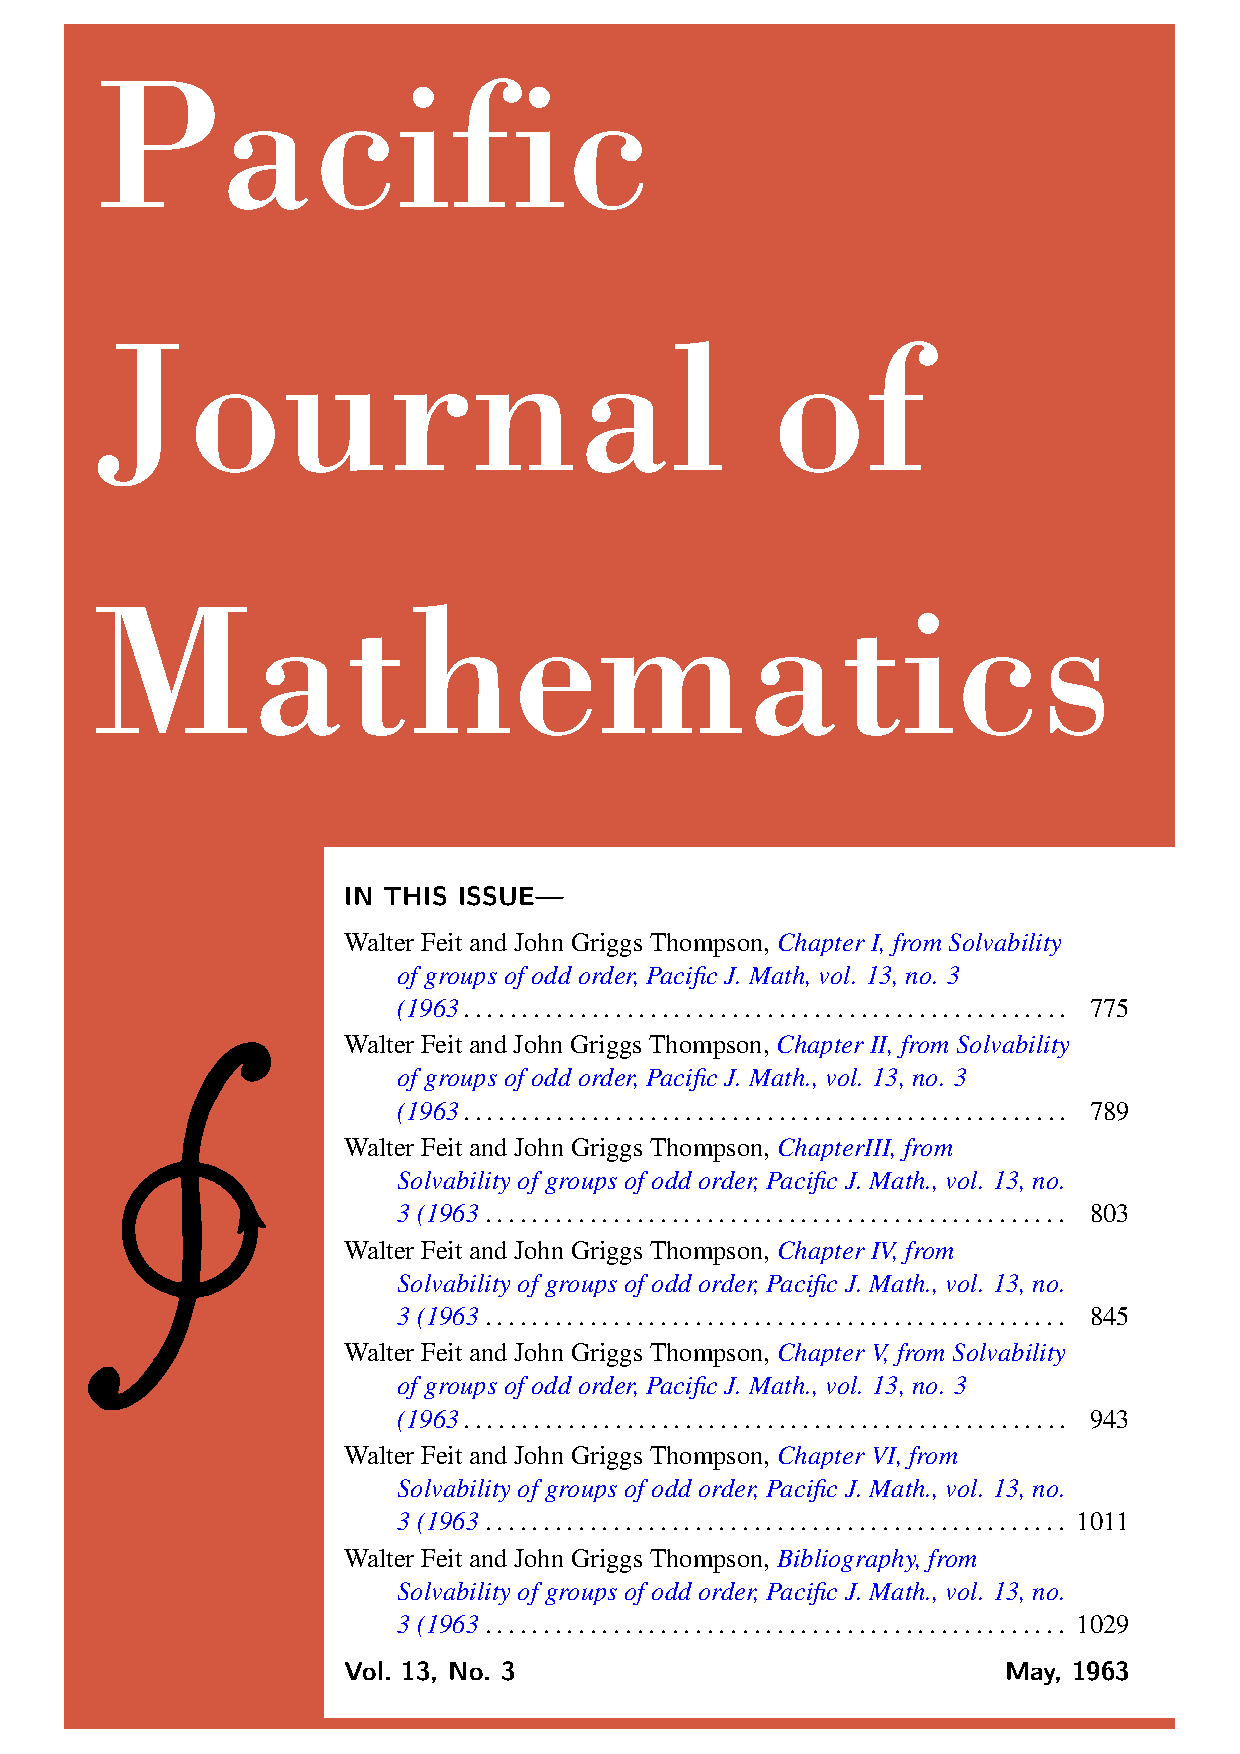
\includegraphics[scale=0.2]{FeitThompson.pdf}
    \caption{The proof of the Feit--Thompson theorem occupies a full volume of 
the Pacific Journal of Mathematics.}
    \label{fig:FeitThompson}
\end{figure}

The Feit--Thompson theorem is one of the starting points
of the classification of finite simple groups (CFSG). 
This classification is one
of the deepest theorems 
of the 20th century. The proof consists of tens of thousands 
of pages in several hundred journal articles written 
by about 100 authors, published mostly between 1955 and 2004.

\begin{theorem}[CFSG]
\index{Classification of simple groups}
\label{thm:CFSG}
Let $G$ be a finite simple group. Then $G$ lies in one (or more) 
of the following families:
\begin{enumerate}
    \item Cyclic groups of prime order.
    \item $\Alt_n$ for $n\geq5$.
    \item Finite groups of Lie type.
    \item 26 sporadic simple groups.
\end{enumerate}
\end{theorem}

Groups of Lie type are finite analogs of simple Lie groups, such as 
$\SL_n(\C)$. A typical example
of a finite simple group of Lie type is
$\PSL_n(p)$ for some prime number $p$, which is defined
as $\SL_n(p)$ over its center. 

The \emph{sporadic simple groups} are 26 groups that do not follow a systematic pattern. 
The first five of the sporadic groups were discovered by Mathieu in the 1860s, and the other 21 
were found between 1965 and 1975.
Several of these groups were predicted to exist before they were constructed, sometimes
just knowing their character tables! 
The full list of sporadic simple groups is as follows:
\begin{itemize}
\item Mathieu groups $M_{11}$, $M_{12}$, $M_{22}$, $M_{23}$ and $M_{24}$.
\item Janko groups $J_1$, $J_2$, $J_3$ and $J_4$.
\item Conway groups $Co_1$, $Co_2$ and $Co_3$.
\item Fischer groups $Fi_{22}$, $Fi_{23}$ and $Fi_{24}$. 
\item Higman–Sims group $HS$.
\item McLaughlin group $McL$.
\item Held group $He$.
\item Rudvalis group $Ru$.
\item Suzuki group $Suz$.
\item O'Nan group $ON$.
\item Harada–Norton group $HN$.
\item Lyons group $Ly$.
\item Thompson group $Th$.
\item Baby Monster group $B$.
\item Monster group $M$.
\end{itemize}

Mathieu groups can be realized 
as automorphism groups of certain very complicated
combinatorial structures known as \emph{Steiner systems}. 
A concrete example: 
\[
M_{11}=\langle (123456789\,10\,11), (37\,11\,8)(4\,10\,56)\rangle,
\]
which is a subgroup of $\Sym_{11}$ of order 7920. The group
$M_{11}$ contains ten irreducible characters, so the
character table of $M_{11}$ is essentially a $10\times 10$ matrix. Let us
use the computer software \lstinline{GAP} 
to see the character table:

\begin{lstlisting}
gap> Display(CharacterTable("M11"));
M11

      2  4  4  1  3  .  1  3  3   .   .
      3  2  1  2  .  .  1  .  .   .   .
      5  1  .  .  .  1  .  .  .   .   .
     11  1  .  .  .  .  .  .  .   1   1

        1a 2a 3a 4a 5a 6a 8a 8b 11a 11b
     2P 1a 1a 3a 2a 5a 3a 4a 4a 11b 11a
     3P 1a 2a 1a 4a 5a 2a 8a 8b 11a 11b
     5P 1a 2a 3a 4a 1a 6a 8b 8a 11a 11b
    11P 1a 2a 3a 4a 5a 6a 8a 8b  1a  1a

X.1      1  1  1  1  1  1  1  1   1   1
X.2     10  2  1  2  . -1  .  .  -1  -1
X.3     10 -2  1  .  .  1  A -A  -1  -1
X.4     10 -2  1  .  .  1 -A  A  -1  -1
X.5     11  3  2 -1  1  . -1 -1   .   .
X.6     16  . -2  .  1  .  .  .   B  /B
X.7     16  . -2  .  1  .  .  .  /B   B
X.8     44  4 -1  . -1  1  .  .   .   .
X.9     45 -3  .  1  .  . -1 -1   1   1
X.10    55 -1  1 -1  . -1  1  1   .   .

A = E(8)+E(8)^3
  = Sqrt(-2) = i2
B = E(11)+E(11)^3+E(11)^4+E(11)^5+E(11)^9
  = (-1+Sqrt(-11))/2 = b11
\end{lstlisting}

Thus the character table of the Mathieu group $M_{11}$ is
given by
\begin{center}
		\begin{tabular}{|c|cccccccccc|}
			\hline
			$\chi_{1}$ & 1 & 1 & 1 & 1 & 1 & 1 & 1 & 1 & 1 & 1\tabularnewline
			$\chi_{2}$ & 10 & 2 & 1 & 2 & 0 & -1 & 0 & 0 & -1 & -1 \tabularnewline
			$\chi_{3}$ & 10 & -2 & 1 & 0 & 0 & 1 & $\alpha$ & $-\alpha$ & -1 & -1\tabularnewline
		    $\chi_{4}$ & 10 & -2 & 1 & 0 & 0 & 1 & $-\alpha$ & $\alpha$ & -1 & -1\tabularnewline
		    $\chi_{5}$ & 11 & 3 & 2 &-1 & 1 & 0 & -1 & -1 & 0 & 0\tabularnewline
			$\chi_{6}$ & 16 & 0 & -2 & 0 & 1 & 0 & 0 & 0 & $\beta$ & $1/\beta$\tabularnewline
			$\chi_{7}$ & 16 & 0 & -2 & 0 & 1 & 0 & 0 & 0 & $1/\beta$ & $\beta$\tabularnewline
			$\chi_{8}$ & 44 & 4 &-1 & 0 &-1 & 1 & 0 & 0 & 0 & 0\tabularnewline
			$\chi_{9}$ & 45 & -3 & 0 & 1 & 0 & 0 &-1 &-1 &  1 & 1\tabularnewline
			$\chi_{10}$ & 55 & -1 & 1 & -1 & 0 & -1 & 1 & 1 & 0 & 0\tabularnewline
			\hline
		\end{tabular}    
\end{center}
where $\alpha=\sqrt{-2}$ and $\beta=\frac{-1-\sqrt{-11}}{2}$. 

The largest sporadic simple group is the \emph{Monster group} $M$ and has order
\[
808017424794512875886459904961710757005754368000000000, 
\]
which is roughly $8\times 10^{53}$. 
The monster group was predicted by Fischer and Griess. 
Griess proved the existence of the Monster group, realizing it as
the automorphism group of a certain space of dimension 196884. 
The group $M$ can be represented as
a subgroup of $\GL_{196883}(\C)$. It has 194 conjugacy classes, so 
the character table is a $194\times 194$ array. 

\begin{problem}
    Formalize the proof of Theorem \ref{thm:CFSG} in a proof assistant. 
\end{problem}

It is precisely due to the vastness of the theorem’s proof, that it is very suitable for formalization. Currently, only mathematicians with an extremely deep understanding of the subject can understand parts of the proof. 
By formalizing the proof in a proof assistant such as \lstinline{Coq} or \lstinline{Lean}, 
the complete proof could be verified at once. 
\lecture{}

\begin{definition}
Let $M$ be a module and $X$ be a subset of $M$. The submodule
of $M$ generated by $X$ is defined as
\[
(X)=\bigcap\{N:N\text{ is a submodule of $M$ that contains $X$}\},
\]
the smallest submodule of $M$ containing $X$. 
\end{definition}

One can prove that  
\[
(X)=\left\{\sum_{i=1}^mr_i\cdot x_i:m\in\Z_{\geq0},\,r_1,\dots,r_m\in R,\,x_1,\dots,x_m\in X\right\}
\]

\begin{definition}
A module $M$ is \textbf{finitely-generated} if $M=(X)$ for some finite subset $X$ of $M$.
\end{definition}

If $X=\{x_1,\dots,x_m\}$ one writes $(X)=(x_1,\dots,x_n)$.
For example, $\Z=(1)=(2,3)$ and $\Z\ne (2)$.

\begin{exercise}
    Let $R$ be the ring of continuous maps $[0,1]\to\R$ with point-wise operations and 
    $M=\prescript{}{R}{R}$. Prove that
    $N=\{f\in R:f(x)\ne0\text{ for finitely many $x$}\}$ is not finitely-generated. 
\end{exercise}

\begin{exercise}
    Let $G=\{g_1,\dots,g_n\}$ be a finite group. Prove that if $M=\C[G]$ is finitely-generated, then
    $M$ is a finite-dimensional complex vector space. 
\end{exercise}

If $f\in\Hom_R(M,N)$ and $M$ is finitely-generated, then 
$f(M)$ is finitely-generated. 

\begin{proposition}
    Let $R$ be a ring and $M$ be a module over $R$. 
    Then $M$ is finitely-generated if and only if $M$ is isomorphic to a quotient of $R^k$ for some $k$.
\end{proposition}

\begin{proof}
    Assume first that $M=(m_1,\dots,m_k)$ is finitely-generated. A routine calculation shows that
    the map
    \[
    \varphi\colon R^k\to M,\quad
    (r_1,\dots,r_k)\mapsto \sum_{j=1}^kr_j\cdot m_j,
    \]
    is a surjective module homomorphism. The first isomorphism theorem implies that 
    $R^k/\ker\varphi\simeq\varphi(R^k)=M$. 
    
    Now assume that there exists a 
    surjective module homomorphism $\varphi\colon R^k\to M$. Since 
    $R^k=(e_1,\dots,e_k)$, where 
    \[
    (e_i)_j=\begin{cases}
    1 & \text{if $i=j$},\\
    0 & \text{if $i\ne j$},
    \end{cases}
    \]
    it follows that $\{\varphi(e_1),\dots,\varphi(e_k)\}$ generates $\varphi(R^k)=M$. Indeed, 
    if $m\in M$, we write $m=\varphi(r_1,\dots,r_k)$ for some $(r_1,\dots,r_k)\in R^k$ 
    and hence 
    \[
    m=\varphi(r_1,\dots,r_k)=\varphi\left(\sum_{i=1}^k r_i\cdot e_i\right)
    =\sum_{i=1}^kr_i\cdot\varphi(e_i).\qedhere
    \]
\end{proof}

\begin{definition}
    Let $R$ be a ring, $M$ be a module over $R$ and $X$ be a subset of $M$. We say that
    $X$ is \textbf{linearly independent} if for each $k\in\Z_{>0}$, $r_1,\dots,r_k\in R$
    and $m_1,\dots,m_k\in X$ such that $\sum_{i=1}^kr_i\cdot m_i=0$, then 
    $r_1=\cdots=r_k=0$. 
\end{definition}

In any ring, the set $\{1\}$ is linearly independent. 

\begin{examples}\
\begin{enumerate}
    \item $\{2,3\}$ is a linear dependent subset of $\Z$.
    \item $\{2\}$ is a linearly dependent subset of $\Z/4$.
    \item Let $R=\Z$, $M=\Q$ and $x\in M\setminus\{0\}$. 
        Then $\{x\}$ is linearly independent subset of $M$. Is $y\in M\setminus\{x\}$, then
        $\{x,y\}$ is linearly dependent.  
\end{enumerate}    
\end{examples}

\begin{examples}
Let $R=M_2(\R)$ and $M=\begin{pmatrix}
        0&\R\\
        0&\R 
    \end{pmatrix}$. Then $\left\{\begin{pmatrix}0&1\\0&0\end{pmatrix}\right\}$ is a minimal generating 
    set and it is linearly independent. 
\end{examples}

\begin{exercise}
    Let $f\in\Hom_R(M,N)$ and $X$ be a subset of $M$. 
    \begin{enumerate}
        \item If $X$ is linearly dependent, then $f(X)$ is linearly dependent.
        \item If $X$ is linearly independent and $f$ is injective, then $f(X)$ is linearly independent. 
        \item If $M=(X)$ and $f$ is surjective, then $N=(f(X))$. 
    \end{enumerate}
\end{exercise}

\begin{definition}
    Let $M$ be a module and $B$ be a subset of $M$. Then $B$ is a \textbf{basis} of $M$ if
    $B$ is linearly independent and $M=(B)$. A module $M$ is said to be \textbf{free} if it admits a basis.   
\end{definition}

As a consequence of Zorn's lemma, 
vector spaces are free. 

\begin{examples}\
\begin{enumerate}
    \item If $R$ is a ring, then $\{1\}$ is a basis of $\prescript{}{R}{R}$, so $\prescript{}{R}{R}$ is free.
    \item If $R$ is a ring, then $R^n$ is free as a module over $R$. 
\end{enumerate}
\end{examples}

\begin{exercise}
    Prove that $\Q$ is not free as a module over $\Z$. 
\end{exercise}

\begin{exercise}
    Let $R$ be a division ring and $M$ be a non-zero and finitely generated module over $R$.
    Prove the following facts:
    \begin{enumerate}
        \item Every finite set of generators contains a basis.
        \item Every linearly independent set can be extended into a basis.
        \item Any two bases contain the same number of elements.
    \end{enumerate}
\end{exercise}

\begin{example}
    $\R[X]$ is a free module (over $\R$) with basis $\{1,X,X^2,\dots\}$. 
\end{example}

\begin{exercise}
    Prove that $\{(a,b),(c,d)\}$ is a basis of $\Z\times\Z$ (as a module over $\Z$) if and only if
    $ad-bc\in\{-1,1\}$. 
\end{exercise}
\chapter{}

\topic{Noetherian modules}

\begin{exercise}
\label{xca:modules_intersection}
    Let $M$ be a module. 
    Prove that the intersection of submodules of $M$ 
    is a submodule of $M$. 
\end{exercise}

\begin{definition}
Let $M$ be a module and $X$ be a subset of $M$. The submodule
of $M$ generated by $X$ is defined as
\[
(X)=\bigcap\{N:N\text{ is a submodule of $M$ that contains $X$}\},
\]
the smallest submodule of $M$ containing $X$. 
\end{definition}

One can prove that  
\[
(X)=\left\{\sum_{i=1}^mr_i\cdot x_i:m\in\Z_{\geq0},\,r_1,\dots,r_m\in R,\,x_1,\dots,x_m\in X\right\}.
\]

\begin{definition}
    \index{Module!finitely generated}
    A module $M$ is \textbf{finitely generated} if $M=(X)$ for some finite subset $X$ of $M$.
\end{definition}

If $X=\{x_1,\dots,x_m\}$ one writes $(X)=(x_1,\dots,x_n)$.
For example, $\Z=(1)=(2,3)$ and $\Z\ne (2)$.

\begin{exercise}
    Let $R$ be the ring of continuous maps $[0,1]\to\R$ with point-wise operations and 
    $M=\prescript{}{R}{R}$. Prove that
    $N=\{f\in R:f(x)\ne0\text{ for finitely many $x$}\}$ is not finitely generated. 
\end{exercise}

\begin{exercise}
    Let $G=\{g_1,\dots,g_n\}$ be a finite group. Prove that if $M=\C[G]$ is finitely generated, then
    $M$ is a finite-dimensional complex vector space. 
\end{exercise}

\begin{example}
    Let $R$ be a ring. The left regular $R$-module $R^3$ is finitely generated 
    by $e_1=(1,0,0)$, $e_2=(0,1,0)$ and $e_3=(0,0,1)$. 
\end{example}

If $f\in\Hom_R(M,N)$ and $M$ is finitely generated, then 
$f(M)$ is finitely generated. To prove this and other similar results, 
we introduce exact sequences (of modules and module homomorphisms). 
A sequence 
	\begin{equation}
	\label{eq:exacta1}	
    \begin{tikzcd}
	0 & M & N & T & 0
	\arrow[from=1-1, to=1-2]
	\arrow["f", from=1-2, to=1-3]
	\arrow["g", from=1-3, to=1-4]
	\arrow[from=1-4, to=1-5]
    \end{tikzcd}
  	\end{equation}
of modules and homomorphism is said to be \textbf{exact} 
if $f$ is injective, $g$ is surjective and $f(M)=\ker g$. For example,
the sequence
\[
\begin{tikzcd}
	0 & M & M\oplus N & N & 0,
	\arrow[from=1-1, to=1-2]
	\arrow["f", from=1-2, to=1-3]
	\arrow["g", from=1-3, to=1-4]
	\arrow[from=1-4, to=1-5]
\end{tikzcd}
\]
where $f(m)=(m,0)$ and $g(m,n)=n$, is exact.

\begin{exercise}
	Let 
\[\begin{tikzcd}
	0 & M & N & T & 0
	\arrow[from=1-1, to=1-2]
	\arrow["f", from=1-2, to=1-3]
	\arrow["g", from=1-3, to=1-4]
	\arrow[from=1-4, to=1-5]
\end{tikzcd}
\]
     be an exact sequence. Prove the following statements: 
     \begin{enumerate}
     \item If $N$ if finitely generated, then $T$ is finitely generated. 
     \item If $M$ and $T$ are finitely generated, then $N$ is finitely generated. 	
     \end{enumerate}
\end{exercise}

\begin{exercise}
\label{xca:submodule_notfg}
Find a finitely generated module that contains a submodule 
that is not finitely generated. 
\end{exercise}

\begin{proposition}
    Let $R$ be a ring and $M$ be a module over $R$. 
    Then $M$ is finitely generated if and only 
    if $M$ is isomorphic to a quotient of $R^k$ for some $k$.
\end{proposition}

\begin{proof}
    Assume first that $M=(m_1,\dots,m_k)$ is finitely generated. A routine calculation shows that
    the map
    \[
    \varphi\colon R^k\to M,\quad
    (r_1,\dots,r_k)\mapsto \sum_{j=1}^kr_j\cdot m_j,
    \]
    is a surjective module homomorphism. The first isomorphism theorem implies that 
    $R^k/\ker\varphi\simeq\varphi(R^k)=M$. 
    
    Now assume that there exists a 
    surjective module homomorphism $\varphi\colon R^k\to M$. Since 
    $R^k=(e_1,\dots,e_k)$, where 
    \[
    (e_i)_j=\begin{cases}
    1 & \text{if $i=j$},\\
    0 & \text{if $i\ne j$},
    \end{cases}
    \]
    it follows that $\{\varphi(e_1),\dots,\varphi(e_k)\}$ generates $\varphi(R^k)=M$. Indeed, 
    if $m\in M$, we write $m=\varphi(r_1,\dots,r_k)$ for some $(r_1,\dots,r_k)\in R^k$ 
    and hence 
    \[
    m=\varphi(r_1,\dots,r_k)=\varphi\left(\sum_{i=1}^k r_i\cdot e_i\right)
    =\sum_{i=1}^kr_i\cdot\varphi(e_i).\qedhere
    \]
\end{proof}

\begin{definition}
    \index{Module!noetherian}
    A module $M$ is \textbf{noetherian} if every sequence $M_1\subseteq M_2\subseteq\cdots$ of submodules of $M$ 
    stabilizes, that is there exists $n$ such that $M_k=M_{n+k}$ for all $k$. 	
\end{definition}

Let $M$ be a module and $X$ be a non-empty 
family of submodules of $M$. We say that $S\in X$ is a \textbf{maximal 
element} (with respect to the inclusion) if $S\subseteq T$ for some $T\in X$ implies $S=T$. 

\begin{proposition}
Let $M$ be a module. The following statements are equivalent:
\begin{enumerate}
\item $M$ is noetherian.
\item All submodules of $M$ are finitely generated.
\item Every non-empty family of submodules of $M$ has a maximal element. 	
\end{enumerate}
\end{proposition}

\begin{proof}
	We first prove $2)\implies1)$. If $S_1\subseteq S_2\subseteq\cdots$ is an increasing 
        sequence of submodules of $M$, 
	it follows that $S=\cup_{i\geq 1}S_i$ is a submodule\footnote{In general, the union of submodules is not a submodule. Here $\cup_jS_j$ is a submodule because we have an increasing sequence $S_1\subseteq S_2\subseteq\cdots$ of submodules.} 
 of $M$. Since $S$ is finitely generated, 
	$S=(x_1,\dots,x_n)$ for some $x_1,\dots,x_n\in M$. It follows that 
	$x_1,\dots,x_n\in S_N$ for some positive integer $N$. Thus 
	$S\subseteq S_N$ and hence $S_N=S_{N+k}$ for all $k$. 
	
	We now prove $1)\implies3)$. Let $F$ be a non-empty family of submodules of $M$ with no maximal elements. 
	Let $S_1\in F$. Since $S_1$ is not maximal in $F$, there exists $S_2\in F$ such that $S_1\subsetneq S_2$. 
	Having constructed with this method the submodules $S_1\subsetneq\dots\subsetneq S_k$, since $S_k$ is not
	maximal in $F$, there exists $S_{k+1}\in F$ such that $S_k\subsetneq S_{k+1}$. 
	This means that the sequence 
	$S_1\subsetneq S_2\subsetneq\cdots$ does not stabilize. 
	
	We finally prove $3)\implies2)$. Let $S$ be a submodule of $M$ and let 
	\[
	F=\{T\subseteq S:T\text{ finitely generated submodule of $M$}\}.
	\]
	Note that $F\ne\emptyset$, as $\{0\}\in F$. 
	Then $F$ has a maximal element $N$. Thus
	$N$ is a finitely generated submodule of $M$ such that $N\subseteq S$. We may assume that 
	$N=(n_1,\dots,n_k)$. If $N=S$, then, in particular, $S$ is finitely generated. Suppose that
	$N\ne S$ and let $x\in S\setminus N$. It follows that  
	$N\subseteq (n_1,\dots,n_k,x)\subseteq S$. Since 
	$(n_1,\dots,n_k,x)\in F$ and $N$ is maximal, it follows that 
	$N=(n_1,\dots,n_k,x)$, a contradiction
	to $x\not\in N$. 
\end{proof}

The previous theorem shows that every noetherian module is finitely generated. 

\begin{exercise}
\label{xca:Pruffer}
Find a non-noetherian module such that every proper submodule is finitely generated. 	
\end{exercise}

\begin{exercise}
\label{xca:exacta_noetheriano}
	Let   
\[\begin{tikzcd}
	0 & M & N & T & 0
	\arrow[from=1-1, to=1-2]
	\arrow["f", from=1-2, to=1-3]
	\arrow["g", from=1-3, to=1-4]
	\arrow[from=1-4, to=1-5]
\end{tikzcd}
\]
     be an exact sequence. Prove the following statements:
     \begin{enumerate}
     	\item If $N$ is noetherian, then $M$ and $T$ are noetherian.
     	\item If $M$ and $T$ are noetherian, then $N$ is noetherian.
     \end{enumerate}	
\end{exercise}

\begin{exercise}
\label{xca:regular_noetheriano}
A commutative ring $R$ is noetherian if and only if $\prescript{}{R}R$ is noetherian.	
\end{exercise}

\begin{exercise}
\label{xca:directa_noetheriano}
If $M_1,\dots,M_n$ are noetherian, then $M_1\oplus\cdots\oplus M_n$ is noetherian. 	
\end{exercise}

The previous exercise cannot be extended to infinitely many modules. Why?
%For example, $\Z^{\Z}$ is not noetherian, as it is not finitely generated. 

\begin{proposition}
If $R$ is noetherian and $M$ is a finitely generated module, then $M$ is noetherian. 
\end{proposition}

\begin{proof}
    Assume that $M=(m_1,\dots,m_k)$. There exists a surjective homomorphism  
$R^k\to M$, $(r_1,\dots,r_k)\mapsto \sum_{i=1}^k r_i\cdot m_i$, where
$R^k=\oplus_{i=1}^k R$. Since $R$ is noetherian, $R^k$ is noetherian. Thus $M$ is noetherian.	
\end{proof}

\topic{Quotient fields}

Let $R$ be an integral domain and $S=R\setminus\{0\}$. 
On $R\times S$ we define the following relation:
\[
(r,s)\sim (r_1,s_1)\Longleftrightarrow rs_1-r_1s=0.
\]

\begin{exercise}
Prove that $\sim$ is an equivalence relation.
\end{exercise}

The equivalence class of $(r,s)$ will be denoted by $r/s$ or $\frac{r}{s}$. 

It is possible to prove that the set 
$K(R)=(R\times S)/{\sim}$ of equivalence classes is a field 
with the operations 
\begin{equation}
\label{eq:K(R)}
\frac{r}{s}+\frac{r_1}{s_1}=\frac{rs_1+r_1s}{ss_1},
\quad
\frac{r}{s}\frac{r_1}{s_1}=\frac{rr_1}{ss_1}.
\end{equation}

\begin{definition}
$K(R)$ is known as the \textbf{quotient field} of $R$. 
\end{definition}

Simple example: $K(\Z)=\Q$.

\begin{exercise}
Let $R$ be an integral domain. 
Prove that $K(R)$ is a field. 
\end{exercise}

To prove that $K(R)$ is a field, one first needs to prove that 
the operations~\eqref{eq:K(R)} are well-defined. For example, let us check the addition is well-defined. 
If $r/s\sim r'/s'$ and $r_1/s_1\sim r_1'/s_1'$, then
$r/s+r_1/s_1\sim r'/s'+r_1'/s_1'$. In fact, 
since $r/s\sim r'/s'$, it follows that $rs'-r's=0$. Similarly, $r_1s_1'-r_1's_1=0$, as $r_1/s_1\sim r_1'/s_1'$. Thus 
\begin{gather*}
\frac{rs_1+r_1s}{ss_1}=\frac{r's_1'+r_1's'}{s's_1'}
\shortintertext{as}
(rs_1+r_1s)s's_1'=rs_1s's_1'+r_1ss's_1'
=r'ss_1s_1'+r_1's_1ss'
=(r's_1'+r_1's)ss_1.
\end{gather*}


\topic{Free modules}

\begin{definition}
    Let $R$ be a ring, $M$ be a module over $R$ and $X$ be a subset of $M$. We say that
    $X$ is \textbf{linearly independent} if for each $k\in\Z_{>0}$, $r_1,\dots,r_k\in R$
    and $m_1,\dots,m_k\in X$ such that $\sum_{i=1}^kr_i\cdot m_i=0$, then 
    $r_1=\cdots=r_k=0$.  
\end{definition}

In any ring, the set $\{1\}$ is linearly independent. 

A set is said to be 
\textbf{linearly dependent} if it is not linearly independent.
    
\begin{examples}\
\begin{enumerate}
    \item $\{2,3\}$ is a linearly dependent subset of $\Z$.
    \item $\{2\}$ is a linearly dependent subset of $\Z/4$.
    \item Let $R=\Z$, $M=\Q$ and $x\in M\setminus\{0\}$. 
        Then $\{x\}$ is a linearly independent subset of $M$. Is $y\in M\setminus\{x\}$, then
        $\{x,y\}$ is linearly dependent.  
\end{enumerate}    
\end{examples}

A generating set $X$ for a module $M$ is \emph{minimal} if 
$X\setminus\{x\}$ is no longer a generating set of $M$ for all $x\in X$. 
In vector spaces, a subset of the vector space is a basis
if and only if it is a minimal generating set. This is no longer true 
for arbitrary modules.

\begin{examples}
Let $R=M_2(\R)$ and $M=\begin{pmatrix}
        0&\R\\
        0&\R 
    \end{pmatrix}$. Then $\left\{\begin{pmatrix}0&1\\0&0\end{pmatrix}\right\}$ is a minimal generating 
    set and it is not linearly independent. 
\end{examples}

However, one can prove that each module's basis is a minimal generating set. 
% roman 4.4, page 116

\begin{exercise}
\label{xca:LI}
    Let $f\in\Hom_R(M,N)$ and $X$ be a subset of $M$. 
    \begin{enumerate}
        \item If $X$ is linearly dependent, then $f(X)$ is linearly dependent.
        \item If $X$ is linearly independent and $f$ is injective, then $f(X)$ is linearly independent. 
        \item If $M=(X)$ and $f$ is surjective, then $N=(f(X))$. 
    \end{enumerate}
\end{exercise}

\begin{definition}
    Let $M$ be a module and $B$ be a subset of $M$. Then $B$ is a \textbf{basis} of $M$ if
    $B$ is linearly independent and $M=(B)$. A module $M$ is said to be \textbf{free} if it admits a basis.   
\end{definition}

As a consequence of Zorn's lemma, 
vector spaces are free. 

\begin{examples}\
\begin{enumerate}
    \item If $R$ is a ring, then $\{1\}$ is a basis of $\prescript{}{R}{R}$, so $\prescript{}{R}{R}$ is free.
    \item If $R$ is a ring, then $R^n$ is free as a module over $R$. 
\end{enumerate}
\end{examples}

\begin{exercise}
    Prove that $\Z/4$ is free as a $\Z/4$ module and that the submodule 
    $\{0,2\}\subseteq \Z/4$ is not free as a $\Z/4$-module.
\end{exercise}
\begin{exercise}
    Prove that $\Q$ is not free as a module over $\Z$. 
\end{exercise}

\begin{exercise}
\index{Module!over a division ring}
\label{xca:linear_algebra}
    Let $R$ be a division ring and $M$ be a non-zero and finitely generated module over $R$.
    Prove the following facts:
    \begin{enumerate}
        \item Every finite set of generators contains a basis.
        \item Every linearly independent set can be extended into a basis.
        \item Any two bases contain the same number of elements.
    \end{enumerate}
\end{exercise}

The previous exercise states that modules over division rings 
are like vector spaces over fields. In particular, 
such modules have dimensions.

\begin{example}
    $\R[X]$ is a free module (over $\R$) with basis $\{1,X,X^2,\dots\}$. 
\end{example}

\begin{exercise}
    Prove that $\{(a,b),(c,d)\}$ is a basis of $\Z\times\Z$ 
    (as a module over $\Z$) if and only if
    $ad-bc\in\{-1,1\}$. 
\end{exercise}

\begin{example}
If $u\in\mathcal{U}(R)$, then $\{u\}$ is a basis of $\prescript{}{R}R$. Conversely, if $R$ is an integral domain and 
$\{z\}$ is a basis of $\prescript{}{R}R$, then $z\in\mathcal{U}(R)$. Since 
$1=yz$ for some $y\in R$, it follows that $zy=1$, as  
\[
(zy-1)z=z(yz)-z=z1-z=z-z=0.
\]	
\end{example}

If $R$ is a ring and $I$ is a set, 
\[
R^{(I)}=\{f\colon I\to R:f(x)=0\text{ for all but finitely many $x\in I$}\}
\]
is a module (over $R$) with 
$(f+g)(x)=f(x)+g(x)$ and $(rf)(x)=rf(x)$ for all $f,g\in R^{(I)}$, $x\in I$ and $r\in R$. 
Note that 
every element 
of $R^{(I)}$ can be written uniquely as
a finite sum of the form 
\[
\sum_{i\in I}r_i\delta_i,
\]
where the $r_i$ are elements of $R$ and only finitely many of them are non-zero, and 
\[
\delta_i(j)=\begin{cases}
1 & \text{if $i=j$},\\
0 & \text{otherwise}.
\end{cases}.
\]
One proves
that
\[
R^{(I)}\simeq\bigoplus_{i\in I}R.
\]

\begin{example}
If $I$ is a non-empty set, the module $R^{(I)}$ is free with basis 
$\{\delta_i:i\in I\}$, where 
\[
\delta_i(j)=\begin{cases}
	1 & \text{if $i=j$},\\
	0 & \text{if $i\ne j$.}
	\end{cases}	
\]
\end{example}

\begin{example}
If $R=M_2(\Z)$, then $M=\prescript{}{R}R$ is free with basis $\left\{\begin{pmatrix}
    1&0\\0&1\end{pmatrix}\right\}$. The submodule 
$N=\begin{pmatrix}\Z&0\\\Z&0\end{pmatrix}$ does not admits a basis as a module over $R$.
\end{example}

In modules, the size of a basis is not an invariant of the module.  

\begin{example}
Let $V$ be the complex vector space with infinite basis $e_0,e_1,e_2,\dots$ and let 
$R=\End(V)$ with the ring structure given by 
\[
(f+g)(v)=f(v)+g(v),\quad
(fg)(v)=f(g(v))
\]
for $f,g\in R$ and $v\in V$. 

Let $M=\prescript{}{R}R$. 
The set $\{\id\}$ is a basis for $R$.  
We claim that $M$ admits a basis with two elements. If
$r,s\in R$ are such that 
\begin{align*}
&r(e_{2n})=e_n, && r(e_{2n+1})=0,\\
&s(e_{2n})=0,&& s(e_{2n+1})=e_{2n},
\end{align*}
then $\{r,s\}$ is a basis of $M$. 
If $f\in R$, then
$f=\alpha r+\beta s$, where $\alpha\colon V\to V$, $e_n\mapsto f(e_{2n})$ for all $n$, and
$\beta\in V\to V$, $e_n\mapsto f(e_{2n+1})$ for all $n$. In fact,
\begin{align*}
&(\alpha r+\beta s)(e_{2n})=\alpha(r(e_{2n}))+\beta(s(e_{2n}))=f(e_{2n}),\\
&(\alpha r+\beta s)(e_{2n+1})=\alpha(r(e_{2n+1}))+\beta(s(e_{2n+1}))=f(e_{2n+1}).
\end{align*}
Moreover, $\{r,s\}$ is linearly independent. Indeed, if $\alpha r+\beta s=0$ for some $\alpha,\beta\in R$,  
Evaluation on $e_{2n}$ yields $\alpha=0$ and evaluation on $e_{2n+1}$ yields $\beta=0$.   
\end{example} 

\begin{example}
If $M$ is a free module with basis $X$ and $N$ 
is a free module with basis $Y$, then 
$M\oplus N$ is a free module with basis 
\[
\{(x,0):x\in X\}\cup \{(0,y):y\in Y\}.
\]	
\end{example}

\begin{exercise}
Let $R$ be a commutative ring. If $M$ and $N$ 
are free and finitely generated, then 
$\Hom_R(M,N)$
is free and finitely generated.
\end{exercise}

% Como $R$ es conmutativo, $\Hom_R(M,N)$ es un $R$-módulo. Si $\{m_1,\dots,m_k\}$ es base de $M$ 
% y $\{n_1,\dots,n_l\}$ es base de $N$, entonces definimos para cada $i\in\{1,\dots,k\}$ y $j\in\{1,\dots,l\}$ 
% definimos $f_{ij}$ 
% \[
% f_{ij}(m_k)=\begin{cases}
% n_j & \text{si $k=i$},\\
% 0 & \text{si $k\ne i$}.
% \end{cases}
% \]
% Entonces $\{i_ij}$ es base de $\Hom_R(M,N)$. 
Some properties of free modules:

\begin{proposition}
If $M$ is free, then there exists a subset $\{m_i:i\in I\}$ of $M$ 
such that for each $m\in M$ there exist unique $r_i\in R$, $i\in I$, 
where $r_i=0$ except for finitely many $i\in I$ 
such that $m=\sum r_i\cdot m_i$. 
\end{proposition}

\begin{proof}
Since $M$ is free, there exists a basis $\{m_i:i\in I\}$ of $M$. If $m\in M$,
$m=\sum r_i\cdot m_i$ (finite sum) for some $r_i\in I$. We claim that
the $r_i$'s are unique. If $m=\sum s_i\cdot m_i$, then
$\sum (r_i-s_i)\cdot m_i=0$. Since $\{m_i:i\in I\}$ 
is linearly independent, $r_i=s_i$ for all $i\in I$.  	
\end{proof}

\begin{proposition}
\label{pro:libre}
Let $M$ be a free module over $R$ with basis $\{m_i:i\in I\}$ and let $N$ be a module over $R$. 
If $\{n_i:i\in I\}\subseteq N$, then 
there exists a unique $f\in\Hom_R(M,N)$ such that
$f(m_i)=n_i$ for all $i\in I$.  
\end{proposition}

\begin{proof}[Sketch of the proof]
Note that the unique homomorphism $f\colon M\to N$ is defined as 
$f(\sum r_i\cdot m_i)=\sum r_i\cdot n_i$.  	
\end{proof}

Another application:

\begin{example}
There is no surjective homomorphism $\Z\to\Z\times\Z$ (of modules over $\Z$). 
If $f\colon\Z\to\Z\times\Z$ is a surjective homomorphism, 
let $\{u,v\}$ a basis of $\Z\times\Z$. Then $f(k)=u$ and $f(l)=v$ for some $k,l\in\Z$. Proposition~\ref{pro:libre} implies 
that there exists a homomorphism $g\colon\Z\times\Z\to\Z$ such that $g(u)=k$ and $g(v)=l$. 
In particular, $f g=\id_{\Z\times\Z}$ and hence 
$g$ is injective. Since  
\[
g(lu-kv)=lg(u)-kg(v)=lk-kl=0,
\]
it follows that $lu-kv=0$ and thus $k=l=0$, as $\{u,v\}$ is linearly independent, a contradiction
\end{example}

Another important property:

\begin{proposition}
If $M$ is a free $R$-module, then $M\simeq R^{(I)}$ for some set $I$.
\end{proposition}

\begin{proof}
Suppose that $M$ has basis $\{m_i:i\in I\}$. There exists a unique homomorphism
$f\in\Hom_R(M,R^{(I)})$ such that  
$f(m_i)=\delta_i$ for all $i\in I$, where 
\[
\delta_i(j)=\begin{cases}
	1 & \text{si $i=j$},\\
	0 & \text{si $i\ne j$.}
	\end{cases}	
\]	
We claim that $f$ is an isomorphism. We first prove that the map $f$ is surjective: if $(r_i)_{i\in I}\in R^{(I)}$, then
$f(\sum r_i\cdot m_i)=(r_i)_{i\in I}$. Let us prove that $f$ is injective: 
\[
0=f(\sum r_i\cdot m_i)=\sum r_i\cdot f(m_i)=\sum r_i\cdot\delta_i\implies r_i=0\text{ for all $i\in I$}.\qedhere
\]
\end{proof}

\begin{corollary}
Every module is (isomorphic to) a quotient of a free module.
\end{corollary}

\begin{proof}
Let $M$ be a module. We claim that there exists a free module $L$ and a surjective homomorphism $f\in\Hom_R(L,M)$. Then
$L/\ker f\simeq M$. Let $\{m_i:i\in I\}$
be a generating set of $M$ (note that such a generating set always exists, as one could take, for example, the set
$\{m:m\in M\}$) and let $L=R^{(I)}$. Then $L$ is free and $f\colon R^{(I)}\to M$, $\delta_i\mapsto m_i$, is a surjective 
homomorphism.
\end{proof}

Another important property of free modules: free modules are
\emph{projective}. 

\begin{proposition}
	\label{pro:free=>projective}
	If $M$ is a free module and $f\in\Hom_R(N,T)$ is surjective and
	$h\in\Hom_R(M,T)$, then there exists $\varphi\in\Hom_R(M,N)$ such that
	$f\varphi=h$. 
\end{proposition}

\begin{proof}
    We will prove that 
    there exists a homomorphism $\varphi$ that makes
    the diagram
    \[\begin{tikzcd}
	& M \\
	N & T & 0
	\arrow["f"', from=2-1, to=2-2]
	\arrow[from=2-2, to=2-3]
	\arrow["h", from=1-2, to=2-2]
	\arrow["\varphi"', dashed, from=1-2, to=2-1]
\end{tikzcd}\]
    commutative. 
	Let $\{m_i:i\in I\}$ be a basis of $M$. Since $f$ is surjective, for each
	$i\in I$ there exists $n_i\in N$ such that $f(n_i)=h(m_i)$. Since  $M$ is
	free, there exists a unique homomorphism $\varphi\colon M\to N$ such that
	$\varphi(m_i)=n_i$ for all $i\in I$. Thus homomorphism is such that
	$f\varphi=h$. 
\end{proof}

A consequence of the previous proposition
that we will use later:

\begin{proposition}
\label{pro:split}
	Let 
	\[
	   \begin{tikzcd}
        0 & A & B & C & 0
        \arrow[from=1-1, to=1-2]
        \arrow["f", from=1-2, to=1-3]
        \arrow["g", from=1-3, to=1-4]
        \arrow[from=1-4, to=1-5]
    \end{tikzcd}
	\]
	be an exact sequence of modules.  If $C$ is free, then $A\oplus C\simeq B$. 
\end{proposition}

\begin{proof}
    By considering the diagram
\[\begin{tikzcd}
	& C \\
	B & C & 0
	\arrow["g"', from=2-1, to=2-2]
	\arrow[from=2-2, to=2-3]
	\arrow[equal, no head, from=1-2, to=2-2]
	\arrow["h"', dashed, from=1-2, to=2-1]
\end{tikzcd}\]
	the previous proposition 
	yields a homomorphism $h\colon C\to B$
	such that $gh=\id_C$. In fact, let $\{c_i:i\in I\}$ be a basis of $C$.
	For each $i\in I$ let $b_i\in B$ be such that $g(b_i)=c_i$. The map 
	$h\colon C\to B$, $h(\sum r_i\cdot c_i)=\sum r_i\cdot b_i$, is a module homomorphism 
	such that $gh=\id_C$. 

	Let $\varphi\colon A\oplus C\to B$, $(a,c)\mapsto f(a)+h(c)$. A simple
	calculation shows that $\varphi$ is a module homomorphism. 

	We prove that $\varphi$ is 
	injective. If $\varphi(a,c)=0$, then $f(a)+h(c)=0$. By applying $g$ we get that
	$0=g(f(a))+g(h(c))=c$ and hence, since $f$ is injective and
	$f(a)=0$, is follows that $(a,c)=(0,0)$. 
		
	Now we prove that $\varphi$ is surjective. 
	Let $b\in B$. 
	We need to find $(a,c)\in A\oplus C$ such that $\varphi(a,c)=b$. 
	Let $c=g(b)\in C$. Since
	\[
		g(b-h(c))=g(b)-gh(c)=g(b)-c,
	\]
	it follows that $b-h(c)\in \ker g=f(A)$. This means
	that $b-h(c)=f(a)$ for some $a\in A$. Now $b\in \varphi(A\oplus C)$, as
	\[
		\varphi(a,c)=f(a)+h(c)=b-h(c)+h(c)=b.\qedhere
	\]
\end{proof}

What can we say about the number of elements of a basis? 
If $M$ has a finite basis, then every basis of $M$ will be finite. To prove
this, let $M$ be a module 
and $E=\{e_i:i\in I\}$ be a basis of $M$. If $M$ is finitely generated, say 
$M=(m_1,\dots,m_k)$, write each $m_j$ as a (finite) linear combination of elements
of $E$. Then there exists 
a finite set $\{e_1,\dots,e_m\}$ that generates $M$. Since 
$E$ is a basis, it follows that
$\{e_1,\dots,e_m\}=E$ and hence $E$ is finite.  

\begin{exercise}
\label{xca:cardinality}
    Let $M$ be a free module with an infinite basis $E$. Prove
    that every basis of $M$ has cardinality $|E|$. 
\end{exercise}

Under additional assumptions the previous exercise also holds for 
finite bases. 

\begin{theorem}
Let $R$ be an integral domain. If $M$ is free with a finite basis, then 
any two bases of $M$ have the same number of elements.
\end{theorem}

\begin{proof}
Let $K=K(R)$ be the field of fractions of $R$. Note that 
$V=\Hom_R(M,K)$ is an abelian group and hence it 
is a vector space (over $K$) with 
\[
(\lambda f)(m)=\lambda f(m),
\]
where $\lambda\in K$, $f\in V$ and $m\in M$.

The vector space $V$ has a well-defined dimension. 
Let us compute $\dim V$. Let $\{e_1,\dots,e_n\}$ be a basis of $M$. 
For each $i\in\{1,\dots,n\}$ let 
\[
f_i\colon M\to K,\quad
e_j\mapsto\begin{cases}
1 & \text{si $i=j$},\\
0 & \text{si $i\ne j$}.
\end{cases}
\]
We claim that $\{f_1,\dots,f_n\}$ is basis of  $V$. It generates $V$, as  
if $f\in V$, then 
\[
f=\sum_{i=1}^n f(e_i)f_i,
\]
as these homomorphisms coincide in the elements of a basis of $M$, that is 
$f(e_j)=(\sum_{i=1}^n f(e_i)f_i)(e_j)$ for all $j\in\{1,\dots,n\}$.    
Moreover, $\{f_1,\dots,f_n\}$ is linearly independent, as if $0=\sum_{i=1}^n\lambda_if_i$, 
then, evaluating on each $e_j$, it follows that 
\begin{align*}
0=\left(\sum_{i=1}^n \lambda_if_i\right)(e_j)=\lambda_j
\end{align*}
for all $j\in\{1,\dots,n\}$. Thus $n=\dim V$. 
\end{proof}

The previous result can be proved for commutative rings. 

\begin{definition}
Let $R$ be an integral domain. If $M$ is a free 
finitely generated module, we define
the \textbf{rank} of $M$ as the size of a basis of $M$. If $M$ is not finitely generated, 
we say that the rank of $M$ is infinite. 
\end{definition}

The rank of a module $M$ will be denoted by $\rank(M)$.   

\section{}


\subsection{Modules over principal domains}

Recall that a principal domain is a commutative ring where 
every ideal is principal, i.e. generated by one element and 
such that $xy=0$ implies $x=0$ or $y=0$. 

\begin{theorem}
\label{thm:rango}
Let $R$ be a principal domain. If $F$ is a finitely generated free $R$-module and 
$N$ is a submodule of $F$, then $N$ is free and 
$\rank(N)\leq\rank(F)$. In particular, $N$ is finitely generated. 
\end{theorem}

\begin{proof}
	We proceed by induction on $n=\rank(F)$. Si $n=1$, then
	$F\simeq\prescript{}{R}R$ 
	and since $R$ is commutative the submodules of $F$ are exactly the ideals of $R$. In particular,
	$N=(r)$ for some $r\in R$. If $r=0$, then $N=\{0\}$ and the result holds. If $r\ne 0$, then 
	$\{r\}$ is basis of $N$ (since $R$ is a domain) and the result holds.
	
	Assume now that the result holds for all free modules of rank $<n$. Let $F$ be a free module of
	rank $n$ and 
	$\{f_1,\dots,f_n\}$ be basis of $F$. Let $F_n=(f_1,\dots,f_{n-1})$. By the inductive hypothesis, 
	$U=N\cap F_n$ is free of rank $\leq n-1$. Let 
	$\{n_1,\dots,n_k\}$ be a basis of $U$ (by convention, if $U=\{0\}$, then $k=0$). If 
	$f\in F$, there exist unique $r_1,\dots,r_n\in R$ such that  
	\[
	f=\sum_{i=1}^n r_i\cdot f_i.
	\]
	There exists a well-defined surjective homomorphism 
	\[
	\varphi\colon F\to R,
	\quad
	\sum_{i=1}^nr_i\cdot f_i\mapsto r_n.
	\] 
	If $\varphi(N)=\{0\}$, then $N\subseteq (f_1,\dots,f_{n-1})$ and thus $N=U$. 
	If $\varphi(N)\ne\{0\}$, then $\varphi(N)$ is an ideal of 
	$R$, say $\varphi(N)=(x)$ for some $x\in R\setminus\{0\}$. Let $n_{k+1}\in N$ 
	be such that $\varphi(n_{k+1})=x$. 
    We claim that $\{n_1,\dots,n_k,n_{k+1}\}$ is basis of $N$. We first proves that 
    this is a generating set. 
	If $n\in N$, then $\varphi(n)=rx$ 
	for some $r\in R$. Thus $n-r\cdot n_{k+1}\in N\cap\ker\varphi=N\cap F_n=U$, as  
	$\varphi(n-r\cdot n_{k+1})=0$. In particular, 
	\[
	n-r\cdot n_{k+1}\in (n_1,\dots,n_k)\implies  
	n\in (n_1,\dots,n_k,n_{k+1}).
	\]
	We claim that 
	$\{n_1,\dots,n_k,n_{k+1}\}$ is linearly independent. If 
	\[
	0=\sum_{i=1}^{k+1}r_i\cdot n_i,
	\]
	for some $r_1,\dots,r_{k+1}\in R$, then, since 
	$\varphi(n_i)=0$ for all $i\in\{1,\dots,k\}$,
	\[
	0=\varphi(r_{k+1}\cdot n_{k+1})=r_{k+1}x.
	\]
	This implies that $r_{k+1}=0$. Thus $\sum_{i=1}^kr_i\cdot n_i=0$. Since
	$\{n_1,\dots,n_k\}$ is basis of $U$, we conclude that 
	$r_1=\dots=r_k=0$. 
\end{proof}

The previous theorem also holds for infinite bases. However, 
the proof requires the use of Zorn's lemma. 
% reference?
	
% \begin{corollary}
% Sea $R$ un dominio de ideales principales. Si $M$ es proyectivo y finitamente generado, 
% entonces $M$ es libre.
% \end{corollary}

% \begin{proof}
% Supongamos que $M=(m_1,\dots,m_k)$. Sabemos que $M$ es sumando directo de un libre $F$. Fijemos una base de $F$ y sea 
% $X=\{f_1,f_2,\dots\}$ un subconjunto finito de esa base de $F$ tal que
% \[
% m_j=\sum_{i=1}^{n_j}r_{ij}\cdot f_i
% \]
% para ciertos $r_{ij}\in R$ y ciertos $n_1\dots,n_k\in\N$. 
% Por construcción, $X$ es linealmente indepdendiente y $M=(X)$. 
% \end{proof}

% El corolario anterior vale también para módulos arbitrarios. La demostración puede
% consultarse por ejemplo en~\cite[I, Theorem 5.1]{MR1438546}.

\begin{corollary}
Let $R$ be a principal domain. If $M$ is a finitely generated $R$-module and $N$ 
is a submodule of $M$, then $N$ is finitely generated.   
\end{corollary}

\begin{proof}
There exists a free module $F$ of finite rank and a surjective homomorphism
$\varphi\colon F\to M$. Since $N_1=\varphi^{-1}(N)$ is a submodule of $F$, 
the previous theorem implies that  
$\rank(N_1)\leq\rank F<\infty$. If $\{x_1,\dots,x_k\}$ is basis of $N_1$, then
$\{\varphi(x_1),\dots,\varphi(x_k)\}$ is a generating set of 
$\varphi(N_1)=\varphi(\varphi^{-1}(N))=N$, as 
$\varphi$ is surjective. $N$ is generated by 
$\leq k=\rank(N_1)\leq\rank(F)<\infty$ elements.  
\end{proof}

Some exercises:

\begin{exercise}
\label{xca:rank}
    Let $R$ be a principal domain and 
    let $M$ be a free $R$-module. If $S$ is a submodule of $M$ such that
    $M/S$ is free, then $M\simeq S\oplus (M/S)$. Moreover,  
	$S$ is free and 
	\[
	\rank(M)=\rank(S)+\rank(M/S).
	\] 
\end{exercise}

\begin{exercise}
\label{xca:n_elements}
    Let $R$ be a principal domain. 
    If $M$ is a free $R$-module of rank $n$, then
    every linearly independent subset of $M$ 
    contains at most $n$ elements. 
\end{exercise}

\begin{exercise}
    Let $R$ be a principal domain. 
    and $M$ and $N$ be free $R$-modules. Prove that 
    $M\simeq N$ if and only if $\rank(M)=\rank(N)$. 	
\end{exercise}

\begin{exercise}
\label{xca:base}
    Let $R$ be a principal domain. 
    If $M$ is a free $R$-module of finite rank $n$ and $\{s_1,\dots,s_n\}$ 
    is a generating set, then $\{s_1,\dots,s_n\}$ is a basis of $M$.
\end{exercise}

\index{Annihilator!of a module}
\index{Annihilator!of an element}
If $M$ is an $R$-module, the \emph{annihilator} of $M$ 
is defined as 
\[
\Ann(M)=\{r\in R:r\cdot m=0\text{ for all $m\in M$}\}.
\] 
For $m\in M$ let 
\[
\Ann(m)=\{r\in R:r\cdot m=0\}.
\]  
Note that $\Ann(M)=\cap_{m\in M}\Ann(m)$. 
It is an exercise to show that both 
$\Ann(M)$ and $\Ann(m)$ are ideals of $R$. 
If $r\in R$, the annihilator of $r$ in $M$ 
is defined as 
\[
\Ann_M(r)=\{m\in M:r\cdot m=0\}.
\] 
It is an exercise to show that $\Ann_M(r)$ is a submodule of 
$M$. 

\begin{exercise}
Let $M$ be an $R$-module and $m\in M$ be such that $\Ann(m)=(r)$ 
for some $r\in R$. 
Let $p\in R$ be an irreducible element. Prove the following statements: 
\begin{enumerate}
\item If $p$ divides $r$, then $(m)/(p\cdot (m))\simeq R/(p)$.
\item If $p$ does not divide $r$, then $p\cdot (m)=(m)$.
\end{enumerate}
\end{exercise}

% Demostremos la primera afirmación. Sea $\varphi\colon R\to (m)$, $s\mapsto s\cdot m$, y 
% sea $f=\pi\circ \varphi\colon R\to (m)/p\cdot (m)$, donde $\pi\colon (m)\to (m)/p\cdot (m)$ es 
% el epimorfismo canónico. Veamos que $\ker f=(p)$. Trivialmente vale 
% que $\ker f\supseteq (p)$. Por otro lado, si $s\in R$ es tal que
% s\cdot m\in p\cdot (m)$, entonces, como $r=pt$ para algún $t\in R$, $s\cdot m=t\cdot (p\cdot m)$.
% Como $f$ es epimorfismo por ser composición
% de epimorfismos, se tiene que $R/(p)\simeq (m)/p\cdot (m)$.  

% Demostremos ahora la segunda afirmación. Como $p$ y $r$ son coprimos, existen 
% $a,b\in R$ tales que $ap+br=1$. Como $r\cdot \m=0$ pues $\Ann(m)=(r)$, 
% $m=1\cdot m=(ap+br)\cdot m=p\cdot (a\cdot m)\in p\cdot (m)$.  

\index{Torsion!of a module}
\index{Torsion-free module}
\index{Torsion!module}
The \emph{torsion} of an $R$-module $M$ 
is defined as the subset 
\[
T(M)=\{m\in M:r\cdot m=0\text{ for some non-zero $r\in R$}\}.
\]
It is an exercise to show that $T(M)$ is a submodule of $M$. 
A module $M$ 
\emph{is torsion-free} if $T(M)=\{0\}$ and it is 
a \emph{torsion} module if $T(M)=M$.  We also say that $M$ \emph{has torsion}
if $T(M)\ne\{0\}$. 

\begin{exercise}
If $M\simeq N$, then $T(M)\simeq T(N)$.
\end{exercise}

\begin{exercise}
Prove that $T(\oplus_{i\in I}M_i)\simeq \oplus_{i\in I}T(M_i)$.
\end{exercise}

\begin{exercise}
\label{xca:free}
    Let $R$ be a principal domain and $M$ be an $R$-module. Prove that
    if $M$ is finitely generated and $S\subseteq M$ is a free submodule such that
    $M/S$ is torsion-free, then $M$ is free.
\end{exercise}

The torsion generalizes the concept of elements of finite order in abelian groups. For example, 
 $T(\Z/n)=\Z/n$, $T(\Q)=\{0\}$ and
 \[
 T(\Z\times\Z/3)\simeq T(\Z)\times T(\Z/3)\simeq \{0\}\times\Z/3\simeq\Z/3.
 \]

\begin{example}
    Let $R$ be a ring, viewed as an $R$-module with left multiplication. 
    Then $T(R)=\{r\in R:rs=0\text{ for some non-zero $s\in R$}\}$.
\end{example}

\begin{example}
    Let $M$ be the module (over $\Z$) of
    integer sequences, that is $M=\Z^I$, where 
    $I=\{1,2,3,\dots\}$. Then $T(M)=\{0\}$. 
\end{example}

\begin{example}
If $V$ is a real finite-dimensional vector space and $T\colon V\to V$ 
is a linear transformation, $V$ is a module (over $\R[X]$) 
with 
\[
\left(\sum_{i=0}^m a_iX^i\right)\cdot v=\sum_{i=0}^m a_iT^i(v).
\]

We claim that 
$V$ is a torsion module, that is $V=T(V)$. Let $n=\dim V$. If $v\in V$, 
then $\{v,T(v),\dots,T^n(v)\}$ is linearly dependent, as it has 
$n+1$ elements. In particular, there exist $a_0,\dots,a_n\in\R$ not all zero such that
\[
0=\sum_{i=0}^n a_iT^i(v)=\left(\sum_{i=0}^n a_iX^i\right)\cdot v.
\]
Thus $v\in T(V)$. 
\end{example}

\begin{theorem}
Let $R$ be a principal domain and 
$M$ be a finitely generated $R$-module. If
$T(M)=\{0\}$, then $M$ is free. 
\end{theorem}

\begin{proof}
Without loss of generality, we may assume that $M$ is non-zero.
By assumption, $M=(X)$, where $X$ is a finite set. 
If $x\in X$, then $r\cdot x=0\Longleftrightarrow r=0$, as $T(M)=\{0\}$. 
Let $S=\{x_1,\dots,x_k\}\subseteq X$ 
be maximal with respect to the following property:
\[
r_1\cdot x_1+\cdots+r_k\cdot x_k=0\text{ for $r_1,\dots,r_k\in R$}\implies r_1=\cdots=r_k=0.
\]	
Let $F=(S)$ be the free module with basis $S$. If $X=S$, we are done. 
If $y\in X\setminus S$, then
there exist $r_y,r_1,\dots,r_k\in R$ not all zero such that 
\[
r_y\cdot y+\sum_{i=1}^k r_i\cdot x_i=0.
\]
Since $r_y\cdot y=-\sum_{i=1}^k r_i\cdot x_i\in F$, it follows that
$r_y\ne 0$, as  
$r_y=0$ implies $r_1=\cdots=r_k=0$. Since $X$ is finite, 
\[
r=\prod_{y\in X\setminus S}r_y
\]
is well-defined, as $R$ is commutative and 
$r\cdot X\subseteq F$. If $f\colon M\to M$, $x\mapsto r\cdot x$, then
$f$ is a homomorphism such that $f(M)=r\cdot M$.

% Since $r\cdot X\subseteq F$, it follows that $r\cdot M\subseteq F$
% We claim that $r\cdot M\subseteq M$ is a submodule is a free module. 
% In fact, since $r\cdot X\subseteq F$
Since $T(M)=\{0\}$, it follows that
$\ker f=\{0\}$. Thus 
\[
r\cdot M=f(M)\simeq M.
\]

To finish the proof, we show that $r\cdot M\subseteq F$. Let $m\in M$. Since $M=(X)$, there exist $s_{i_1},\dots,s_{i_m}\in R$
such that 
$m=\sum s_j\cdot x_{i_j}$. Then 
\[
r\cdot m=\sum (rs_{j})\cdot x_{i_j}=\sum s_{j}\cdot (r\cdot x_{i_j})\in F,
\]
as each $r\cdot x_{i_j}\in r\cdot X\subseteq F$. In particular, since 
$R$ is commutative, $r\cdot M$ is a submodule of $F$ and hence $r\cdot M$ is a free module.  
\end{proof}

% todo: explicar mejor la parte final

%\begin{theorem}
%Si $M$ es libre y finitamente generado y $N$ es un submódulo de $M$, entonces $N$ es también libre.
%\end{theorem}

%\begin{proof}
%Sea $\{m_1,\dots,m_k\}$ una base de $M$. Procederemos por inducción en $k$. Para cada $j\in\{1,\dots,k\}$ 
%sea $M_j=M\cap (m_1,\dots,m_j)$. El caso $k=1$ es fácil: 
%como $M_1=M\cap (m_1)\subseteq (m_1)$, existe $r_1\in R$ tal que $M_1=(r_1\cdot m_1)$. Luego $M_1=\{0\}$ o bien
%$M_1$ es libre de rango uno. 
%%Supongamos ahora que $M_j$ es libre de rango $\leq j$. Sea 
%%\[
%%I=\{r\in R:\text{ existe $m\in M$ tal que $m=\sum_{i=1}^j s_j\cdot m_j+r\cdot m_{j+1}$ para $s_1,\dots,s_j\in R$}\}.
%%\]   
%%Como $I$ es un ideal de $R$, podemos escribir $I=(r_{j+1})$, pues $R$ es un dominio de ideales principales. Si $r_{j+1}=0$, entonces
%%$M_{j+1}=M_j$ y el teorema queda demostrado. Si $r_{j+1}\ne 0$, sea $n\in M_{j+1}$ un elemento de la forma
%%\[
%%n=r_{j+1}\cdot m_{j+1}+\cdots, 
%%\]
%%donde usamos la definición del ideal $I$. Si $m\in M_{j+1}$, entonces $m=r\cdot x_{j+1}+\cdots$, donde
%%$r_{j+1}$ divide a $r$, pues como $m\in M$, entonces $r\in I=(a_{j+1})$ y luego $r=sr_{j+1}$ para algún $s\in S$. Como entonces
%%$m-s\cdot n\in M_j=M\cap (m_1,\dots,m_j)$, se concluye que
%%$M_{j+1}=M_j+(n)$. Además $M_j\cap (n)=\{0\}$, pues si $x=r\cdot y=\sum_{i=1}^j r_i\cdot m_i$, entonces
%%\[
%%(rr_{j+1})\cdot m_{j+1}+\sum_{i=1} s_i\cdot m_i=0
%%\]
%%implica que $rr_{j+1}=s_1=\cdots s_j=0$ y luego $r=0$ pues $a_{j+1}\ne 0$. 
%%\end{proof}
%%
%%El teorema anterior también vale en el caso de bases infinitas. La demostración, sin embargo, depende del lema de Zorn.
% todo: referencia al libro de lang

\begin{theorem}
	\label{thm:free+torsion}
	Let $R$ be a principal domain. 
	If $M$ is a finitely generated $R$-module, then $M=T(M)\oplus F$, where
	$F\simeq M/T(M)$ is finitely generated and free. The torsion submodule
	is unique and $F$ is unique up to isomorphism. 
\end{theorem}

\begin{proof}
	We first prove that $T(M/T(M))\simeq\{0\}$. If 
	$x+T(M)\in T(M/T(M))$, then there exists $r\in R\setminus\{0\}$ such that 
	$r\cdot (x+T(M))=T(M)$. Then $r\cdot x\in T(M)$, that is, there exists 
	$s\in R\setminus\{0\}$ such that $s\cdot (r\cdot x)=(sr)\cdot x=0$. 
	Since $sr\ne 0$, it follows that $x\in T(M)$. 

	Since $M$ is finitely generated, $M/T(M)$ is finitely generated. Moreover, $M/T(M)$ is torsion-free. 
	It follows that $M/T(M)$ is free. Consider the exact sequence 
	\[
		\begin{tikzcd}
			0 & T(M) & M & M/T(M) & 0
			\arrow[from=1-1, to=1-2]
			\arrow["\iota", from=1-2, to=1-3]
			\arrow["\pi", from=1-3, to=1-4]
			\arrow[from=1-4, to=1-5]
	\end{tikzcd}\]
	where $\iota$ is the inclusion map and $\pi$ is the canonical map.  Since
	$M/T(M)$ is free, there exists an $R$-module homomorphism $h\colon M/T(M)\to M$
	such that $\pi h=\id$, see Proposition \ref{pro:free=>projective}. This homomorphism
	is needed to prove that $M\simeq
	T(M)\oplus M/T(M)$, see Proposition \ref{pro:split}. 
	 
	Let us prove uniqueness. Suppose that $M=T\oplus L$, where 
	$T$ is a torsion module and $L$ is free. We first prove that
	$T=T(M)$. On the one hand,  
	$T\subseteq T(M)$. On the other hand, if $m\in T(M)$, then
	$m=t+l$ for some $t\in T$ y $l\in L$. In particular, 
	$r\cdot m=0$ and $s\cdot t=0$ for some non-zero $r,s\in R$. Since $R$ is commutative, 
	\[
		0=(rs)\cdot m=(rs)\cdot (t+l)=(rs)\cdot t+(rs)\cdot l=(rs)\cdot l.
	\]
	and thus $l\in T(L)$. Since  
	$L$ is free, $T(L)=\{0\}$ (because $T(L)$ is free and hence every basis element $x$ of  
	$T(L)$ is such that $\{x\}$ is linearly independent, a contradiction). Thus 
	$l=0$ and hence  $m=t\in T$. The free part is unique up to isomorphism 
	because it is isomorphic to $M/T(M)$. 
\end{proof}


%\begin{proof}
%Observemos
%que la función $R\to (m)$, $r\mapsto r\cdot m$, es un epimorfismo de módulos con núcleo
%$\Ann(m)$. Luego $R/\Ann(m)\simeq (m)$ por el primer teorema de isomorfismos. En particular,
%si $\Ann(m)=(p^\alpha)$ para algún irreducible $p\in R$, entonces 
%$(m)\simeq R/(p^\alpha)$.  
%El teorema anterior nos permite descomponer un módulo $p$-primario 
%como suma directa de módulos cíclicos. Observemos que...
%\end{proof}

\section{Lecture: 18/12/2024}

\subsection{Smith's normal form}

We finish the course with an algorithm that allows us to understand the
structure of certain finitely generated modules.  We will discuss the case of
modules over euclidean domains, as in this case the algorithm is constructive. 


Let $M$ be a finitely generated module and $\{m_1,\dots,m_k\}$ be a set of
generators.  There exists a surjective module homomorphism 
\[
	\varphi\colon R^k\to M, 
	\quad
	(r_1,\dots,r_k)\mapsto \sum_{i=1}^k r_i\cdot m_i,
\]
and hence 
$M\simeq R^k/\ker\varphi$. 
The submodule $\ker\varphi$ of $R^k$ is the \emph{relations module} of $M$. 
Since $R$ is an euclidean domain, $R$ is a principal domain. Since 
$M$ is finitely generated, then so is the submodule $\ker\varphi$ of $R^k$. Let 
$\{e_1,\dots,e_l\}$ be a generating set of $\ker\varphi$, say 
\begin{align*}
e_1&=(a_{11},a_{12},\dots,a_{1k}),\\
e_2&=(a_{21},a_{22},\dots,a_{2k}),\\
&\vdots\\
e_l&=(a_{l1},a_{l2},\dots,a_{lk}).	
\end{align*}
The matrix $A=(a_{ij})_{1\leq i\leq l,1\leq j\leq k}$ is the 
\emph{relations matrix} of $M$ with respect to $\{m_1,\dots,m_k\}$ 
and $\{e_1,\dots,e_l\}$. 

\begin{claim}
		If $P\in R^{l\times l}$ is invertible, then the rows
		$\{f_1,\dots,f_l\}$ of $PA$ generate $\ker\varphi$. Moreover, $PA$ is
		the relations matrix with respect to $\{m_1,\dots,m_k\}$ and
		$\{f_1,\dots,f_l\}$. 
\end{claim}

%Some properties:
%\begin{enumerate}
%	\item If $P\in R^{l\times l}$ is invertible, then the rows
%		$\{f_1,\dots,f_l\}$ of $PA$ generate $\ker\varphi$. Moreover, $PA$ is
%		the relations matrix with respect to $\{m_1,\dots,m_k\}$ and
%		$\{f_1,\dots,f_l\}$. 
%	\item If $Q\in R^{k\times k}$ is invertible and $Q^{-1}=(q_{ij})$ and for
%		each $j\in\{1,\dots,k\}$ we define $n_j=\sum_{i=1}^k q_{ij}\cdot m_i$,
%		the set $\{n_1,\dots,n_k\}$ generates $M$ and the rows of 
%$AQ$ generate $\ker\varphi$. Moreover, $AQ$ is the relations matrix with respect to $\{n_1\dots,n_k\}$.  
%\end{enumerate}

Let us prove the claim. Assume that $P=(p_{ij})$. The rows of $PA$ are 
%$f_1,\dots,f_l$, where 
\begin{align*}
f_1 &= p_{11}e_1+\cdots+p_{1l}e_l,\\
f_2 &= p_{21}e_1+\cdots+p_{2l}e_l,\\
&\phantom{=}\vdots\\
f_l &= p_{l1}e_1+\cdots+p_{ll}e_l.	
\end{align*}
Moreover, $f_j\in\ker\varphi$ for all $j\in\{1,\dots,l\}$. 
Since $P$ is invertible, the set $\{f_1,\dots,f_l\}$ generates $\ker\varphi$. Indeed, each 
$e_j$ is a linear combination of the $f_i$'s,  
\[
\begin{pmatrix}
e_1\\
e_2\\
\vdots\\
e_l	
\end{pmatrix}
=P^{-1}\begin{pmatrix}
f_1\\
f_2\\
\vdots\\
f_l
\end{pmatrix}.
\]
In particular, $PA$ is the relations matrix with respect to 
$\{m_1,\dots,m_k\}$ and $\{f_1,\dots,f_l\}$.  

\begin{claim}
	If $Q\in R^{k\times k}$ is invertible and $Q^{-1}=(q_{ij})$ and for each
	$j\in\{1,\dots,k\}$ we define $n_j=\sum_{i=1}^k q_{ji}\cdot m_i$, the set
	$\{n_1,\dots,n_k\}$ generates $M$ and the rows of $AQ$ generate
	$\ker\varphi$. Moreover, $AQ$ is the relations matrix with respect to
	$\{n_1\dots,n_k\}$.  
\end{claim}

Now we prove the claim. Since 
\[
\begin{pmatrix}
n_1\\
n_2\\
\vdots\\
n_k	
\end{pmatrix}
=Q^{-1}\begin{pmatrix}
m_1\\
m_2\\
\vdots\\
m_k
\end{pmatrix},
\]
it follows that 
\begin{align*} 
\begin{pmatrix}
0\\
0\\
\vdots\\
0	
\end{pmatrix}
=A\begin{pmatrix}
m_1\\
m_2\\
\vdots\\
m_k	
\end{pmatrix}
&=
(AQ)\begin{pmatrix}
	n_1\\
	n_2\\
	\vdots\\
	n_k
\end{pmatrix}.
%=(AQ)Q^{-1}\begin{pmatrix}
%	m_1\\
%	m_2\\
%	\vdots\\
%	m_k
%\end{pmatrix}
%=\begin{pmatrix}
%0\\
%0\\
%\vdots\\
%0	
%\end{pmatrix}.
\end{align*}
This implies that the rows of $AQ$ are relations with respect to the generating set 
$\{n_1,\dots,n_k\}$. 
Let $\psi\colon R^k\to M$, $(r_1,\dots,r_k)\mapsto \sum_{i=1}^k r_i\cdot n_i$.

The rows of $AQ$ generate $\ker\psi$ with respect to $\{n_1,\dots,n_k\}$. 
If $(r_1,\dots,r_k)\in \ker\psi$, then 
$\sum_{i=1}^k r_i\cdot n_i=0$. Write 
\[
\begin{pmatrix}
0\\
0\\
\vdots\\
0	
\end{pmatrix}
=(r_1\cdots r_k)Q^{-1}\begin{pmatrix}
m_1\\
m_2\\
\vdots\\
m_k	
\end{pmatrix}
=(r_1\cdots r_k)\begin{pmatrix}
    n_1\\
    \vdots\\
    n_k
    \end{pmatrix}.
\]
We remark that each $e_j$ belongs to $R^k$. Thus 
\[
(r_1\cdots r_k)Q^{-1} = \left(\sum_{i=1}^k r_i q_{i1},\sum_{i=1}^k r_i q_{2i},\dots,\sum_{i=1}^k r_i q_{ki}\right)\in \ker\varphi.
\]
Since $\ker\varphi$ is generated by $\{e_1,\dots,e_l\}$, there exist 
$s_1,\dots,s_l\in R$ such that 
\[
	(r_1\cdots r_k)Q^{-1}=\sum_{i=1}^l s_i\cdot e_i,
\]
that is 
\[
(r_1\dots r_k)Q^{-1}=(s_1\cdots s_l)\begin{pmatrix}e_1\\\vdots\\ e_l\end{pmatrix}
=(s_1\cdots s_l)\begin{pmatrix}
a_{11} & a_{12} & \cdots & a_{1k}\\
\vdots & \vdots & & \vdots\\
a_{l1} & a_{l2} & \cdots & a_{lk}	
\end{pmatrix}
.
\]
Rewriting this expression as 
\[
(r_1\cdots r_k)=(s_1\cdots s_l)AQ,
\]
we conclude that  $(r_1,\dots,r_k)$ is a linear combination of the rows of $AQ$, as 
\begin{align*}
(r_1,\dots,r_k)&=\left(\sum_{i=1}^l s_i\cdot x_{i1},\dots,\sum_{i=1}^l s_i\cdot x_{ik}\right)
=\sum_{i=1}^l s_i\cdot (x_{11},\dots,x_{1k}).
\end{align*}
Therefore $\{n_1,\dots,n_k\}$ generates $M$ and the rows of $AQ$ generate the
corresponding relations submodule and $AQ$ is the relations matrix with respect
to $\{n_1,\dots,n_k\}$ and $\{e_1,\dots,e_l\}$. 

\begin{proposition}
	Let $A$ be the relations matrix of a finitely generated module $M$ with $k$ generators. 
	If there exist invertible matrices $P\in R^{l\times l}$ 
	and $Q\in R^{k\times k}$ such that 
	\[
		PAQ=
		\begin{pmatrix}
			a_1 & 0 & \cdots & \cdot & \cdot & \cdots & 0\\
			0 & a_2 & \cdots & \cdot & \cdot & \cdots & 0\\
			\vdots && \ddots &  & & & \vdots\\	
			0 & \cdot & \cdots & a_r & \cdot & \cdots & 0\\	
			0 & \cdot & \cdots & \cdot & 0 & \cdots & 0\\	
			\vdots &&&&&\ddots &\vdots\\
			0 & \cdot & \cdots & \cdot & \cdot & \cdots & 0
		\end{pmatrix}
	\]
	where $a_i\ne0$ for all $i\in\{1,\dots,r\}$ and  $a_i\mid a_{i+1}$ for all
	$i\in\{1,\dots,r-1\}$,  then 
	\[
		M\simeq R/(a_1)\oplus\cdots\oplus R/(a_r)\oplus R^{k-r}.
	\]
\end{proposition}

\begin{proof}
	The matrix $PAQ$ is the relations matrix with respect to 
	the generating set $\{m_1,\dots,m_k\}$ of $M$ and respect to the relations submodule 
	given by the rows of $PAQ$.  If 
    \[ 
    \varphi\colon R^k\to M,\quad 
    (r_1,\dots,r_k)\mapsto \sum_{i=1}^k r_i\cdot m_i,
    \]
    then 
	$R^k/\ker\varphi\simeq M$, as $\varphi$ is a surjective homomorphism. For each 
	$j\in\{r+1,\dots,k\}$ let $a_j=0$.  Let 
	\[
		\psi\colon R^k\to R/(a_1)\oplus\cdots\oplus R/(a_k),\quad
		(s_1,\dots,s_k)\mapsto (s_1+(a_1),\dots,s_k+(a_k)). 
	\]
	A straightforward calculation shows that 
	\[
		\ker\psi=(a_1)\oplus\cdots\oplus (a_k).
	\]
	Thus 
	$R^k/\ker\psi\simeq \oplus_{i=1}^k R/(a_i)$. 
	
	It is an exercise to show that $\ker\varphi=\ker\psi$. 
	
% 	Veamos que $\ker\psi\subseteq\ker\varphi$. 
% 	Si $(s_1\cdot a_1,\dots,s_k\cdot a_k)\in (a_1)\oplus\cdots\oplus (a_k)$, entonces
% 	\[
% 	\varphi(s_1\cdot a_1,\dots,s_k\cdot a_k)=\sum_{i=1}^k s_i\cdot (a_i\cdot m_i)=0,
% 	\]
% 	pues $PAQ$ es la matriz de relaciones de $M$ con respecto a $\{m_1,\dots,m_k\}$. 
% 	Recíprocamente, si $(s_1,\dots,s_k)\in\ker\varphi, entonces
% 	\[
% 	\psi(s_1,\dots,s_k)=(r_1+(a_1),\dots,r_k+(a_k))=(0,\dots,0)
% 	\]
% 	pues $PAQ$ es la matriz de relaciones de $M$ con respecto a $\{m_1,\dots,m_k\}$. 

	Therefore $M\simeq R/(a_1)\oplus\cdots\oplus R/(a_k)$. To finish the proof
	we need to note that $R/(a_i)\simeq R$ for all $i\in\{r+1,\dots,k\}$. 
\end{proof}

The decomposition given in the previous proposition is known as 
the \emph{Smith normal form} of the matrix $M$. 
How can we find the matrices $P$ and $Q$? 
Consider the following matrix operations: 
\begin{enumerate}
	\item Switch the $i$-th row and $j$-th row, that is $R_i\leftrightarrow R_j$.
	\item Replace row $R_i$ by $R_i+\lambda R_j$ for some $\lambda\in R$ and $j\ne i$.
	\item Switch the $i$-th column and the $j$-th column, that is $C_i\leftrightarrow C_j$.
	\item Replace column $C_i$ by $C_i+\lambda C_j$ for some $\lambda\in R$ and $j\ne i$. 
	\item Replace row $R_i$ (resp. column $C_i$) by $\lambda R_i$ (resp. $\lambda C_i$) 
	for some $\lambda\in\mathcal{U}(R)$. 
\end{enumerate}
These operations are invertible. For example, the first operation
corresponds to multiply $A$ on the left by a permutation matrix. 
The second
operation corresponds to multiply $A$ by $I+\lambda E_{ij}$ on the left, 
where 
\[
(E_{ij})_{kl}=\begin{cases}
1 & \text{if $i=k$ and $j=l$},\\
0 & \text{otherwise}.	
\end{cases}
\]
Concrete examples:
\[
E_{3,1}=
\begin{pmatrix}
    0 & 0 & 0\\
    0 & 0 & 0\\
    1 & 0 & 0
\end{pmatrix},
\quad
E_{23}=\begin{pmatrix}
    0 & 0 & 0\\
    0 & 0 & 1\\
    0 & 0 & 0
\end{pmatrix},
\]
Similarly, column operations correspond to multiply on the right the matrix $A$
either by a permutation matrix or a matrix of the form $I+\lambda E_{ij}$. 

\begin{theorem}[Smith's normal form]
\index{Smith's normal form}
Let $R$ be an euclidean domain. If $A\in R^{l\times k}$,  
there exists invertible matrices $P\in R^{l\times l}$ and $Q\in R^{k\times k}$ such that 
\[
PAQ=\begin{pmatrix}
a_1 & 0 & \cdots & \cdot & \cdot & \cdots & 0\\
0 & a_2 & \cdots & \cdot & \cdot & \cdots & 0\\
\vdots && \ddots &  & & & \vdots\\	
0 & \cdot & \cdots & a_r & \cdot & \cdots & 0\\	
0 & \cdot & \cdots & \cdot & 0 & \cdots & 0\\	
\vdots &&&&&\ddots &\vdots\\
0 & \cdot & \cdots & \cdot & \cdot & \cdots & 0
\end{pmatrix}
\]
where $a_i\ne0$ for all $i\in\{1,\dots,r\}$ and $a_i\mid a_{i+1}$ for all $i\in\{1,\dots,r-1\}$.
Moreover, the elements $a_1,\dots,a_r$ are unique up to multiplication by
units. 
\end{theorem}

\begin{proof}[Sketch of the proof]
	We only prove the existence. Assume that $(R,\varphi)$ be an euclidean domain.  
	We need to show that $A$ can be turned into a matrix of the form 
\begin{equation*}
B=\begin{pmatrix}
	b_{11} & 0 & \cdots & 0\\
	0 & b_{22} & \cdots & b_{2m}\\
	\vdots & \vdots &&  \vdots\\
	0 & b_{n2} & \cdots & b_{nm}
\end{pmatrix}
\end{equation*}
where each  $b_{ij}$ is divisible by $b_{11}$. Then we apply the same procedure
to the submatrix 
\[
\begin{pmatrix}
	\frac{b_{22}}{b_{11}} & \cdots & \frac{b_{2m}}{b_{11}}\\
	\vdots & &\vdots \\
	\frac{b_{n2}}{b_{11}} & \cdots & \frac{b_{nm}}{b_{11}}
\end{pmatrix}
\]
and repeat the method until we cannot continue. 

Let us show how to get the matrix $B$. 
By applying row and column operations we may assume that the coefficient of $A$ 
with minimal positive Euclidean norm appears in position
$(1,1)$.  
If some $a_{i1}$ is not divisible by $a_{11}$, we use the division algorithm to write   
$a_{i1}=a_{11}u+r$ for some $u\in R$ and $r\in R$ with 
$\varphi(r)<\varphi(a_{11})$. The transformation 
$R_i\leftarrow R_i-uR_1$ turns our matrix into a matrix that 
has $r$ in position $(i,1)$. Similarly, if some $a_{1j}$
is not divisible by $a_{11}$, then $a_{1j}=va_{11}+s$ with $\varphi(s)<\varphi(a_{11})$. 
By applying  
$C_j\leftarrow C_j-vC_1$ our matrix turns into a matrix 
that has $s$ in position 
$(1,j)$.  
If every $a_{i1}$ is divisible by $a_{11}$, say $a_{i1}=a_{11}\lambda_i$, then
apply $R_i\leftarrow \lambda_i R_1-R_i$. Similarly, if 
every $a_{1j}$ is divisible by $a_{11}$, say $a_{1j}=a_{11}\mu_j$, then
apply $C_j\leftarrow \mu_j C_1-C_j$. In this way we replace our matrix by 
a matrix of the form 
\[
\begin{pmatrix}
	a_{11} & 0\\
	0 & A_1
\end{pmatrix}
=\begin{pmatrix}
	a_{11} & 0 & \cdots & 0\\
	0 & * & \cdots & *\\
	\vdots & \vdots & \ddots & \vdots \\
	0 & * & \cdots & *
\end{pmatrix}.
\]
If some entry of the matrix $A_1$ is not divisible by $a_{11}$, apply either 
$R_1\leftarrow R_1+R_i$ or $C_1\leftarrow C_1+C_j$ and repeat 
the procedure described before. 
\end{proof}

We refer to Artin's book \cite[\S14]{MR1129886} for 
a detailed exposition of the Smith normal
when the base ring $R$ is $\Z$ or
$K[X]$ for any field $K$. For an application 
of the Smith's normal to explicit calculations related to 
homology groups, see \cite[\S11]{MR755006}. 
Here we will explain the algorithm with examples. 

\begin{example}
Let 
\[
A=\begin{pmatrix}
	2 & 5 & 3\\
	8 & 6 & 4\\
	3 & 1 & 0
\end{pmatrix}\in\Z^{3\times3}.
\]	
Let us compute the Smith's normal form of $A$.
Since the element with smallest positive norm appears in position $(3,2)$,
we apply the operations $R_1\leftrightarrow R_3$ and 
$C_1\leftrightarrow C_2$ to transform $A$ into 
\[
\begin{pmatrix}
	1 & 3 & 0\\
	6 & 8 & 4\\
	5 & 2 & 3
\end{pmatrix}.
\]
To obtain zeros in positions $(1,2)$, $(1,3)$, $(2,1)$ and $(2,3)$ we 
apply the transformations 
$R_2\leftarrow 6R_1-R_2$, $R_3\leftarrow 5R_1-R_3$ and 
$C_2\leftarrow 3C_1-C_2$. Then out matrix turns into   
\[
\begin{pmatrix}
	1 & 0 & 0\\
	0 & -10 & -4\\
	0 & -13 & -3
\end{pmatrix}.
\]
Multiply the second and the third row 
by $-1$:
\[
\begin{pmatrix}
	1 & 0 & 0\\
	0 & 10 & 4\\
	0 & 13 & 3
\end{pmatrix}.
\]
We perform the same procedure to the submatrix $\begin{pmatrix}10&4\\13&3\end{pmatrix}$. 
We want the smallest element of the submatrix in position 
$(2,2)$. For that purpose, apply $R_1\leftrightarrow R_2$ and 
$C_2\leftrightarrow C_1$:
\[ 
\begin{pmatrix}
3 & 13\\
4 & 10
\end{pmatrix}.
\]
Write $13=3\cdot 4+1$ and apply 
$C_2\leftarrow C_2-4C_1$ to obtain $\begin{pmatrix}3&1\\4&-6\end{pmatrix}$. Interchange 
the first two columns to obtain 
$\begin{pmatrix}1&3\\-6&4\end{pmatrix}$. Apply now 
$R_2\leftarrow 6R_1+R_2$. To the resulting matrix we apply
$C_2\leftarrow 3C_1-C_2$:
\[
\begin{pmatrix}
    1 & 0\\
    0 & 22
\end{pmatrix}.
\]
Hence we find the Smith's normal form of the matrix: 
\[
\begin{pmatrix}
	1 & 0 & 0\\
	0 & 1 & 0\\
	0 & 0 & -22	
\end{pmatrix}.
\]
\end{example}

How to interpret the Smith normal form if the matrix is not a square matrix? 
To understand 
the quotient \[
M=\Z^n/\langle e_1,\dots,e_m\rangle
\]
with $m<n$, each 
of the $n-m$ missing columns
of the Smith's normal form of the matrix gives a factor isomorphic to $\Z$. Thus
\[
M\simeq\Z^{n-m}\times M_1
%\Z/a_1\times\cdots\times a_r,
\]
where $M_1$ is the module obtained from the Smith's normal form. 
% where $a_1,\dots,a_r$ are integers you get from the Smith's normal form, that 
% is $a_i\mid a_{i+1}$ for all $i\in\{1,\dots,r-1\}$.  
If 
$n<m$, then one only needs to ignore the $m-m$ last columns, which will all be 
zero columns. 

\begin{example}
Let $M$ be the abelian group with generators $m_1,m_2,m_3$ and relations 
\[ 
8m_1+4m_2+8m_3=0, 
\quad 
4m_1+8m_2+4m_3=0.
\]
The matrix of relations is then 
\[
A=\begin{pmatrix}
8 & 4 & 8\\
4 & 8 & 4
\end{pmatrix}.
\]	
We claim that $M\simeq\Z/4\times\Z/{12}$. Apply 
$R_1\leftarrow 2R_2-R_1$ to obtain 
\[
\begin{pmatrix}
0 & 12 & 0\\
4 & 8 & 4	
\end{pmatrix}. 
\]
The row operation used corresponds to multiplying on the left by the 
invertible matrix $\begin{pmatrix}-1&2\\0&1\end{pmatrix}$. Thus 
$\begin{pmatrix}
0 & 12 & 0\\
4 & 8 & 4	
\end{pmatrix}$
corresponds to the set of generators 
$\{m_1,m_2,m_3\}$ and relations $12m_2=0$ and $4m_1+8m_2+4m_3=0$.
Apply $C_2\leftarrow C_2-2C_1$ and $C_3\leftarrow C_3-C_1$ to obtain 
la matrix
\[
\begin{pmatrix}
0 & 12 & 0\\
4 & 0 & 0	
\end{pmatrix},
\]
which corresponds to generators $\{m_1+2m_2+m_3,m_2\}$ 
and relations 
\[ 
12m_2=0,\quad 
4(m_1+2m_2+m_3)=0.
\]
The first column operation
corresponds to multiplying on the right by 
the matrix 
\[ 
I-2E_{12}=\begin{pmatrix}1&-2&0\\0&1&0\\0&0&1\end{pmatrix}
\]
and
the second one to right multiplication by the matrix
\[ 
I-E_{13}=\begin{pmatrix}1&0&-1\\0&1&0\\0&0&1\end{pmatrix}.
\]
Finally, interchange the first two rows to obtain
the Smith's normal form of $A$: 
\[
\begin{pmatrix}
4 & 0 & 0\\
0 & 12 & 0	
\end{pmatrix}.
\]
This matrix corresponds to 
the set of generators $\{m_2,m_1+2m_2+m_3\}$ and relations 
\[ 
4(m_1+2m_2+m_3)=0,\quad 
12m_2=0.
\]
The column operation used corresponds to left multiplication by the 
permutation matrix 
$\begin{pmatrix}0&1\\1&0\end{pmatrix}$. 
Thus  $M\simeq\Z/4\times\Z/{12}$. We also obtained that
\begin{align*}
&P=
\begin{pmatrix}
    0&1\\
    1&0
    \end{pmatrix}
\begin{pmatrix}
    -1&2\\
    0&1
    \end{pmatrix}
    =
    \begin{pmatrix}
    0&1\\
    -1&2
    \end{pmatrix}
\shortintertext{and that}
    &Q=\begin{pmatrix}
        1&-2&0\\
        0&1&0\\
        0&0&1
    \end{pmatrix}
    \begin{pmatrix}
        1&0&-1\\
        0&1&0\\
        0&0&1
    \end{pmatrix}
    =\begin{pmatrix}
        -2&1&-1\\
        0&1&0\\
        0&0&1
    \end{pmatrix}.
\end{align*}
\end{example}

\begin{example}
Let $M$ be the abelian group generated by $\{m_1,\dots,m_4\}$ and let $K$
be the subgroup of $M$ generated by 
$\{e_1,e_2,e_3\}$, where 
\[
e_1=22m_3,\quad
e_2=-2m_1+2m_2-6m_3-4m_4,\quad
e_3=2m_1+2m_2+6m_3+8m_4.
\]
We want to determine the structure of $M/K$. 
The matrix of relations is  
\[
A=\begin{pmatrix}
	0 & 0 & 22 & 0\\
	-2 & 2 & -6 & -4\\
	2 & 2 & 6 & 8
\end{pmatrix}.
\]
Apply $R_1\leftrightarrow R_3$ and then $R_2\leftarrow R_1+R_2$ to obtain 
\[
\begin{pmatrix}
	2 & 2 & 6 & 8\\
	0 & 4 & 0 & 4\\
	0 & 0 & 22 & 0
\end{pmatrix}.
\]
Apply $C_2\leftarrow C_2-C_1$, $C_3\leftarrow C_3-3C_1$ and
$C_4\leftarrow C_4-4C_1$ to obtain 
\[
\begin{pmatrix}
	2 & 0 & 0 & 0\\
	0 & 4 & 0 & 4\\
	0 & 0 & 22 & 0
\end{pmatrix}.
\]
Apply $C_4\leftarrow C_4-C_2$ to get 
\[
\begin{pmatrix}
	2 & 0 & 0 & 0\\
	0 & 4 & 0 & 0\\
	0 & 0 & 22 & 0
\end{pmatrix}. 
\]
Note that $4\nmid 22$. Apply $R_2\leftarrow R_2+R_3$, $C_3\leftarrow C_3-5C_2$, $C_3\leftarrow C_2$, $R_3\leftarrow R_3-11R_2$ and 
$C_3\leftarrow C_3-C_2$ to get 
\[
\begin{pmatrix}
	2 & 0 & 0 & 0\\
	0 & 2 & 0 & 0\\
	0 & 0 & -44 & 0
\end{pmatrix}.
\]
The group $M/K$ has basis $\{n_1,n_2,n_3,n_4\}$ and relations 
$2n_1=0$, $2n_2=0$ and $44n_3=0$. Thus $M/K\simeq\Z\times (\Z/2)^2\times (\Z/44)$. 
\end{example}

\begin{example}
	Let $A=\begin{pmatrix}
		1 & -1 & 1\\
		1 & 0 & 2
	\end{pmatrix}$ and $b=\begin{pmatrix} -1 \\ 5\end{pmatrix}$. Let us solve
	the linear system $AX=b$ in the integers. We need to compute
	Smith's normal form of $A$. For example, computer calculations show that
	\[
	P=\begin{pmatrix}
		0 & 1\\
		-1 & 1
	\end{pmatrix},\quad
	Q=\begin{pmatrix}
		1 & -2 & 2\\
		0 & 0 & 1\\
		0 & 1 & -1
	\end{pmatrix},
	\quad
	S=PAQ=\begin{pmatrix}
		1 & 0 & 0\\
		0 & 1 & 0
	\end{pmatrix}.
	\]
	Note that the matrix $S$ is unique, but not the 
	matrices $P$ and $Q$. To solve $AX=b$ we proceed as follows. Let 
	$Y=Q^{-1}X$. Then $AX=b$ implies that 
	\[
		SY=(PAQ)(Q^{-1}X)=Pb=\begin{pmatrix} 5 \\ 1\end{pmatrix}.
	\]	
	Write $X=\begin{pmatrix}
		x\\
		y\\
		z
	\end{pmatrix}$. Since $Q^{-1}=\begin{pmatrix}
		1 & 0 & 2\\
		0 & 1 & 1\\
		0 & 1 & 0
	\end{pmatrix}$, it follows that  
	$Y=Q^{-1}X=\begin{pmatrix}
		x+2z\\
		y+z\\
		y
	\end{pmatrix}$ and hence $SY=\begin{pmatrix}5\\1\end{pmatrix}$ turns into 
	\[
		\begin{pmatrix}
			x+2z\\
			y+z
		\end{pmatrix}
		=
	\begin{pmatrix}
		1 & 0 & 0\\
		0 & 1 & 0
	\end{pmatrix}\begin{pmatrix}
		x+2z\\
		y+z\\
		y
	\end{pmatrix}
	=\begin{pmatrix}
		5\\
		1
	\end{pmatrix}.
	\]
	It follows that the solution of $AX=b$ is then $X=\begin{pmatrix}
		x\\
		y\\
		z
	\end{pmatrix}
	=\begin{pmatrix}
		5-2z\\
		1-z\\
		z
	\end{pmatrix}$ for $z\in\Z$. 
\end{example}

\begin{exercise}
	\label{xca:AX=b}
	Solve $AX=b$ in $\Z$ for $A=\begin{pmatrix}
		0 & 1 & -1\\
		1 & -1 & 0\\
		2 & 0 & -1
	\end{pmatrix}$ and $b=\begin{pmatrix}
		5\\
		1\\
		7
	\end{pmatrix}$. 
\end{exercise}

\begin{exercise}
	\label{xca:factors_260}
	Prove that $\Z^3/\langle
	(6,6,4),(6,12,8)\rangle\simeq\Z\times\Z/2\times\Z/6$.
\end{exercise}

\begin{exercise}
\label{xca:C4}
    Prove that the abelian group with generators 
    $a$, $b$ and $c$ with relations
    \[
    3a+2b+c=0,
    \quad
    8a+4b+2c=0,
    \quad
    7a+6b+2c=0,
    \quad
    9a+6b+c=0,
    \]
    is cyclic of order four.
\end{exercise}

\begin{exercise}
	\label{xca:Smith_Z[i]}
	Compute the Smith's normal 
	form of 
	$\begin{pmatrix}
		1+i & 2-i\\
		3 & 5i
	\end{pmatrix}\in M_2(\Z[i])$. 
\end{exercise}

\begin{exercise}
	\label{xca:Smith_Q[X]}
	Compute the Smith's normal form of
	\[
		\begin{pmatrix}
			7 & X & 0 & -X \\
			0 & X-3 & 0 & 3\\
			0 & 0 & X-4 & 0 \\
			X-6 & -1 & 0 & X+1 
		\end{pmatrix}\in M_4(\Q[X]).
	\]
\end{exercise}

\begin{exercise}
\label{xca:unimodular}
    Let $G$ be an abelian group of rank $n$ with basis $\{x_1,\dots,x_n\}$. For
    $i\in\{1,\dots,n\}$ let 
    \[
    y_i=\sum_{j=1}^n a_{ij}x_j,
    \]
    where $A=(a_{ij})\in M_n(\Z)$. Then $\{y_1,\dots,y_n\}$ is a basis of $G$ 
    if and only if $A$ is unimodular, that is $\det A\in\{-1,1\}$. 
\end{exercise}

% \begin{exercise}
%     \label{xca:Z3}
%     Find the rank of the submodule of $\Z^3$ generated by 
%     $(1,0,-1)$, $(2,-3,1)$, $(0,3,1)$ and $(3,1,5)$. 
% \end{exercise}

\chapter{Some solutions}

\section*{Lecture 1}
\section*{Lecture 2}
\section*{Lecture 3}
\section*{Lecture 4}
\section*{Lecture 5}
\section*{Lecture 6}
\section*{Lecture 7}
\section*{Lecture 8}
\section*{Lecture 9}
\section*{Lecture 10}
\section*{Lecture 11}
\section*{Lecture 12}
\section*{Lecture 13}

\begin{sol}{xca:projector}
\end{sol}

\begin{sol}{xca:submodules}
\end{sol}

\begin{sol}{xca:commuting}
\end{sol}

\begin{sol}{xca:Hom}
\end{sol}


\fancyhf{}
\fancyfoot[R]{\thepage}
\fancyhead[L]{\course}
%\fancyhead[R]{Some solutions}
\setlength{\headheight}{14pt}

\bibliographystyle{abbrv}
\bibliography{refs}

\printindex

\end{document}
